\documentclass[a4paper,12pt]{article}

\title{Das Gorakṣayogaśāstra: Diplomatische und kritische Edition mit annotierter Übersetzung}

\author{Nils Jacob Liersch\\
\\
Altneudorfer Str. 11\\
69115 Schönau\\
\\
Email: nilsliersch@web.de\\
%\Martikelnummer: 2776321\\
%\\\
%\M.A. Kultur- und Religionsgeschichte Südasiens\\ (Klassische Indologie)\\
%\und Religionswissenschaft\\
%\(75\% KRS, 25\% Rewi)\\
%\8. Fachsemester\\
%\\\
}

\date{25.12.2017\\
  (Letzte Revision: \today)}

\usepackage{lscape}

\usepackage{polyglossia}
\setmainlanguage{german}
\setotherlanguage{sanskrit}

\usepackage{fontspec}
 \setmainfont{TeX Gyre Termes}
\setmonofont{TeX Gyre Termes}
\newfontfamily\devanagarifont[Script=Devanagari]{Chandas}
\newfontfamily\devnag[Script=Devanagari]{Chandas}

\newfontface\dejlight{DejaVu Sans}

\DeclareTextFontCommand{\textding}{\dejlight}

\usepackage[backend=biber, bibstyle=verbose, citestyle=authoryear]{biblatex}

%geschichtsfrkl

\DefineBibliographyStrings{german}{
  references = {Literaturverzeichnis},
  bibliography = {Bibliographie},
  shorthands = {Abkürzungen der Zeugen des kritischen Apparatus},
}

\makeatletter
\renewcommand*{\mkbibnamefamily}[1]{%
  \ifdefstring{\blx@delimcontext}{parencite}
    {\textsc{#1}}
    {#1}}
\makeatother

\DeclareFieldFormat{postnote}{#1}
\renewcommand{\postnotedelim}{:}
\addbibresource{mula.bib}

%\usepackage[hang]{footmisc}
%\usepackage[hang,flushmargin]{footmisc}

%\usepackage[hang,flushmargin]{footmisc}
%\setlength{\footnotemargin}{1em}
\usepackage[noend,noeledsec]{reledmac}
\usepackage{libertineotf}
\arrangementX[A]{paragraph}
\Xarrangement[B]{paragraph}
\Xarrangement[A]{paragraph}
\Xarrangement[C]{paragraph}

\Xlemmafont{\bfseries} %-> macht die Lemma bold! 
\Xnotenumfont{\normalfont\bfseries} %-> macht die footnr vor lemma bold! 

\setstanzaindents{3,1}
\setcounter{stanzaindentsrepetition}{1}
\linenumincrement{1}
\firstlinenum{1}

\AtEveryStopStanza{\vspace{0.5\baselineskip}}

%\makeatletter
%\renewcommandx{\stanza}[1][1,usedefault]{\@startstanza[#1~]}
%\makeatother

%\newcommandx{\variant}[2][1,usedefault]{\Afootnote[#1]{#2}}
%\newcommandx{\spelling}[2][1,usedefault]{\Bfootnote[#1]{#2}}

\tolerance=2000
\frenchspacing

\PassOptionsToPackage{hyphens}{url}
\usepackage{hyperref}
\usepackage{cleveref}
\usepackage{url}
\usepackage{cleveref}
\usepackage{geometry}
\usepackage{graphicx}
\usepackage{setspace}
\usepackage{tabularx}
\usepackage{multirow}
\usepackage{ltablex}
\usepackage{booktabs}
\usepackage[singlelinecheck=false]{caption}
\usepackage{ragged2e}

\geometry{verbose,a4paper,tmargin=25mm,bmargin=25mm,lmargin=20mm,rmargin=25mm}

\usepackage{tikz}

\newcommand\PlaceText[3]{%
\begin{tikzpicture}[remember picture,overlay]
\node[outer sep=0pt,inner sep=0pt,anchor=south west] 
  at ([xshift=#1,yshift=-#2]current page.north west) {#3};
\end{tikzpicture}%
}

\begin{document}

%\newgeometry{top=1cm, bottom=1cm, left=1cm, right=1cm, ignoreall}
%\Large
%\noindent\begin{minipage}{.5\textwidth} \Large
%\    Ruprecht-Karls-Universität\\
%\   Heidelberg \\ \normalsize
%\   Philosophische Fakultät\\
%\  Südasieninstitut \\ 
%\  Kultur- und Religionsgeschichte\\
%\  Südasiens \\ 
%\Prof. Dr. Ute Hüsken\\
%\Masterthesis\\ 

%\\end{minipage}
%\begin{minipage}{.5\textwidth}
 % \hfill \includegraphics[height=5cm, width=5cm]{unilogo}
%\end{minipage}\vspace{2cm} 

{\let\newpage\relax\maketitle}
\addtocounter{page}{-1}
\thispagestyle{empty}
\clearpage
\tableofcontents
\addtocounter{page}{-1}
\thispagestyle{empty}
\clearpage

%\onehalfspacing

\section{Einführung}


\subsection{Danksagung}

Ich möchte mich zu Beginn bei allen Menschen bedanken, die mich bei der Anfertigung der Arbeit am \textit{Gorakṣayogaśāstra} (GYŚ) unterstützt haben. Allen voran bin ich Dr. Jason Birch, Post Doctoral Researcher beim Haṭha Yoga Project (HYP)\footnote{Weitere Informationen zum HYP unter http://hyp.soas.ac.uk/ (13.05.2018).} zu großem Dank verpflichtet, den ich auf der Yoga Studies Summer School (YSSS) an der Jagiellonen-Universität in Krakau, die zwischen dem 21.07.2017 und dem 05.08.2017 stattfand, kennen lernen durfte. Dr. Birch stellte mir einen großen Teil seiner \textit{e-text}-Sammlung der Haṭhayoga- und Tantra-Literatur zur Verfügung. Dies war essenziell für die Suche nach geteilten Versen und Parallelstellen mit deren Hilfe es möglich wurde, zahlreiche Lesarten zu rekonstruieren. Außerdem machte er sich die Mühe via Skype im Wintersemester 17/18 das GYŚ mit mir zu lesen und trug wichtige Emendationen und Konjekturen zu dieser Arbeit bei. An dieser Stelle möchte ich auch meinen Dank an AMRAY (Monaco Association for Academic Research on Yoga) aussprechen, die mir mit einem Stipendium die Teilnahme an der YSSS ermöglichte. Darüber hinaus möchte ich ebenso meinen Dank an das Dezernat für Stiftungen und Vermögen der Universität Heidelberg für die finanzielle Unterstützung während nahezu des gesamten Masterstudiums in Form des Deutschlandstipendiums aussprechen. Weiterhin möchte ich Dr. James Mallinson (Leiter des HYP) und Dr. Péter-Dániel Szántó danken, die mir freundlicherweise ihre damals aktuelle ``Working Edition'' der \textit{Amṛtasiddhi} für die Suche nach Parallelstellen zur Verfügung stellten und für die Beantwortung einiger meiner Fragen. Außerdem möchte ich Prof. Dr. Harunaga Isaacson für seine Verbesserungsvorschläge der diplomatischen Edition bedanken. Dr. Sven Sellmer gilt mein Dank für Verbesserungsvorschläge in der vorliegenden Übersetzung. 

Darüber hinaus möchte ich Prof. Dr. Jörg Gengnagel danken, der durch seinen Hinweis im Internet nach noch nicht bearbeiteten Manuskripten zu suchen, den Anstoß zu dieser Arbeit lieferte, sowie Dr. Patrick McAllister für sein exzellentes Seminar zu ``Textcriticim in Indological Studies'' im Wintersemester 2014/2015 an der Universität Heidelberg, welches mein Interesse an dieser Art des indologischen Arbeitens weckte. Auch Prof. Dr. Gopabandhu Miśra gilt mein Dank. Er las ganz zu Beginn meiner Arbeit am GYŚ einige Verse mit mir und gab hilfreiche Emendationsvorschläge. Mein Dank gilt weiterhin Prof. Dr. Ute Hüsken, die mir mit ihrem konstruktiven Rat zur Seite stand. Ich danke Prof. Dr. Śobha Rani Das, die mir wichtige Grundlagen zur Anfertigung von diplomatischen Editionen vermittelte, sowie Dr. Rajan Kathiwoda für seine \textit{Nevārī}-Schrifttabellen, die mir halfen das Manuskript des GYŚ zu lesen. Ich danke Prof. Dr. Marjorie Woollacott für die freundliche Hilfe seitens des Muktabodha Indological Research Institutes. Mein besonderer Dank gilt Chewang Sherpa, der mir, ausgelöst durch einen von mir geposteten facebook-Hilferuf, binnen von wenigen Tagen hochaufgelöste Farbscans der drei beschädigten Folios des GYŚ in den National Archives Kathmandu anfertigen ließ und zusandte, da die besagten Folios anhand der schwarz-weiß Scans, die ich von der Berliner Staatsbibliothek erhalten habe, nicht mehr zu rekonstruieren waren. Zu guter letzt gilt mein Dank meiner Familie, insbesondere meiner Partnerin Melanie Amaya und meinen Töchtern Luna Bhavāni und Kaya Noemi Amaya, die mir viel Liebe und Kraft gegeben haben, diese Arbeit abzuschließen. 

\clearpage

\subsection{Allgemeine Anmerkungen}

Das \textit{Gorakṣayogaśāstra}, kurz GYŚ, (``Das Yogalehrwerk des Gorakṣa'') ist ein bisher wenig beachteter Sanskrit-Text, erhalten in einem einzigen Manuskript in Nevārī-Schrift. Basierend auf den paläographischen Eigenschaften der Handschrift kann dieser Textzeuge auf den Anfang des 15. Jh. datiert werden\footnote{Siehe S. \pageref{datierung}.}. Es konnte festgestellt werden, dass das GYŚ sich sehr nah am Inhalt und der Struktur der AS orientiert\footnote{Siehe Tabelle der Parallelstellen zwischen AS und GYŚ auf S. \pageref{tabelle}.} Der \textit{terminus a quo} der Komposition ist daher die \textit{Amṛtasiddhi} (AS), welche auf das 11. Jh. datiert wird. Das GYŚ leiht mehrere Verse der AS und paraphrasiert deren Inhalte. Aus diesem Grund wurde das GYŚ zwischen dem 11. und 15. Jh. kompiliert.

Das GYŚ ist ein bedeutsamer Zeuge für die historische Entwicklung des Haṭhayoga, da es die \textit{bindu}-orientierten Techniken\footnote{Siehe \parencite{mallinson2012hatha}.} und die fundamentalen metaphysischen Konzepte der AS, welche als ein buddhistisches Tantra gilt\footnote{Siehe \parencite{mallinson2016as}.}, übernimmt, und deren Inhalte für ein Śaiva-Publikum in Form eines neuen Textes adaptiert. Hierfür wird die in der AS gelehrte physische Technik übernommmen, zumeist die spezifische Vajrayāna-Terminologie entfernt und durch śivaitische Ideen der Metaphysik und Praxis ergänzt bzw. vermischt. Laut dem Kolophon der Handschrift, war es eine zweite Hand, welche den Text dem großen \textit{yogin} und legendären Gründer der \textit{Nāth Sampradāya} namens Gorakṣa zuordnete, während eindeutige Beweise für den originalen Autor und somit auch den originalen Titel der Komposition zweifelhaft bleiben.
 
Wie ich argumentieren werde, scheint das GYŚ ein sekundäres formatives Stadium in der historischen Entwicklung des Haṭhayoga zu repräsentieren, auch wenn der Text selbst den Namen Haṭhayoga nicht explizit aufführt. Ähnlich dem \textit{Amaraughaprabodha}\footnote{Siehe \parencite[1]{birch2019}.}, ein weiterer früher Text des Haṭhayoga, welcher ebenfalls Verse aus der AS leiht, formuliert das GYŚ ein kondensiertes System der Praxis mit relativ wenig Theorie und sektarischer Doktrin im Vergleich zu dessen Hauptquelle, der \textit{Amṛtasiddhi}. Das intendierte Publikum könnten sowohl Haushälter als auch Asketen gewesen sein, die sich für diese Form des Yoga interessierten. Somit demonstriert das GYŚ nicht nur wie frühe Lehren des Haṭhayoga formuliert wurden, sondern wirft auch mehr Licht auf den bemerkenswerten Übergang von der formativen Phase der Haṭhayoga-Traditionen, hin zu den mehr transsektarischen Werken, die in der \textit{Haṭhapradīpikā} kulminieren. Außerdem vertieft die Analyse des Textes unser Verständnis über die historische Interaktion zwischen \textit{Vajrayāna}- und Śaiva-Traditionen im Zeitraum der Kompilation dieses Textes. Die historische Bedeutung des GYŚ (wenigstens in Bengalen) ergibt sich durch das Faktum, dass das \textit{Prāṇatoṣinī} ausgiebig hieraus zitiert.

Das GYŚ wurde in Form eines \textit{stotra}s\footnote{Siehe \parencite[193-205]{jacobson2010}.} im \textit{anuṣṭubh}-Metrum\footnote{Siehe \parencite{apte1957}.} verfasst. Neben der Vermittlung der darin enthaltenen Lehrinhalte, versprach tägliches Rezitieren eines solchen Werkes dem Leser soteriologischen Nutzen und spirituelles Verdienst\footnote{Interne Evidenz liefern GYŚ 61-65, siehe S.\pageref{verdienst}.}. Die ingsgesamt 65 Doppelverse sind thematisch in zwei Teile gegliedert: In einem Dialog zwischen Īśvara und Devī wird dem Leser in der ersten Hälfte (GYŚ 1-32) des Textes eine yogische Technik vermittelt, die \textit{dehasiddhi} (``Perfektionierung des Körpers“) herbeiführen soll. In diesem ersten Teil finden sich die meisten Parallelen und direkten Zitate der AS. Die zweite Hälfte (GYŚ 33-65) thematisiert eine bestimmte Form der Yogameditation (\textit{dhyānayoga}), die basierend auf den vorausgehenden Lehren den \textit{yogin} von den Fesseln der Geburt befreien soll. Hier verringert sich der Einfluss der AS deutlich und das übernommene Material wird mit Konzepten und Praktiken aus früheren śivaitischen Tantras vermischt. 

Da bisher nur ein einziges Manuskript der Komposition bekannt ist, wurde zunächst eine diplomatische Transkription des Textes inkl. Faksimile angefertigt. Um den Inhalt des Textes besser nachvollziehen und eine sinnvolle Übersetzung liefern zu können, war es notwendig zusätzlich eine kritische Edition zu konstituieren: Trotz des Vorhandenseins nur eines einzigen Textzeugen.

Obwohl daher keine konventionelle Ausgangssituation für die Anfertigung einer kritischen Edition eines Sanskrit-Textes mit mehreren Textzeugen vorliegt, kann dennoch angesichts einer ausreichenden Anzahl von entliehenen Passagen aus anderen Sanskrittexten des Haṭhayoga und eines Tantras, wie der \textit{Amṛtasiddhi}, \textit{Prāṇatoṣinī} und \textit{Śārṅgadharapaddhati} und Kompositionen, wie der \textit{Śivasaṃhita}, \textit{Dhyānabindu-Upaniṣad} und \textit{Varāha-Upaniṣad} etc., die aus dem GYŚ zitieren oder identische bzw. hochgradig ähnliche Verse und Inhalte teilen, eine kritische Edition angefertigt werden. Dies ist vor allem deswegen notwendig, weil sich viele der korrupten Textpassagen des GYŚ ohne die vorgenommenen kritischen Eingriffe einer sinvollen Übersetzung entziehen. Diese Arbeit orientiert sich in ihrer editorischen Methode an ACRI 2011, die ein ähnliches Vorgehen unter ähnlichen Voraussetzungen überzeugend legitimieren konnten, um neben dem ``Text des Dokumentes'', den ``Text des Werkes''\footnote{Für ausführliche theoretische Grundannahmen zu  ``Text des Dokumentes'' und ``Text des Werkes'' in der editorischen Arbeit siehe \parencite[insb. Kapitel 1]{tanselle1989}.} angemessen verständlich zu machen.

Ausführliche Erläuterungen zu der hier zur Verwendung kommenden editorischen Methode finden sich im Kapitel ``Editorische Methode''\footnote{S.\pageref{edmeth}.}. Die einzige mir bekannte veröffentlichte Arbeit, die bisher an diesem Text geleistet worden ist, ist eine vom Muktabodha Indological Research Institute\footnote{Siehe die Muktabodha Website unter http://www.muktabodha.org/index.htm (13.5.2018).} angefertige digitale Edition\footnote{Siehe Muktabodha e-library unter http://muktalib5.org/digital\_library.htm (13.5.2018).}, die eine Art diplomatisches Transkript darstellt, jedoch viele Transkriptions- und Tippfehler enthält. 

\subsection{Das Sanskrit-Manuskript}

Die hier angefertigte Edition des GYŚ basiert größtenteils auf verschiedenen Schwarzweiß-Digitalisaten der Mikrofilme von A 1333/22 und B 22/44 und hochaufgelösten Farb-Digitalisaten von Folio 7a-9b, eines einzigen Manuskriptes mit insgesamt neun \textit{recto}- und \textit{verso}-beschriebenen Palmblättern, dessen Original sich in den National Archives von Kathmandu befindet. Diesem Manuskript ist dort die Ms. No. 332 und Inventar-Nr. 39641 zugeteilt. Im Rahmen des NGMPP-Projektes\footnote{Siehe NGMPP Website unter https://www.aai.uni-hamburg.de/en/forschung/ngmcp (13.05.2018).} wurden von ein und derselben Handschrift insgesamt zwei Mikrofilme aufgenommen, die unter der Reel-Nr. B 22-44\footnote{\raggedright{Siehe http://catalogue-old.ngmcp.uni-hamburg.de/mediawiki/index.php/B\_24-44\_(Gorakṣayogaśāstra) (13.05.2018): \textcite{mscodex}.}} am 24.09.1970, und unter der Reel-Nr. A 1333-22\footnote{\raggedright{Siehe http://catalogue-old.ngmcp.uni-hamburg.de/wiki/A\_1333-22\_Mūlasāragorakṣayogaśāstra (13.05.2018): \textcite{mscodex2}.}} am 29.08.1988 im NGMCP-Katalog aufgeführt sind. Kopien der Mikrofilme werden neben dem Original ebenfalls in den National Archives in Kathmandu sowie in der Staatbibliothek zu Berlin aufbewahrt. 

Das Sanskritmanuskript, welches im \textit{Nepālākṣarā}-Alphabet\footnote{Für eine detaillierte Beschreibung des \textit{Nepālākṣarā}-Alphabets siehe \parencite[xvii-xxv]{lienhard1988}.} mit schwarzer Tinte geschrieben wurde, trägt den Titel \textit{Gorakṣajogaśāstra}\footnote{Auszug aus der diplomatischen Transliteration Folio \textbf{9b3}-\textit{verso}: \textit{``<iti gorakṣajogaśāstrasamāptaṃ ||xx 1 xx||>''}.}. Dieser im Kolophon vermerkte Titel des Textes wurde eindeutig von einer zweiten Hand hinzugefügt\footnote{Vgl. S.\pageref{lastleave}.}, da die Handschrift des Textes und die des Kolophons deutlich voneinander abweichen. Unmittelbar vor diesem finalen Kolophon der zweiten Hand findet sich eine ungewöhnliche Konstruktion für das Ende einer Handschrift: Hier lesen wir \textit{``||65|| mūlasāreti ||''}. Diese Passage stellt kein zu erwartendes Kolophon dar und es ist nicht klar, ob die erste Hand damit die Bezeichnung des Titels der Arbeit ausdrücken wollte, da vielmehr eine Konstruktion wie die der zweiten Hand zu erwarten gewesen wäre, was vielleicht sogar der Grund für den Eingriff der zweiten Hand dargestellt haben könnte. Einen möglichen Hinweis bieten die Passagen des \textit{Prāṇatoṣinī} (PT), welche die Zitate des GYŚ mit \textit{``tattvasāre ṣaṣṭhapaṭale ||''}\footnote{Vgl. \parencite[84]{ramatosana}.} oder nur mit \textit{``tattvasāre ||''}\footnote{Ebd. \parencite[85]{ramatosana}.} einleiten. Dies könnte darauf hindeuten, dass der ursprüngliche Titel nicht GYŚ, sondern \textit{Mūlasāra} oder gar \textit{Tattvasāra} gelautet haben könnte. Ohne weitere Textzeugen können diese Annahmen aber nicht als gesichert gelten. Eine Möglichkeit wäre, dass ``\textit{mūlasāreti}'' als ``Essenz (\textit{sāra}) des zugrundeliegenden Textes ({\textit{mūla})'' zu verstehen sein könnte, da sich das GYŚ inhaltlich und strukturell sehr an der AS orientiert\footnote{Eine Diskussion der Relation zwischen AS und GYŚ und der Vermutung bzgl. des Kolophons findet sich auf S.\pageref{mulariddle} ff.}. Unmittelbar unter dem abschließenden Kolophon findet sich der Name des Besitzers, der sich Śrī Gaṅgādhara nannte. Über den Besitzer ist nicht viel bekannt, außer dass er andere Textzeugen von Werken, die im Rahmen des NGMPP-Projektes konserviert wurden, namentlich  das \textit{Gorakṣamudgara}\footnote{\raggedright{Siehe http://ngmcp.fdm.uni-hamburg.de/mediawiki/index.php/B\_24-6\_Gorakṣamudgara(\%3F) (13.05.2018): \textcite{gmudgara}.}} und das \textit{Gorakṣaśataka}\footnote{\raggedright{Siehe http://ngmcp.fdm.uni-hamburg.de/mediawiki/index.php/B\_24-5\_Gorakṣaśataka (13.05.2018): \textcite{gsataka}.}} besessen hat.  

 Jedes Palmblatt ist auf der \textit{verso}-Seite mit \textit{Nepālākṣarā} Buchstaben-Ziffern in der Mitte des linken Außenrandes gekennzeichnet und am rechten Außenrand auf der gegenüberliegenden Seite zusätzlich mit \textit{Nepālākṣarā} Ziffern, von 26-34, durchnummeriert. Das Manuskript befand sich daher wahrscheinlich in einer Sammlung, die in einem Bündel mit anderen Texten zusammengefasst war. Über die anderen darin enthaltenen Texte konnten bis dato keine Informationen eingeholt werden.    

Folio 1a-\textit{recto} zeigt zudem einige Notizen am rechten Außenrand, die vermutlich ebenfalls nicht von der ersten Hand stammen. Abgesehen von der \textit{Nepālākṣarā} Ziffer ``332'' zwischen der ersten und zweiten Zeile, welcher die bei der Archivierung zugeordnete Manuskriptnummer darstellt, war es mir nicht möglich in allen Fällen die Bedeutung der Randnotizen zu entziffern\footnote{Siehe daher Faksimile auf S.\pageref{diped} ff.}.

Die neun Palmblätter haben auf Folio-1ab, -2ab, -3ab, -4ab und -5ab jeweils fünf Zeilen mit 27-35 \textit{akṣara}s, Folio-6ab hat jeweils vier Zeilen mit 26-33 \textit{akṣara}s, -7ab wiederrum fünf Zeilen, -8ab erneut vier Zeilen, -9a vier Zeilen und -9b nur noch 3 Zeilen mit jeweils 25-32 \textit{akṣara}s. Die Maße des Manuskriptes werden von NGMCP für B 22/44 mit 17.0 x 4.0 cm angegeben und für A 1333/22 mit 16.5 x 4.0 cm, wobei davon auszugehen ist, dass nicht alle Blätter gemessen wurden, da die vierzeiligen Blätter, mit teilweise bis zu ca. einem cm, deutlich schmaler sind. Die Palmblätter weisen ein einziges Bindeloch auf, das relativ zentral, aber etwas nach links versetzt, angebracht wurde. Das Manuskript ist vollständig und größtenteils in einem guten Zustand, wobei Folio 7ab-9a, in jeweils der ersten und letzten Zeile, leicht bis hin zur Unleserlichkeit verblasst sind.


\subsubsection{Notiz zu weiteren \textit{Gorakṣayogaśāstra}s und \textit{Tattvasāra}s}

Es könnte von Interesse sein, dass im NGMCP-Katalog noch zwei weitere Manuskripte unter dem Titel \textit{Gorakṣayogaśāstra} aufgelistet sind, Reel-Nr. E 1836-26\footnote{\raggedright{Siehe http://catalogue-old.ngmcp.uni-hamburg.de/wiki/E\_1836-26\_(Gorakṣayogaśāstra) (13.05.2018): \textcite{gshastra1}.}} und E 2052-10\footnote{\raggedright{Siehe http://catalogue-old.ngmcp.uni-hamburg.de/wiki/E\_2052-10\_Gorakṣayogaśāstra (13.05.2018): \textcite{gshastra2}.}}. Hierbei handelt es sich um Textzeugen des \textit{Gorakṣaśataka} bzw. \textit{Vivekamārtaṇḍa}\footnote{Bzgl. \textit{Gorakṣaśataka} bzw. \textit{Vivekamārtaṇḍa} und dem originalen \textit{Gorakṣaśataka} siehe \parencite[262]{mallinson2012sataka}.}. Dies könnte die Hinzufügung des Kolophons von einer zweiten Hand in ein neues Licht rücken. Womöglich wurde der Inhalt der Textes einfach mit den bekannten Lehren des Gorakṣa in Verbindung gebracht, ohne dass die zweite Hand genau wusste, ob der originale Titel der Komposition wirklich \textit{Gorakṣayogaśāstra} lautete. Ebenfalls habe ich alle hinsichtlich Katalogbeschreibung bzgl. Übereinstimmung von Länge und Thema des Textes (es existieren noch einige weitere Texte namens \textit{Tattvasāra}), in Frage kommenden im NGMCP eingetragenen Manuskripte unter dem Titel \textit{Tattvasāra},also A 930-2\footnote{Siehe http://ngmcp.fdm.uni-hamburg.de/mediawiki/index.php/A\_930-2\_Tattvasāra (14.05.2018): \textcite{tattvasara1}.}, B 21-24\footnote{Siehe http://ngmcp.fdm.uni-hamburg.de/mediawiki/index.php/B\_21-24\_Tattvasāra (14.05.2018): \textcite{tattvasara2}.}, B 38-36\footnote{Siehe http://ngmcp.fdm.uni-hamburg.de/mediawiki/index.php/B\_38-36\_Tattvasāra (14.05.2018): \textcite{tattvasara3}.} und B 39-22\footnote{Siehe http://ngmcp.fdm.uni-hamburg.de/mediawiki/index.php/B\_39-22(1)\_Tattvasāra (14.05.2018): \textcite{tattvasara3}.} konsultiert und auf übereinstimmende Inhalte geprüft, mit dem Ergebnis, dass es sich auch in diesen Fällen um andere Kompositionen handelt.   

\subsection{Orthographie}
Orthographisch weist das GYŚ-Manuskript einige der bekannten Besonderheiten\footnote{Siehe \parencite[vgl. xxix]{tomabechi2009}.} eines Sanskrit-Manuskriptes auf. Dazu gehört insbesondere: Der nicht zu unterscheidende Gebrauch von ba/va und śa/sa. Der Klassennasal wird meistens, aber nicht immer, durch einen \textit{anusvāra} ersetzt. Der \textit{anusvāra} tritt bemerkenswerter Weise meistens als Bogen über dem Balken des \textit{akṣara}s auf, kann aber in seltenen Fällen einfach nur als Punkt abgebildet werden, oder in der oberen Zeile oft als über dem \textit{akṣara} platzierter Kreis, der keine Verbindung zum Balken mehr hat. Darüber hinaus können zwei (evtl. drei) Varianten des \textit{visarga} festgestellt werden: Die häufigste Variante besteht aus zwei kleinen Kreisen, die zweite, aber weitaus seltener auftauchende Variante, besteht aus einer kleinen Acht. Womöglich existiert noch eine dritte Variante bestehend aus zwei Punkten, die jedoch nur zweimal im Text auftauchen und nachträgliche Einfügungen darstellen könnten\footnote{Folio 1a-\textit{recto} Zeile \textbf{1a3} und \textbf{9a4} weisen ein im gesamten Text nur zweimal vorkommendes Zeichen, 
\includegraphics[height=4.0mm]{zeichenx.png}, auf. Dieses ähnelt auf den ersten Blick einem fett-gedruckten Doppelpunkt, aber gleicht auf hohem Zoom-Faktor eher einem Punkt mit einem Komma, zumindest in Zeile \textbf{1a3}, was aber möglicherweise auch auf eine unintentionelle Minimalbewegung der Hand des Schreibers zurückzuführen ist. In Zeile \textbf{9a4} ist der untere Punkt des Zeichens eindeutig als rund zu erkennen. Die beiden individuellen ``Punkte'' des Symbols sind vertikal ausgerichtet und in der Mitte zwischen dem \textit{akṣara} des endenden Wortes und dem des beginnenden Wortes lokalisiert. Der obere Punkt über dem Balken der \textit{akṣara}s und der untere Punkt auf Höhe des unteren Endes beider \textit{akṣara}s. Da an beiden Stellen bei denen dieses Zeichen vorkommt ein \textit{visarga} zu erwarten wäre, habe ich es als eben solches aufgefasst. Es könnte diese Form angenommen haben, weil es nachträglich ergänzt wurde. Aber es könnte sich auch um ein, wie in der ausführlichen Beschreibung der Kodikologie im Rahmen der digitalen Kodierung von Newar-Schriften bei \parencite[18]{arbor2012}, als nicht genau bestimmbar klassifiziertes Zeichen handeln.}. Wichtig ist die Unterscheidung der sich ähnelnden Symbole des Nevārī-Kommas \parencite[16]{arbor2012} und des \textit{virāma}s. Das Nevārī-Komma dient als metrisches Satztrennzeichen und befindet sich an der rechten unteren Seite des vorangehenden \textit{akṣara}s, während sich der \textit{virāma} unterhalb des betroffenen Buchstabens befindet. Die Gemination von Konsonanten außer r und ha, sowie Konsonanten nach r und ha ist häufig, aber ebenfalls nicht konsequent einheitlich aufzufinden. Auf den meisten Folios findet sich als Lückenfüller vor dem Bindeloch oder dem Ende der Zeile ein oder mehrere gebrochene \textit{daṇḍa}s, ¦. Insgesamt gibt es nur zwei Verbesserungen, vermutlich vom Schreiber selbst, in Form von \textit{akṣara}-Einschüben: einmal wird der \textit{akṣara} oberhalb der Zeile in \textbf{4b1} eingefügt und in Zeile \textbf{6a4} unterhalb.  

\subsection{Buchstaben und Zahlensymbole von Manuskript NGMPP A 1333/22 bzw. B 22/44}
\subsubsection{Das Alphabet}

Das Alphabet, der in der Handschrift  A 1333/22 bzw. B 22/44 vorkommenden Schrift, kann nur in Teilen abgebildet werden, da einige \textit{akṣara}s im Manuskript nicht vorhanden sind.
\linebreak
 \\
\noindent
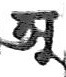
\includegraphics[height=8.0mm]{a.jpg} a  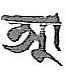
\includegraphics[height=8.0mm]{aa.jpg} ā 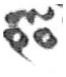
\includegraphics[height=8.0mm]{i.jpg} i 
\includegraphics[height=8.0mm]{ii.jpg} ī

\includegraphics[height=8.0mm]{u.jpg} u  
\includegraphics[height=8.0mm]{uu.jpg} ū 
\includegraphics[height=8.0mm]{white.jpg} ṛ 
\includegraphics[height=8.0mm]{white.jpg} ṝ \\

\includegraphics[height=8.0mm]{white.jpg} ḷ 
\includegraphics[height=8.0mm]{white.jpg} ḹ 
\includegraphics[height=8.0mm]{e.jpg} e 
\includegraphics[height=8.0mm]{white.jpg} ai \\
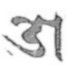
\includegraphics[height=8.0mm]{o.jpg} o 
\includegraphics[height=8.0mm]{white.jpg} au 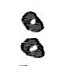
\includegraphics[height=8.0mm]{anu1.jpg} ḥ 
\includegraphics[height=8.0mm]{anu2.jpg} ḥ \\
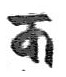
\includegraphics[height=8.0mm]{ka.jpg} ka 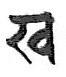
\includegraphics[height=8.0mm]{kha.jpg} kha 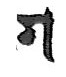
\includegraphics[height=8.0mm]{ga.jpg} ga 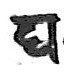
\includegraphics[height=8.0mm]{gha.jpg} gha
\includegraphics[height=8.0mm]{white.jpg} ṅa\\
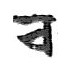
\includegraphics[height=8.0mm]{ca.jpg} ca 
\includegraphics[height=8.0mm]{white.jpg} cha 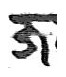
\includegraphics[height=8.0mm]{ja.jpg} ja 
\includegraphics[height=8.0mm]{white.jpg} jha 
\includegraphics[height=8.0mm]{white.jpg} ña\\

\includegraphics[height=8.0mm]{white.jpg} ṭa 
\includegraphics[height=8.0mm]{white.jpg} ṭha 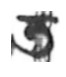
\includegraphics[height=8.0mm]{rda.jpg} ḍa  
\includegraphics[height=8.0mm]{white.jpg} ḍha 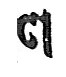
\includegraphics[height=8.0mm]{rna.jpg} ṇa\\
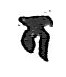
\includegraphics[height=8.0mm]{ta.jpg} ta 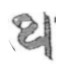
\includegraphics[height=8.0mm]{tha.jpg} tha 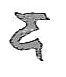
\includegraphics[height=8.0mm]{da.jpg} da 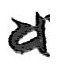
\includegraphics[height=8.0mm]{dha.jpg} dha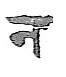
\includegraphics[height=8.0mm]{na.jpg} na \\
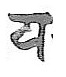
\includegraphics[height=8.0mm]{pa.jpg} pa 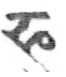
\includegraphics[height=8.0mm]{pha.jpg} pha 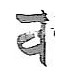
\includegraphics[height=8.0mm]{ba.jpg} ba 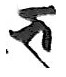
\includegraphics[height=8.0mm]{bha.jpg} bha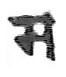
\includegraphics[height=8.0mm]{ma.jpg} ma \\
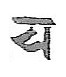
\includegraphics[height=8.0mm]{ya.jpg} ya 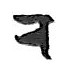
\includegraphics[height=8.0mm]{ra.jpg} ra 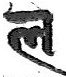
\includegraphics[height=8.0mm]{la.jpg} la 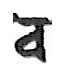
\includegraphics[height=8.0mm]{va.jpg} va \\
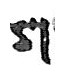
\includegraphics[height=8.0mm]{sha.jpg} śa 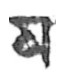
\includegraphics[height=8.0mm]{ssa.jpg} ṣa 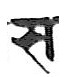
\includegraphics[height=8.0mm]{sa.jpg} sa \\
\includegraphics[height=8.0mm]{ha.jpg} ha \\
 
\subsubsection{Konsonanten mit Vokalen}

Da für keinen Konsonanten alle Kombinationen mit allen Vokalen vorhanden sind, greife ich auf Beispiele mehrerer Konsonanten zurück, beginnend mit ka. Abgesehen von der Kombination aus Konsonant und Vokal e, bei dem es zwei Schreibweisen gibt, folgen alle Konsonanten in Kombination mit den Vokalen dem hier abgebildeten Schema. Konsonantenkombinationen mit ṛ ṝ ḷ und ḹ sind im Manuskript nicht vorhanden. \hfill \break  
\linebreak
\\
\noindent
\includegraphics[height=8.0mm]{ka.jpg} ka \includegraphics[height=8.0mm]{kaa.jpg} kā \includegraphics[height=8.0mm]{khi.jpg} khi \includegraphics[height=8.0mm]{kii.jpg} kī \includegraphics[height=8.0mm]{ku.jpg} ku \includegraphics[height=8.0mm]{puu.jpg} pū \includegraphics[height=8.0mm]{kr.jpg} kṛ \includegraphics[height=8.0mm]{white.jpg} kṝ \includegraphics[height=8.0mm]{white.jpg} kḷ \includegraphics[height=8.0mm]{white.jpg} kḹ \includegraphics[height=8.0mm]{ge.jpg} ge \includegraphics[height=8.0mm]{te.jpg} te\footnote{Man beachte die beiden Schreibweisen für Konsonant mit e.} \\ \includegraphics[height=8.0mm]{yai.jpg} yai \includegraphics[height=8.0mm]{ko.jpg} ko \includegraphics[height=8.0mm]{kau.jpg} kau \includegraphics[height=8.0mm]{kam.jpg} kaṃ \includegraphics[height=8.0mm]{kam2.jpg} kaṃ \includegraphics[height=8.0mm]{kah.jpg} kaḥ 

\subsubsection{Verschiedene Ligaturen}

Die folgende Liste beinhaltet neben den wichtigsten auch alle weniger offensichtlichen und schwierigeren Ligaturen. \hfill \break
\linebreak
\\
\includegraphics[height=8.0mm]{kt.jpg} kti \includegraphics[height=8.0mm]{krā.jpg} krā \includegraphics[height=8.0mm]{kre.jpg} kre \includegraphics[height=8.0mm]{kva.jpg} kva \includegraphics[height=8.0mm]{kssa.jpg} kṣa  \includegraphics[height=8.0mm]{kṣī.jpg} kṣī \includegraphics[height=8.0mm]{kyam.jpg} khyaṃ \includegraphics[height=8.0mm]{gra.jpg} gra \includegraphics[height=8.0mm]{nge.jpg} ṅge \includegraphics[height=8.0mm]{ngu.jpg} ṅgu\\
\noindent
\includegraphics[height=8.0mm]{ccha.jpg} ccha \includegraphics[height=8.0mm]{cchū.jpg} cchū \includegraphics[height=8.0mm]{cya.jpg} cya \includegraphics[height=8.0mm]{jna.jpg} jña \includegraphics[height=8.0mm]{jne.jpg} jñe \includegraphics[height=8.0mm]{jyo.jpg} jyo \includegraphics[height=8.0mm]{nge.jpg} ñge \includegraphics[height=8.0mm]{nca.jpg} ñca \includegraphics[height=8.0mm]{nci.jpg} ñci \includegraphics[height=8.0mm]{nja.jpg} ñja \\
\noindent
\includegraphics[height=8.0mm]{rtc.jpg} ṭca \includegraphics[height=8.0mm]{ttam.jpg} ṭṭaṃ \includegraphics[height=8.0mm]{rtbi.jpg} ṭbi \includegraphics[height=8.0mm]{rdd.jpg} ḍḍi \includegraphics[height=8.0mm]{rnde.jpg} ṇḍe \includegraphics[height=8.0mm]{ntha.jpg} ṇṭha \includegraphics[height=8.0mm]{nnda.jpg} ṇḍa \includegraphics[height=8.0mm]{nny.jpg} ṇya \\
\noindent
\includegraphics[height=8.0mm]{tkaa.jpg} tkā \includegraphics[height=8.0mm]{tta.jpg} tta \includegraphics[height=8.0mm]{tni.jpg} tni \includegraphics[height=8.0mm]{tmuu.jpg} tmū \includegraphics[height=8.0mm]{trai.jpg} trai \includegraphics[height=8.0mm]{tvaa.jpg} tvā \includegraphics[height=8.0mm]{dghaa.jpg} dghā \includegraphics[height=8.0mm]{dca.jpg} dca \includegraphics[height=8.0mm]{dda.jpg} dda \includegraphics[height=8.0mm]{ddhru.jpg} ddhru \includegraphics[height=8.0mm]{ddhyaa.jpg} ddhyā \includegraphics[height=8.0mm]{ddhr.jpg} ddhṛ \includegraphics[height=8.0mm]{dhye.jpg} dhye \includegraphics[height=8.0mm]{dya.jpg} dya \includegraphics[height=8.0mm]{dram.jpg} draṃ \includegraphics[height=8.0mm]{dvir.jpg} dvir \includegraphics[height=8.0mm]{dhya.jpg} dhya \includegraphics[height=8.0mm]{nta.jpg} nta \includegraphics[height=8.0mm]{nthim.jpg} nthiṃ \includegraphics[height=8.0mm]{nda.jpg} nda \includegraphics[height=8.0mm]{ndro.jpg} ndro \includegraphics[height=8.0mm]{nna.jpg} nna \\
\noindent
\includegraphics[height=8.0mm]{pra.jpg} pra \includegraphics[height=8.0mm]{bdhvaa.jpg} bdhvā \includegraphics[height=8.0mm]{bru.jpg} bru \includegraphics[height=8.0mm]{bhyaa.jpg} bhyā \includegraphics[height=8.0mm]{mṇā.jpg} mṇā \includegraphics[height=8.0mm]{mya.jpg} mya \\ 
\noindent
  \includegraphics[height=8.0mm]{rgga.jpg} rgga \includegraphics[height=8.0mm]{rṇṇa.jpg} rṇṇa \includegraphics[height=8.0mm]{rddhvaṃ.jpg} rddhvaṃ \includegraphics[height=8.0mm]{lla.jpg} lla \includegraphics[height=8.0mm]{vyu.jpg} vyu \\ 
\noindent
\includegraphics[height=8.0mm]{śca.jpg} śca \includegraphics[height=8.0mm]{ṣṭha.jpg} ṣṭha \includegraphics[height=8.0mm]{spha.jpg} spha \includegraphics[height=8.0mm]{smṛ.jpg} smṛ \\
\noindent
\includegraphics[height=8.0mm]{hneḥ.jpg} hneḥ \includegraphics[height=8.0mm]{hmā.jpg} hmā \includegraphics[height=8.0mm]{hya.jpg} hya

\clearpage

\subsubsection{Zeichen}
\includegraphics[height=8.0mm]{siddham.jpg} \textit{siddham} \includegraphics[height=8.0mm]{daṇḍa.jpg} \textit{daṇḍa} \includegraphics[height=8.0mm]{doubledaṇḍa.jpg} Doppel-\textit{daṇḍa} \includegraphics[height=8.0mm]{viramat.jpg} \textit{virāma} nach ta \includegraphics[height=8.0mm]{avagraha.jpg} \textit{avagraha}
\\
\includegraphics[height=8.0mm]{visarga1.jpg} \textit{visarga} \includegraphics[height=8.0mm]{visarga2.jpg} \textit{visarga} \includegraphics[height=4.0mm]{zeichenx.png} \textit{visarga}?\footnote{Man beachte die unterschiedlichen Schreibweisen des \textit{visarga}.}
\\ \\\includegraphics[height=4.0mm]{anusvara.jpg} \textit{anusvāra} \includegraphics[height=4.0mm]{anusvara1.jpg} \textit{anusvāra} \includegraphics[height=4.0mm]{anusvara2.jpg} \textit{anusvāra} \\ \\
\includegraphics[height=2.0mm]{nevarikomma.jpg} \textit{Nevārī-Komma} \\ \\
\includegraphics[height=8.0mm]{luecke.jpg} \textit{Lückenfüller-Symbol}


\subsubsection{Zahlen 1-10}
Ich beschränke mich hier auf die Abbildung der Zahlen 1-10. Alle weiteren im Manuskript vorkommenden Zahlen bis 65 werden aus den 10 Grundzahlen zusammengesetzt.\footnote{Man beachte die beiden Varianten der Zahl 6.}
\linebreak
\\ 
\includegraphics[height=8.0mm]{z1.jpg} 1 \includegraphics[height=8.0mm]{z2.jpg} 2 \includegraphics[height=8.0mm]{z3.jpg} 3 \includegraphics[height=8.0mm]{z4.jpg} 4 \includegraphics[height=8.0mm]{z5.jpg} 5 \includegraphics[height=8.0mm]{z6.jpg} 6 \includegraphics[height=8.0mm]{z6x.jpg} 6 \includegraphics[height=8.0mm]{z7.jpg} 7 \includegraphics[height=8.0mm]{z8.jpg} 8 \includegraphics[height=8.0mm]{z9.jpg} 9 \includegraphics[height=8.0mm]{z10.jpg} 10
\clearpage
\subsection{Das Metrum}

Das GYŚ ist vollstänig im \textit{anuṣṭubh}-Metrum kompiliert. Die epische \textit{anuṣṭubh} ist ein zweizeiliger Vers. Jeder Vers beinhaltet 32 Silben, die in vier Viertelverse eingeteilt sind. Somit besteht jeder \textit{pāda} aus 8 Silben. Ein einzeiliges Hemistichion enthält also zwei \textit{pāda}s mit 2 x 8 Silben und ein ganzer \textit{anuṣṭubh}-Vers vier \textit{pāda}s mit 4 x 8 Silben. Jedes Hemistichion mit 16 Silben kann entweder eine \textit{pathyā}-Form (``normale''-Form), oder verschiedene \textit{vipulā}-Formen annehmen.

\textbf{Normale und Allgemeine Form des GYŚ Vers:}
\begin{itemize}
 \item{1, 3, 4, 5, 6, 7, 8, 9, 10, 11, 12, 13, 14, 15, 16, 17, 18, 19, 20, 21, 22, 23, 24, 25, 26, 27, 28, 29, 30, 31, 32, 33, 34, 35, 36, 37, 39, 40, 42, 43, 44, 45, 46, 47, 48, 49, 50, 52, 53, 54, 55, 56, 57, 58, 59, 61, 62, 63, 64, 65}
  \end{itemize}

\textbf{Metrische Fehler der originalen Handschrift:}
\begin{itemize}
\item{2\textsuperscript{d} (fünfte Silbe ``śrī'' ist lang, sollte aber kurz sein)}
\item{41\textsuperscript{c-d} (ist \textit{hemarūpam})}
\item{51 (eine Silbe fehlt, Manuskript weist in diesem Vers starke Beschädigung auf)}
\end{itemize}

\textbf{Sonderformen (\textit{vipulā})}:
\begin{itemize}
\item{38}
\end{itemize}

%WoW Nils denk hier bitte an das schöne leichte Kapitel im Lehmann über Anustubh.Dann nochmal alles durchcounten.

\subsection{Datierung}
\label{datierung}

Eine Datierung des GYŚ-\textit{codex unicus}, dessen Kompilationsdatum auf keinem der verfügbaren Folios schriftlich fixiert wurde, kann zunächst anhand paläographischer Beobachtungen zeitlich eingegrenzt werden. Vor allem durch die historische Verortung der verwendeten Schrift, nämlich \textit{Nepālākṣara}, das mit Abstand gebräuchlichste Alphabet, um Sanskrit und klassisches Nevārī in Nepal mindestens ab dem 11. Jh. zu schreiben. \textit{Nepālākṣara} existierte dort parallel zu \textit{Devanāgarī}, welches bereits seit 1019 n. u. Z. in Inschriften des Kathmandu Tals zu finden ist und anderen Schriftvarianten wie \textit{Golamola} (der ``ballköpfige'' Typus), \textit{Bhu(ṃ)ji(ṃ)ola} (der ``fliegenköpfige'' Typus), \textit{Kūṃmola} (der ``punktköpfige'' Typus) und \textit{Pācumola} (der ``ebenköpfige'' Typus). Die in dieser Region und Zeit uns erhaltenen buddhistischen Texte wurden meist in der reichlich verzierten \textit{Rañjanā}-Schrift geschrieben, und die älteste Gruppe der \textit{Nevārī}-Manuskripte in \textit{Bhujiṃmola}. Beide Schriften wurden jedoch bis zum Ende der Malla Periode\footnote{Die frühe Malla-Periode beginnt 1200 n. u. Z.  bis 1482 n. u. Z. und erstreckt sich über die Herrschaft von König Arimalla (1200-1216 n. u. Z.) und König Jayayakṣa Malla (1428-1482). Die Periode der darauffolgenden drei Malla Königreiche von 1492 bis 1768 n. u. Z. \parencite[xi]{lienhard1988}.} im Jahr 1768 n. u. Z. benutzt, aber zunehmend von \textit{Nepalākṣara} abgelöst \parencite[xviii]{lienhard1988}.
Anhand einer klar erkennbaren Entwicklung vom Gebrauch bestimmter Zeichen, die beispielsweise in den Tabellen von \parencite{bendall1992} zusammen mit einer Datierung aufgelistet sind und einem morphologischen Entwicklungsprozess unterliegen, sowie weiteren Vergleichen mit eindeutig datierten Manuskripten\footnote{\raggedright{Hierfür wurden primär die digitalisierten und katalogisierten \textit{Nepalākṣara}-Sanskrit-Manuskripte der Cambridge Digital Library verwendet. Siehe https://cudl.lib.cam.ac.uk/collections/sanskrit (14.05.2018).}} aus Nepal, kann der mögliche Kompilationszeitraum des Manuskriptes präziser eingegrenzt werden.

\begin{figure}[ht]
	\centering
  \includegraphics[width=1\textwidth, height=350pt]{bendall1.jpg}
	\caption{Buchstabentabelle nach \parencite[233]{bendall1992}.}
	\label{fig1}
\end{figure}
 
Das im GYŚ-\textit{codex unicus} vorkommende Zeichen für e \includegraphics[height=4.0mm]{paleo_e.png} entspricht dem bei \parencite[233]{bendall1992} vermerkten e, welches auf das Jahr 1385 n. u. Z. in MS. Add 1395 datiert wurde\footnote{\raggedright{Für eine detaillierte Beschreibung von \textcite{pancaraksa}, MS Add. 1395 siehe https://cudl.lib.cam.ac.uk/view/MS-ADD-01395/1 (14.05.2018).}} und sich bis 1450 n. u. Z. nur minimal verändert. Dieser Verwendung geht, wie in \parencite[233]{bendall1992} gezeigt wird, bis ca. 1139 n. u. Z. die ältere Form des geschlossenen e voraus. Ähnliches ist beim Buchstaben tha \includegraphics[height=4.0mm]{paleo_th.png} zu beobachten. Ab ca. 1576 n. u. Z. wird das e, wie in der Tabelle zu sehen ist, mit einem ausgeprägteren Haken im oberen Abschnitt des \textit{akṣara}s geschrieben. Allerdings entsprechen die anderen der morphischen Veränderung unterworfenen \textit{akṣara}s des \textit{Nepalākṣara}-Alphabetes in MS. Add. 1395, abgesehen von ta \includegraphics[height=4.0mm]{paleo_ta.png}, dha \includegraphics[height=4.0mm]{paleo_dh.png} und śa \includegraphics[height=4.0mm]{paleo_sh.png}, nicht denen des GYŚ, sondern sind in der \textit{Bhujiṃmola}-Variante abgefasst. Abgesehen von dem eben vermerkten Buchstaben e, nebst dha, tha und minimal nuanciertem pha und bha, entsprechen alle bei \parencite[233]{bendall1992} vermerkten weiteren Buchstaben, nämlich kha \includegraphics[height=4.0mm]{paleo_kh.png}, ja \includegraphics[height=4.0mm]{paleo_ja.png}, ṇa \includegraphics[height=4.0mm]{paleo_nna.png}, la \includegraphics[height=4.0mm]{paleo_la.png}, śa \includegraphics[height=4.0mm]{paleo_sh.png} und ṣa \includegraphics[height=4.0mm]{paleo_ssa.png}, exakt denen des auf 1139 n. u. Z. datierten \textit{Śivadharma-corpus}\footnote{\raggedright{Für eine detaillierte Beschreibung des \textcite{sivadharma}, MS Add. 1645 inkl. Faksimilie siehe https://cudl.lib.cam.ac.uk/view/MS-ADD-01645/1 (14.05.2018).}}. Insbesondere der Buchstabe pha des \textit{Śivadharma corpus}, der sich in dieser Schreibweise im Manuskript des GYŚ befindet, taucht nach Bendalls Tabelle nur noch bis ca. 1450 n. u. Z. in den \textit{Nepalākṣara}-Manuskripten auf. Das dha \includegraphics[height=4.0mm]{paleo_dh.png} des GYŚ kann ebenfalls in MS Add. 1409, dem \textit{Rāmāṅkanāṭikā}\footnote{\raggedright{Für eine detaillierte Beschreibung von \textcite{ramakantika}, MS Add. 1409 inkl. Faksimile siehe https://cudl.lib.cam.ac.uk/view/MS-ADD-01409-00001/5 (14.05.2018).}}, welches auf das Jahr 1360 n. u. Z. datiert wird, nachgewiesen werden, welches im 15. Jh. n. u. Z. in dieser Form durch neue Varianten abgelöst wird \parencite[233]{bendall1992}. Es lässt sich demnach, anhand der hier zur Verwendung kommenden Materialien, relativ sicher einschätzen, dass der vorliegende \textit{codex unicus} des GYŚ \textit{akṣaras} aufweist, welche zwischen den Jahren 1139 und 1450 n. u. Z. und darüber hinaus bis maximal Ende des 15. Jh. in Gebrauch waren, danach nicht mehr. 

Ein weiterer wichtiger paläographischer Aspekt, der bei der Datierung des GYŚ-Kodex wichtige Anhaltspunkte liefert, ist die Verwendung von Zahlsymbolen.

\begin{figure}[ht]
	\centering
  \includegraphics[width=1\textwidth, height=350pt]{bendall3.jpg}
	\caption{Zahlensymbole nach \parencite[liv]{bendall1992}.}
	\label{fig2}
\end{figure}
 
Vor allem sind, wie hier zu sehen ist, die Zahlen 4, 5, und 6 der morphologischen Veränderung unterworfen \parencite[liv]{bendall1992}. Werden die Ziffern des GYŚ-Manuskriptes 4 \includegraphics[height=4.0mm]{paleo_4.png}, 5 \includegraphics[height=4.0mm]{paleo_5.png} und 6 \includegraphics[height=4.0mm]{paleo_6.png} mit denen verglichen, die Bendall in seiner Tabelle \parencite[235]{bendall1992} auflistet, kann festgestellt werden, dass die 4 von MS Add. 1644\footnote{\raggedright{Für eine detaillierte Beschreibung von \textcite{pancaraksa2}, MS Add. 1644 inkl. Faksimile siehe https://cudl.lib.cam.ac.uk/view/MS-ADD-01644/4 (14.05.2018).}}, der der \textit{Pañcarakṣā} entspricht, welches auf das Jahr 1205 n. u. Z. datiert wird. Allerdings weicht vor allem die Verwendung der Zahl 6 deutlich von der hiesigen 6 ab, wohingegen die 5 sehr ähnlich ist. Die Zahlen 5 und 6 unseres Manuskriptes entsprechen genau denen von MS Add. 1708\footnote{Für MS Add. 1708 ist kein Eintrag in der Cambridge Digital Library vorhanden. Siehe anstattdessen \parencite[203]{bendall1992}.}, welches von Bendall zwischen dem 15. und 16. Jh. n. u. Z. datiert wird. Hier weichen jedoch die Zahlsymbole für 1-3 merklich ab. Diese entsprechen wiederum nahezu exakt den Zahlensymbolen für 1-3 von MS. Add. 1395, MS. Add. 1683\footnote{\raggedright{Für eine detaillierte Beschreibung von MS. Add. 1683 (\textit{Saddharmapuṇḍarīka}) aus dem Jahr 1093 n. u. Z. siehe https://cudl.lib.cam.ac.uk/view/MS-ADD-01683/1 (14.05.2018).}} und MS Add. 1684\footnote{\raggedright{Für eine detaillierte Beschreibung von \textcite{saddharma}, MS. Add. 1684 inkl. Faksimile siehe https://cudl.lib.cam.ac.uk/view/MS-ADD-01684-00001/1 (14.05.2018).}}, wobei hier wiederum die Ziffern 4, 5 und 8 deutlich von denen des hiesigen Ms abweichen.

Werden diese hier aufgeführten Aspekte nun mit einem weiteren Feld von paelographischen Kriterien verglichen, wie beispielsweise die Größe, Struktur, Bindelochplatzierung, die Art der Nummerierung mit bereits datierten Manuskripten, dann können wir den höchsten Grad der Ähnlichkeit mit MS Add. 1685\footnote{\raggedright{Für eine detaillierte Beschreibung von \textcite{amara}, MS Add. 1686 siehe https://cudl.lib.cam.ac.uk/view/MS-ADD-01685/4 (14.05.2018).}}(\textit{``Amarakośa''}, datiert auf das Jahr 1380 n. u. Z. und dem MS Add. 1580\footnote{\raggedright{Für eine detaillierte Beschreibung von \textcite{shambuvadana}, MS Add. 1580 siehe https://cudl.lib.cam.ac.uk/view/MS-ADD-01580/10 (14.05.2018).}} (\textit{``Śambūkāvadāna''}), welches auf 1427 n. u. Z. datiert werden kann, feststellen. Beide weisen den von allen in der Cambridge University Library gelisteten Handschriften in \textit{Nepalākṣara} höchsten Ähnlichkeitsgrad hinsichtlich der betrachteten paläographischen Kritierien auf. Die kumulative Evidenz der untersuchten Kriterien lässt die Niederschrift des hier zu datierenden \textit{codex unicus} zwischen 14. und 15. Jh. n. u. Z. am wahrscheinlichsten erscheinen. 

Es ist nicht auszuschließen, dass die Kompilation des Werkes hingegen bereits vorher stattfand. Der primäre Grund ist die Verbindung des GYŚ zur \textit{Amṛtasiddhi}, aus denen das GYŚ einige Verse entleiht und dessen Inhalte es paraphrasiert. Die \textit{Amṛtasiddhi} wird auf das 11. Jh. n. u. Z. datiert \parencite[2]{mallinson2016as}. Somit dürfte das GYŚ irgendwann zwischen dem 11. und 15. Jh. verfasst worden sein. Einen weiteren Hinweis, der zwar erwähnenswertist, aber eher schwache Evidenz liefert, ist ein paralleler Halbvers mit der \textit{Śārṅgadharapaddhati}\footnote{GYŚ 21\textsuperscript{c-d} entspricht Śp 255.45\textsuperscript{a-b}.}, welches 1363 n. u. Z. kompiliert wurde \parencite[18]{olesen2016}. Es ist jedoch für mich ohne Weiteres nicht abschätzbar, ob und wer diesen Vers von wem übernahm.

%\begin{itemize}
%\item \url{https://cudl.lib.cam.ac.uk/view/MS-ADD-01685/4} Amarakośa (MS Add.1685) Date of Creation: 500 Nepāla / 1380 CE. -> sehr sehr ähnlich Material, Schriftzeichen, Nummerierung

%\item \url{https://cudl.lib.cam.ac.uk/view/MS-ADD-01580/10} Śambūkāvadāna (MS Add.1580) Date of Creation: 547 Nepāla / 1427 CE. -> super ähnlich und es hat sogar die richtige 4!!!

%\item \url{https://cudl.lib.cam.ac.uk/view/MS-ADD-01645/4} Śivadharma corpus (MS Add.1645) Date of Creation: First codicological unit (kernel): 259 Nepāla / 1139 CE. -> auch sehr ähnlich und richtige 4 !!!\parencite[??]{bendall1992}
%\item \url{https://cudl.lib.cam.ac.uk/view/MS-ADD-01644/4} Pañcarakṣā (MS Add.1644) Pañcarakṣā (MS Add.1644) Date of Creation: 325 Nepāla / 1205 CE.  Bendall (1883: 152-153), 


%\item \url{https://cudl.lib.cam.ac.uk/view/MS-OR-00148/8} Subantaratnākara (MS Or.148) Date of Creation: 540 Nepāla / 1420 CE. Verified date: Wednesday, August 14th.

%\item \url{https://cudl.lib.cam.ac.uk/view/MS-ADD-01649/10} Siddhisāra (MS Add.1649) Date of Creation: 532 Nepāla Saṃvat / Sunday, November 11th, 1411 CE. aber in Bujjimol

%\item \url{https://cudl.lib.cam.ac.uk/view/MS-ADD-01479/44} Bṛhajjātakavivaraṇa (MS Add.1479) Date of Creation: 666 Nepāla / 1546 CE (the date is also given in the last of the initial blank folios as the date when the manuscript was started).

%\item \url{https://cudl.lib.cam.ac.uk/view/MS-ADD-01698/5} Nāmasaṅgītiṭippanī (MS Add.1108) 1392 CE.
%\item \url{https://cudl.lib.cam.ac.uk/view/MS-ADD-01161/7} Śiṣyalekha (MS Add.1161) 1084 A.D. 
%\item \url{https://cudl.lib.cam.ac.uk/view/MS-ADD-01409-00001/5} Rāmāṅkanāṭikā (MS Add.1409.1) Date of Creation: First codicological unit (kernel): 480 Nepāla / 1360 CE. Date of Creation: Second codicological unit: 15th-16th century.
%\item \url{https://cudl.lib.cam.ac.uk/view/MS-ADD-02137/10} Newārī work on legal matters, unidentified Newārī text, Mānavanyāyaśāstraṭīkā (MS Add.2137) Date of Creation: 527 Nepāla / 1407 CE.
%\item \url{https://cudl.lib.cam.ac.uk/view/MS-ADD-01354-00001/10} Dhanañjayanighaṇṭu (MS Add.1354.1) Date of Creation: 572 Nepāla / 1452 CE.

%\end{itemize}

\section{Editorische Methode}
\label{edmeth}

Diese Arbeit orientiert sich in ihrer editorischen Methode an rezenten Editionen von \textit{codices unici}.\footnote{Hier wären zu nennen: \textit{Jinendrabuddhiś Viśālāmalavatī Pramāṇasamuccayaṭīkā - Chapter 1 - Part 1: Critical Edition} und \textit{Part II: Diplomatic Edition} (2005) von Ernst Steinkellner, Helmut Krasser und Horst Lasic, sowie \textit{Vasubandhu's Pañcaskandaka: Critically Edited} (2008) von Li Xuezhu und Ernst Steinkellner, außerdem \textit{Adhyardhaśatikā Prajñāpāramitā - Sanskrit and Tibetan Texts: Critically edited} (2009) von Toru Tomabechi, Jowita Kramers \textit{Sthiramati's Pañcaskandhavibhāṣa - Part I: Critical Edition and Part II: Diplomatic Edition}, Liu Zhens \textit{The Dharmadhātustava: A Critical Edition of the Sanskrit text with the Tibetan and Chinese Translations, a Diplomatic Transliteration of the Manuscript and Notes} (2015) und Andrea Acris \textit{Dharma Pātañjala} (2011). Zwar behandelt die hier selektierte Literatur keine frühen Haṭhayoga-Handschriften, aber sie veranschaulicht exemplarisch rezente und funktionierende editorische Vorgehensweisen des indologisch-philologischen Arbeitsfeldes für die Bearbeitung von \textit{codices unici}. Darüber hinaus ist Andrea Acris \textit{Dharma Pātañjala} (2011), hierunter einer der wenigen Autoren, der die theoretischen Konstituenten und divergierenden Ansätze in wichtigen Ausschnitten der Disziplingeschichte des Editierens von südasiatischen und südostasiatischen \textit{codices unici} diskutiert \parencite[81-98]{acri2011dharma}.} Abgesehen von Andrea Acris Werk bieten diese Editionen die Lösung, basierend auf den diesen Arbeiten zu Grunde liegenden Materialien, trotz des Vorhandenseins nur eines einzigen Manuskriptes und einer oder mehrerer Übersetzungen in chinesischer oder tibetischer Sprache, sowie parallelen Passagen aus verwandten Werken, neben einer diplomatischen Edition ebenfalls eine kritische Edition anzufertigen. Andrea Acri (2011) verlässt sich bei seiner Arbeit mit dem ihm vorliegenden alt-javanesischen \textit{codex unicus} hingegen fast ausschließlich auf seine interpretativen Bemühungen, geleitet von der internen Evidenz, die im gesamten Text gefunden wird und wenn möglich durch parallele Passagen in eng verwandter Literatur, die ggf. dabei hilft, den Inhalt und Kontext eines bestimmten Textabschnittes zu rekonstruieren bzw. zu reinigen \parencite[89]{acri2011dharma}. Trotz des spärlichen Materials verschreibt sich Acri in seiner Edition der Ansicht von Goodall (1998): \begin{quote} ``An editor's not challenging bad manuscript readings can do more damage to the text than offering unsatisfactory conjectures.`` \parencite[cxiv]{goodall1998}\end{quote} Wird von den chinesischen und tibetischen Übersetzungen der jeweiligen Texte von Steinkellner etc. abgesehen und davon ausgegangen, dass die Autoren solcher historischer Übersetzungen nicht selten nur ein Manuskript vorliegen hatten (welches ggf. weniger verderbt war als das heute uns vorliegende Sanskrit-Original, oder auch nicht) und ihre Übersetzungen wiederum wahrscheinlich auf der \textit{divinatio} eben dieser Übersetzer beruht, so weisen die Editionen von Steinkellner etc. ganz ähnliche Vorraussetzungen auf, wie sie bei Acri vorhanden sind. Dieser äußert sich diesbezüglich: \begin{quote} ``The fact that the evidence documenting a manuscript happens to have been preserved only in one copy does not necessarily justify, I believe, the limitations that editors dealing with \textit{codices unici} have often imposed upon themselves. Indeed it may be argued that critical editions of \textit{codices unici} and of texts documented through several manuscripts differ only with regard to the amount of evidence and of the inferential process leading from evidence to the constituted text.'' \parencite[89]{acri2011dharma} \end{quote}   

Weil diese Situation auch für das GYŚ vorliegt, können und sollten philologisch-kritische Verfahren mit dem derzeit verfügbaren Material zur Rekonstitution einer verständlichen und übersetzbaren Ausgabe des GYŚ angewandt werden, unter Vorbehalt der Möglichkeit, dass durch zukünftiges Material eine bessere hermeneutische Annährung an den ``Text des Werkes'' des GYŚ möglich sein könnte. Jeder Editor unterliegt der Subjektivität seiner individuellen Ausbildung, seines Talents, Eifers und dem individuellen Möglichkeitsspektrum der Zuhilfenahme von Meinungen anderer Gelehrter, welche ähnlichen Parametern der Subjektivität unterliegen. Dies kann zu unterschiedlichen Ergebnissen und Meinungen führen, gerade bei begrenzter Quellenlage. Hier sollte nun betont werden, dass es in dieser Edition somit durchaus im Bereich des Möglichen liegt, dass manche am Text vorgenommenen Veränderungen in der ursprünglichen Kompilation nicht vorhanden waren und somit ein Text konstituiert wird, den es historisch in dieser Form niemals gegeben hat. Durch die parallele Anfertigung einer diplomatischen Edition wird jedoch durch die praktische Trennung der beiden theoretischen Kategorien, dem ``Text des Dokumentes'' und dem ``Text des Werkes''\footnote{Siehe hierzu \parencite[insbes. Kapitel 1]{tanselle1989}.} diesem Umstand adäquat Rechnung getragen und Konfusion vermieden, sodass der kritische Leser sich problemlos seine eigene Meinung bilden kann und sollte. Die sich hieran anknüpfende editorische Methode ergibt sich aus den verfügbaren Materialen zur kritischen Rekonstitution des Textes. Das editorische Vorgehen wird in den folgenden Abschnitten näher erläutert: \\

Für die Konstitution eines ``Text des Werkes'' des GYŚ, liegen neben dem \textit{codex unicus} eine nicht unbedeutende Menge an parallelen Versen aus der \textit{Amṛtasiddhi}, \textit{Prāṇatoṣinī} und anderen Texten\footnote{Siehe eine Liste der Zeugen, aus denen das GYŚ zitiert, von denen Verse mit GYŚ geteilt werden und derer, die Verse aus dem GYŚ zitieren oder eng verwandte Inhalte teilen, auf S.\pageref{zeugsigla}.} vor, mit deren Hilfe es möglich ist, zahlreiche Emendationen der problematischen Passagen des Texten vorzunehmen. Andere Fehler des Textes sind selbsterklärend, kosmetisch oder trivialer Natur. Wenn die Verbesserung sich nicht durch parallele Passagen anderer Texte abdecken lässt oder nicht selbsterklärend sind, werden diese als Konjektur, als spekulative Annahme im kritischen Apparatus mit der Abkürzung ``conj.'' gekennzeichnet. Die entsprechende Stelle wird in diesem Fall in der Übersetzung jedes Mal mit einer Fußnote versehen, in welcher die Gründe des vorgenommenen Eingriffs am Text erläutert werden. Wie Andrea Acri \parencite[81]{acri2011dharma} anmerkt, repräsentieren die nun bereits mehrmals genannten Kategorien ``Text des Dokumentes'' und ``Text des Werkes'' zwei unterschiedliche Aspekte des vorliegenden Textes und des Umgangs mit diesem. Der Text beinhaltet eine immaterielle, 'mentale' Komponente und eine materielle, d.h. der Text als physisches Objekt. Eine Vermischung beider Kategorien würde problematische Konsequenzen nach sich ziehen, denn ein in einer kritischen Edition rekonstruierter ``Text des Werkes'' führt zum Verlust eines Teils der historischen Evidenz \parencite[29]{tanselle1989}. 

Die diplomatische Edition zielt darauf ab, eine genaue Reproduktion des Textes zu erstellen, so wie sie die materielle Evidenz wiedergibt. Sie soll genau dokumentieren, wie genau diese Sanskrit Handschrift in \textit{Nepālākṣarā} aus dem 14. - 15. Jahrhundert n. u. Z. aussieht. Die kritische Edition ist vor allem darauf ausgerichtet, einen kohärenten Text zu rekonstruieren, der sich möglichst genau dem anzunähren versucht, was der Autor ausdrücken wollte, um beispielsweise die Relation zu anderen verwandten Texten des Haṭhayoga zu untersuchen\footnote{Siehe hierzu \parencite[76-77]{dehaan1973} und \parencite[17-21]{robson1988}.} oder schlichtweg eine lesbare und sinnvolle Übersetzung des historischen Dokumentes zu ermöglichen. Das Vorhandensein nur eines einzigen Manuskriptes bedingt demnach die Anfertigung einer diplomatischen Edition. Hinsichtlich des Editierens von Sanskrit und tibetischen \textit{codices unici}, merkt Hahn Folgendes an:

\begin{quote}  
``The general procedure of dealing with old and important \textit{codices unici} is that which has been applied by many responsible editors in the past: it ideally consists of the facsimile reproduction of the \textit{codex unicus} accompanied by a so-called "diplomatic" transcript of the text which represents the text "as it is", with no changes, and corrections, meticulously recording all its peculiarities like insertions, deletions, glosses, gaps (lacunae), haplographies (also known as lipography, is a scribal or typographical error where a letter or group of letters that should be written twice is written once.), dittographies (is the accidental, erroneous act of repeating a letter, word, phrase or combination of letters by a scribe or copyist) etc. Only this enables the future critical reader to form his own, independent opinion and perhaps see something which the first editor of the work failed to see.'' \parencite[52]{hahn2001} 
\end{quote}

Acri (2011) kommentiert diesbezüglich, dass Kritiker natürlich den Einwand aufbringen könnten, ob ein grundsätzlicher Nutzen solch eines unsynthetischen und platzraubenden Arrangements besteht, angesichts der Möglichkeit beide Editionen in eine zusammenzufügen, ohne einen Verlust an Information zu erleiden. Darüber hinaus könne gefragt werden, wie viele Leser das Interesse aufbringen und dazu fähig sind eine diplomatische Edition zu konsultieren \parencite[82]{acri2011dharma}. Grundsätzlich zielt laut Acri die Philologie darauf ab, Texte der Vergangenheit zugänglich zu machen. Sie trägt dabei zwei voneinander zu unterscheidende Grundgedanken mit sich, nämlich den historischen und den inhaltlichen. Einerseits sollte sowohl eine möglichst genaue Übertragung der Konzepte, welche durch die Textzeugen übermittelt werden, stattfinden, und zum anderen sollte aus historischer Sicht eine Dokumentation der Formen, in denen die Texte geschrieben worden sind, präzise durchgeführt werden. Letzteres kann wertvolle Informationen über den soziokulturellen Hintergrund und die ästhetischen Werte einer Zivilisation und ihrer Manuskriptkultur konservieren \parencite[82]{acri2011dharma}. Beide Arten der Edition behandeln unterschiedliche Probleme und liefern unterschiedliche Ergebnisse, die es aus der hier dargestellten theoretischen Perspektive zu vermeiden gilt, denn ein Konglomerat beider, würde zu einem nicht nutzerfreundlichen Hybridprodukt führen \parencite[81]{acri2011dharma}.

\subsection{Anmerkungen zur diplomatischen Edition}

Das in dieser Arbeit zur Verwendung kommende Layout der diplomatischen Transliteration, ist so angelegt, dass die Vorlage und ihr Charakter so präzise wie möglich reproduziert werden können. Daher wird die ursprüngliche Einteilung der Palmblätter, die Anzahl der Zeilen, die Lücken rund um das Bindeloch, die originale Ziffern-Nummerierung der Palmblätter, wie im Manuskript wiedergegeben. Die Nummerierung in der diplomatischen Transliteration wird originalgetreu in der Mitte des rechten Außenrands neben dem Text der \textit{verso}-Seite der Folios in eckigen Klammern ``[]'' angegeben. Auf eine Reproduktion der Buchstaben-Ziffern, die sich ebenfalls mittig am linken Außenrand der \textit{verso}-Seite befinden, wird verzichtet, da sie der Ziffern-Nummerierung der Palmblätter genau entspricht\footnote{Die Buchstabennummerierung kann den Faksimile entnommen werden.}. Zusätzlich wird jede Zeile zur Verbesserung der Übersichtlichkeit fettgegruckt und nach dem Schema ``\textbf{Folionummer}'' gefolgt von ``\textbf{Zeilennummer}'' durchnummeriert. Beispielsweise verweist ``\textbf{7a3}'' auf Folio 7a, Zeile 3. Die Randnotizen am rechten Rand von Folio 1a und unterhalb von Folio 9b wurden nicht in die diplomatische Transliteration aufgenommen und können, anhand der Faksimile, studiert werden. Alle orthographischen Varianten und Schreibfehler werden in der Transliteration so exakt wie möglich reproduziert. 

Eine zentrale editorische Entscheidung war es, entgegen beispielsweise \parencite{acri2011dharma}, die \textit{scriptio continua} nicht abzubilden, obwohl es möglich wäre zu argumentieren, dass die Teilung der \textit{scriptio continua} in einzelne Worte bereits einen dem Grundgedanken der diplomatischen Edition widersprechenden, invasiven, kritischen Eingriff darstellt. Zweifelsohne involviert dieser Eingriff die Interpretation und das Urteil des Editors auf der Basis seiner Kenntnis der Sprache, in welcher der Text geschrieben wurde, sowie die Anwendung bestimmter Konventionen. Da Acris (2011) diesbezügliche Argumente zwar überzeugen, aber sie sich auf seine spezifisch editorische Praxis eines  alt-javanesischen Textes beziehen, folge ich den Konventionen von rezenten diplomatischen Editionen von Sanskrit-Texten, wie Steinkellner etc. und somit einer strikten Trennung der \textit{scripta continua} entsprechend der konsistenten Anwendung der klassischen \textit{sandhi}-Regeln\footnote{Siehe \parencite[8-13]{stenzler}.}.   

Wie bereits in der Einleitung erwähnt, weisen die Folios 6b, 7a, 7b, 8b und 9a stark verblasste Zeilen auf, sodass Teile davon nicht mehr mit Sicherheit, oder gar nicht mehr, gelesen werden können. Mithilfe bestimmter Filter und experimenteller Veränderung der in den vorliegenden Digitalisaten vorhandenen Bildinformationen, so vor allem verschiedener Farbkanäle mit dem Bildbearbeitungsprogramm GIMP\footnote{Siehe https://www.gimp.org/ (14.05.2018) für weitere Informationen.}, konnten einige Zeichen dieser beschädigten Teile der Folios, leider nicht alle, rekonstruiert werden. An den entsprechenden Textstellen wurde jeweils am Ende der Zeile eine Fußnote eingefügt, in der eine Abbildung der zu bearbeienden Abschnitte der Digitalisate eingefügt wird, um die redaktionellen Entscheidungen nachvollziehbarer zu gestalten, und eigene Urteile fällen zu können. 

Die spezifischen Sonderzeichen im Apparatus der diplomatischen Edition werden in der Sektion ``Konventionen und Abkürzungen'' auf S.\pageref{konv} mit ihren entsprechenden Erklärungen aufgelistet.   

\subsection{Anmerkungen zur kritischen Edition}

%Die in dieser Arbeit zur Verwendung kommenden theoretischen Grundlagen und die Spezifika des kritischen Editierens von \textit{codices unici} sollen nun näher erläutert werden. In diesem Rahmen sollen für die hiesige Arbeit relevante Einblicke des aktuellen Diskurses zum Thema kritische Edition von \textit{codices unici} herausgestellt werden, um zu zeigen, warum der Begriff ``kritische Edition'' trotz der Unterschiede der kritisch-editorischen Arbeit basierend auf einem \textit{codex unicus} und der kritisch-editorischen Arbeit an einer Komposition, die auf mehreren verschiedenen Textzeugen basiert und das eine, 'beste' Manuskript zu bestimmen sucht \parencite[10-11]{molen1983}, angewendet werden sollte. Hinsichtlich dieser Diskrepanz diskutiert Acri die Ansicht von De Haan, welcher die Meinung vertritt, dass das kritische Editieren von \textit{codices unici} eine andere Methodologie benötigt als rekonstruierte kritische Editionen, die auf mehreren Textzeugen basieren \parencite[88]{acri2011dharma}. Laut De Haan versucht die kritische Edition basierend auf einem Manuskript, die verbliebene Quelle in einer so ``reinen Form wie möglich'' verfügbar zu machen - sie basiert auf einem Manuskript, hat keine Varianten, Fehler werden nur in dem Maße korrigiert wie es die Verbesserung von Schreibfehlern zulässt und Normalisierung würde nicht benötigt werden \parencite[88]{acri2011dharma}. Dem stellt Acri gegenüber, dass es unmöglich sei, die verbleibende Quelle ``in einer möglichst reinen Form'' zugänglich zu machen, indem man nur Fehler korrigiert, die im Schreibprozess entstanden sind: 

%\begin{quote} ``To me, the correction of trivial flaws of execution undermining the meaningfulness of a word, or the coherence of a series of words, in a given context may be regarded as obvious an operation as a conjectural emendation aiming at restoring the meaningfulness and logical coherence of a series of corrupted words.'' \parencite[88]{acri2011dharma} \end{quote}

In der kritischen Edition mit multiplen Textzeugen müssen die Lesarten, die der Editor versucht zu rekonstruieren auf der Basis der Evidenz der Texte, die ihm zu Verfügung stehen, vorgenommen werden. Beim kritischen Edieren von \textit{codices unici} ist der Editor, wie weiter oben erwähnt, oft auf seine interpretativen Bemühungen, bzw. seine \textit{divinatio} angewiesen. Hier stehen dem Editor neben der internen Evidenz des Textes, wenn möglich identische oder parallele Passagen von verwandter Literatur zur Verfügung, um verderbte Passagen, Fehler des Inhalts und Kontextes bestimmter Textpassagen zu rekonstruieren. Um die verderbten Passagen des GYŚ zu rekonstruieren, wurden alle zur Verfügung stehenden ``geringeren'' Zeugen\footnote{Zu den geringeren Zeugen gehören alle Texte, aus denen der Autor des GYŚ für dessen Kompilation Verse entliehen hat, sowie alle Werke, die aus dem GYŚ selbst Verse oder Passagen entliehen oder zitiert haben, und eng verwandte Literatur, deren Inhalte anderweitig zu der kritisch-editorischen Tätigkeit beitragen können. Der Begriff ``geringere Zeugen'' wurde hier gewählt, um zwischen ``direkten'' Textzeugen, nämlich dem \textit{codex unicus} und den ``indirekten'' Zeugen, nämlich den Texten, welche identische oder ähnliche Verse und Inhalte mit dem \textit{codex unicus} teilen, zu differenzieren.}, die mit dem GYŚ in Relation stehen, konsultiert. Dieser kritischen Edition des GYŚ liegen entliehene bzw. geteilte Verse des \textit{Amṛtasiddhi}, \textit{Prāṇatoṣiṇī}, \textit{Śivasaṃhita}, \textit{Śārṅgadharapaddhati}, \textit{Dhyānabindu Upaniṣad}, \textit{Varaha Upaniṣad} und \textit{Puraścaryārṇavaḥ} zu Grunde. Diese Texte decken einen nicht unbedeutenden Teil der problematischen Passagen des GYŚ ab und bieten sinnvolle alternative Lesarten an, welche den unverständlichen und verderbten Passagen einen in den meisten Fällen unzweideutigen Sinn verleihen. Die Parallelen und korrespondierenden Passagen in diesen Texten werden im ersten Register des Apparatus angeführt. Sie werden aus den genannten Gründen als geringere Textzeugen mit entsprechenden Kennzeichen klassifiziert (Siehe S.\pageref{kennz}), welche die Art der Verbindung zum GYŚ und deren Verläßlichkeitsgrad hinsichtlich der jeweiligen Passagen kennzeichnen. An dieser Stelle sei angemerkt, dass die Evidenz in den ``geringeren'' Zeugen, ab etwa der Hälfte der Verse des GYŚ immer mehr nachlässt und gegen Ende vollständig versiegt.

Darüber hinaus wurde für diese Edition die Entscheidung getroffen, entsprechend dem akademischen Standard mit der Arbeit von \textit{codices unici}, wie sie auch bei Acri, Steinkellner etc. Verwendung findet, eine Standardisierung der Rechtschreibung vorzunehmen.\footnote{Vgl. \parencite[lvi-lviii]{steinkellner2005} und \parencite[xxxiii]{kramer2013a}.} Alle Standardisierungsmaßnahmen werden unter ``Konventionen für den kritischen Text'', auf S.\pageref{konvkrit}, vermerkt.

Die kritische Edition des GYŚ beansprucht einen lesbaren Text zu präsentieren, in dem die Details des Manuskriptes, die nicht für die Wiederherstellung des ``Text des Werkes'' notwendig sind, im kritischen Apparat unberücksichtigt bleiben. Diesbezüglich wurden alle Details des Manuskriptes inkl. Faksimile vollständig in der diplomatischen Edition dokumentiert. So werden für den inhaltlichen Aspekt des ``Text des Werkes'' alle unbedeutenden Zeichen, wie \textit{Nevārī}-Kommas, Lückenfüllerzeichen, Bindelochvermerke oder \textit{virāma}s etc. von der kritischen Edition exkludiert. Korrekturen, die der Autor oder spätere Besitzer des \textit{codex} vorgenommen haben, wie die Hinzufügung oder Löschung von \textit{akṣara}s, werden ohne editorische Kennzeichnung in den Text aufgenommen. 

Jede editorische Intervention, sei es eine Emendation (em.)\footnote{Dies könnte z.B. entweder eine Korrektur von trivialen oder häufigen Fehlern sein, die beim Ab- oder Niederschreiben eines Textes entstehen, so wie ungewollte Ergänzungen oder Auslassungen von einem oder mehreren \textit{akṣara}s oder \textit{akṣara}s, \textit{anusvāra}s, rephas und anderen vokalischen Zeichen, oder mehr komplexe, aber immernoch eine relativ offensichtliche Korrektur des Textes, die durch parallele Passagen der geringeren Zeugen belegt werden kann, aber nicht muss \parencite[95]{acri2011dharma}.}, oder eine Konjektur (conj.)\footnote{Dies repräsentiert eine Intervention von eher unsicherem, jedoch nicht unwahrscheinlichem Charakter, die durch einen komplexeren Schlußfolgerungsprozess zu Stande kommt, im Gegensatz zur Emendation \parencite[95]{acri2011dharma}.}, die eine substanzielle Veränderung eines oder mehrerer Wörter betrifft und die Ebene der Orthographie überschreitet, wird im zweiten Register des Apparatus verzeichnet. Die meisten Emendationen, die im kritischen Text vorgenommen wurden, sind grammatikalischer oder orthographischer Natur. Laut Robson (1988) setzen verschiedene Genres kritisch zu editierender Texte unterschiedliche Kritieren bei der Adoption der editorischen Arbeit voraus \parencite[25]{robson1988}. Es kommt auf die Form der Überlieferung an, vor allem, ob der Text in Prosa geschrieben ist, oder als lyrischer Text einem bestimmten Versmaß folgt. Im Falle des GYŚ finden wir einen Text vor, der durchgängig im \textit{anuṣṭubh}-Metrum geschrieben wurde, sodass bei Unregelmäßigkeiten im Metrum, wie beispielsweise bei fehlenden Silben etc. eine einfachere Sanierung der betreffenden Stelle möglich wird. Im Gegensatz zu einem Prosatext, bei dem sich Editoren beispielsweise auf fixierte Muster der Satzkonstruktion und Terminologien verlassen müssen, auf welchen die interne Kohärenz der Argumente letztlich basiert \parencite[90]{acri2011dharma}. Alle Korrekturen, die sich aus einem nicht eingehaltenen Metrum ergeben, werden als \textit{metri causa} (m.c.) gekennzeichnet.    

Hinzufügungen oder Löschungen von Satzzeichen, oder einem oder mehreren Lexemen, wurden nicht im Apparatus notiert, sondern direkt in den Text inkorporiert und folgen den redaktionellen Zeichen, die auch in der diplomatischen Edition respektive Verwendung finden. Diese werden unter ``Redaktionelle Zeichen'' auf S.\pageref{redz} aufgelistet. Die beiden wichtigsten Quellen der kritisch-philologischen Entscheidungen bei allen Emendationen und Verbesserungen sind \parencite{maas1950} und \parencite{katre1954}. 

Die Zeilennummerierung folgt der Vernummerierung. Jedes Hemistichion der Verse ist aufgeteilt in zwei \textit{pāda}s zu je acht Silben. So ergeben sich je Vers zwei Zeilen mit der gleichen Nummer, die durch z.B. 3\textsuperscript{a-b} für das erste Hemistichion und 3\textsuperscript{c-d} für das zweite Hemistichion gekennzeichnet werden. Invokationen und Dialogeinschübe, die keine Versnummerierung aufweisen, sind gemäß der Reihenfolge mit Kleinbuchstaben gekennzeichnet. Die Verweise im \textbf{\textit{apparatus criticus}} orientieren sich an der Zeilennummerierung. Darüber hinaus ist der \textbf{\textit{apparatus criticus}} positiv. Der Eintrag im \textbf{zweiten Register} beginnt mit der bevorzugten Lesart, gefolgt von ``]'' und ``em.'' oder ``conj.'', etc. Nach dem Doppelpunkt werden die Varianten präsentiert. Sind mehrere vorhanden, werden diese durch ein Komma getrennt. Alternative Lesarten der geringeren Zeugen, die nicht in den kritischen Text aufgenommen wurden, werden hinter ``]'' ohne weitere Kennzeichnung im zweiten Register ebenfalls aufgeführt. Wenn eine Emendation oder Konjektur etc. nicht von mir selber stammt, sondern von einem anderen Gelehrten, der mir bei dieser Tätigkeit Hilfe geleistet hat, dann wird dessen Name in Großbuchstaben hinter ``em.'', ``conj.'' etc. und vor dem ``:'' angegeben. Bei der Restauration problematischer Passagen haben beigetragen: Dr. Jason Birch, Prof. Dr. Harnunaga Isaacson, Dr. James Mallinson, Dr. Gopabandhu Mishra und Dr. Péter-Dániel Szántó.  

    Das \textbf{erste Register} wird im kritischen Text an der jeweiligen Passage mit einer Fußnote in arabischen Ziffern gekennzeichnet. Wenn der Eingriff auf einer Passage oder einem Wort, Inhalt etc. einer der geringeren Zeugen beruht, wird diese im ersten Register zitiert. Das erste Register folgt ebenso der oben erläuterten Zeilennummerierung, einem Kennzeichen des geringeren Zeugen, welcher den Grad der Relevanz für die Rekonstruktion einer bestimmten Passage angibt, wie näher unter S.\pageref{kennz} erläutert, gefolgt von ``]'' und dem Sigla des jeweiligen geringeren Zeugen.

      Das \textbf{dritte Register} dient der Dokumentation von relevanten Textpassagen, die keinen Platz in den ersten beiden Registern finden, aber bei der Konstitution der kritischen Edition dennoch eine wichtige Rolle spielen. Hierzu zählen unter anderem die Einträge mit den Kennzeichen \textbf{Re} und \textbf{Ri}. Einträge im dritten Register werden, wenn nicht selbsterklärend, mit einer kurzen Erläuterung versehen.

      Außerdem sei hier angemerkt, dass der geringere Zeuge \textit{Prāṇatoṣinī} (PT) keiner für mich klar nachvollziehbaren oder konsistenten Versstrukturierung folgt, sodass alle Angaben im kritischen Apparat ohne diese Stellenangaben aufgeführt werden mussten. Die einzige für mich konsultierbare Edition war ein gescannter e-Text der \textit{Prāṇatoṣinī}, ediert von Jīvānanda Vidyāsāgara aus dem Jahr 1898, der im Internet verfügbar ist.\footnote{\raggedright{Siehe https://archive.org/details/PranatoshiniTantraJibanandaVidyasagara1898LR (14.05.2018).}} Alle von mir verwendeten Passagen des PT stammen aus dieser Ausgabe und befinden sich im ersten Kapitel names \textit{sargakāṇḍa} und sind der Reihenfolge nach auf \parencite[71-72]{ramatosana} bzw. von Zeile 5100-5182 im Dokument zu finden und daher ohne Kapitel- und Versangabe im kritischen Apparat aufgenommen.  

\subsection{Anmerkungen zur Übersetzung}   

Zwecks Übersichtlichkeit, und der Ermöglichung eines einfachen, direkten Vergleichs mit anderen bereits editierten und standardisierten Texten etc., habe ich die Übersetzung parallel zum kritisch editierten Text angelegt, sodass die philologischen Notizen der Übersetzung und die Annotationen im kritischen Apparatus getrennt voneinander ohne Vermischung studiert werden können. 

Hinsichtlich der Übersetzung von Sanskrit ins Deutsche habe ich versucht auf der syntaktischen und semantischen Ebene möglichst nahe an der Originalkonstruktion des Sanskrit zu bleiben. Ausnahmen von dieser Übersetzungskonvention wurden nur dann gemacht, wenn eine zu wörtliche Übersetzung einen inakzeptabel anmutenden deutschen Satz hätte entstehen lassen. Grundsätzlich wurde versucht jedes Wort zu übersetzen. Einzige Ausnahme bilden offenkundig schwierig übersetzbare Begriffe wie beispielsweise das Wort \textit{bindu} etc. In diesen Fällen ist eine definitive sprachliche Fixierung in einer Fremdsprache, in der ein derartiges Konzept nicht exakt existiert, dem inhärenten Bedeutungsspektrum des Wortes abträglich. 

Der Begriff \textit{bindu} lässt sich in diesem Kontext nur mit Vorbehalt als ``Samen'', oder ``Punkt'' übersetzen. Das Wort bedeutet in einigen Versen des GYŚ mehr als das, wird jedoch teils ebenso im konventionellen Sinn, als der männliche Same, verstanden. Hinter dem \textit{bindu} im GYŚ steht jedoch oftmals ein umfangreiches Gedankengebäude, das im Falle des GYŚ den śaiva-tantrischen und buddhistisch-tantrischen Strömungen entstammt. Interne Evidenz liefert beispielsweise GYŚ 7\textsuperscript{ab}:
\begin{quote}\textit{ekabinduḥ sadā brahmā utpattisthitikārakaḥ |}\\ \\
  ``Der eine \textit{bindu} ist das ewige Brahman, er ist die Ursache für die Entstehung und Erhaltung.''
\end{quote}

Darüber hinaus lesen wir in AS 7.1-3:

  \begin{quote}\textit{bījam ekaṃ śarīreṣu mūlasāraṃ prakīrtitam |\\
      yad atra dṛśyate loke tat sarvaṃ bījasaṃbhavam ||1||\\
      dhātutattvasamārambho bījam asti sadāśivaḥ |\\
      tanmadhye devatāḥ sarvās tiṣṭhanti sūkṣmarūpataḥ ||2||\\
      idaṃ bindur idaṃ candra idaṃ bījam idam madaḥ |\\
      idaṃ tattvaṃ idaṃ jīvaḥ sarvasāramayaṃ tv idam ||3||}\\
    \parencite[9]{asiddhi}.\\ \\
    ``(1) Der eine \textit{bindu} wird als die grundlegende Essenz gelehrt. Alles was in der Welt gesehen wird, entsteht aus diesem Samen.\\ (2) Er ist der Anfang der Essenz der körperlichen Konstituenten, er ist Sadāśiva. In dessen Mitte befinden sich alle Götter in feinstofflicher Form.\\ (3) Dies ist \textit{bindu}, dies ist der Mond, das ist der Same, das ist die Glückseeligkeit. Das ist das Grundprinzip (\textit{tattva}), das ist das Lebensprinzip, das ist das, was die Essenz von allem bildet.''\end{quote}

    Die Synthese dieser Strömungen spiegelt sich in der im GYŚ vorgetragenen Lehre wieder. Im GYŚ ist der \textit{bindu} auf zwei Ebenen anzusiedeln. Einerseits als kosmisches \textit{tattva}, aus dem die gesamte Weltschöpfung hervorgeht\footnote{\textit{Bindu} wird in GYŚ 7 mit Brahman gleichgesetzt.}, und andererseits als dessen Manifestation auf mikrokosmischer Ebene im Lebewesen. Nämlich als der transzendente Same, welcher vom innerkosmischen Mond\footnote{Vgl. GYŚ 5.} des Menschen heruntertropft, der in unmittelbarer Verbindung mit der schöpferischen Kraft des Universums steht und ausschließlich von den Sexualflüssigkeiten, dem männlichen Samen (\textit{bīja}) und der weiblichen Sexualflüssigkeit (\textit{rajas}), absorbiert werden kann\footnote{GYŚ Vers 19-20.}. Nur durch diesen Hintergrund erklärt sich die dem Text zugrundeliegende Logik, mittels der im Text beschriebenen Yogatechnik sich diese schöpferische Kraft zu Nutze zu machen, sodass der Übende der Technik im Stande ist alle Krankheiten zu besiegen und die Perfektionierung des Körpers (\textit{dehasiddhi})\footnote{Vgl. GYŚ 7\textsuperscript{d}.} herbeizuführen. Denn \textit{bindu}, der von \textit{bīja} oder \textit{rajas} aufgenommen wurde, ist hier die materialisierte schöpferische Kraft, die Leben enstehen lässt\footnote{Vgl. AS 7.9\textsuperscript{a-b}.}.

   Bei Begriffen, deren deutsche Übersetzung relativ sicher erscheint und bei denen trotzdem ein Mehrwert durch die Angabe des Wortes in Originalsprache gegeben ist, habe ich betreffende Wörter in runden Klammern ``()'' hinzugefügt. Syntaktische Hilfsmittelwörter und semantische Ergänzungen, die zwar im Sanskrit nicht notwendig sind, aber in deutscher Sprache für einen sinnvollen und sprachlich korrekten Satz notwendig sind, habe ich in eckigen Klammern ``[]'' angebeben.

\section{Die Texte des kritischen Apparates und deren Relation zum GYŚ}

Das folgende Kapitel beschreibt alle im kritischen Apparat verwendeten Quelltexte, die Verse und Inhalte mit dem GYŚ teilen. Gleichzeitig wird die Relation zum GYŚ analysiert. Die Reihenfolge der behandelten Texte orientiert sich an der Häufigkeit und Relevanz der Parallelen, die zur Konstitution der kritischen Edition beigetragen haben.  

\subsection{Amṛtasiddhi}
\label{asref}

Zunächst werden die wichtigsten Informationen über die im 11. Jahrhundert kompilierte \textit{Amṛtasiddhi} (``Die Erlangung des Nektars der Unsterblichkeit'') skizziert. Da die AS als primäre Quelle des GYŚ vorlag, soll ebenfalls die Relation zwischen AS und GYŚ in angemessener Ausführlichkeit analysiert werden.

Die AS repräsentiert ein Protostadium des Haṭhayoga und ist von außerordentlicher historischer Bedeutung für dessen Entwicklung: Zentrale Körpertechniken, Übungen, Konzepte und Erklärungen zu den erhofften Wirkungen werden hier erstmals schriftlich nachweisbar genannt. Diese Lehrinhalte werden zu zentralen Themen des Haṭhayoga-Corpus \parencite[4]{mallinson2016as}. Der Begriff \textit{haṭhayoga} selbst taucht noch nicht in der AS auf. Als Zitate gekennzeichnete Passagen der AS finden sich in der \textit{Yogacintāmaṇi} (ca. 1600 n. u. Z.) und \textit{Haṭhapradīpikājyotsnā} (1837 n. u. Z.). Andere Texte des Haṭhayoga leihen Verse ohne direkte Zuschreibung: Das \textit{Gorakṣaśataka} (ca. 13. Jh.) leiht insgesamt 3 1/2 Verse, das \textit{Vivekamārtaṇḍa} (ca. 13. Jh.) redigiert 4 Verse in 3 Verse, das \textit{Amaraughaprabodha} (ca. 12. Jh.) teilt 6 Verse und paraphrasiert ausgiebig. Die \textit{Śivasaṃhita} (ca. 15. Jh.) teilt 34 Verse mit der AS und die \textit{Haṭhapradīpikā} (15. Jh.) fünf Verse.\footnote{Für nähere Angaben zu den geteilten Versen etc. siehe \parencite[3]{mallinson2016as}.} Das \textit{Gorakṣayogaśāstra} teilt insgesamt 8 Halbverse wortwörtlich und bei mindestens zwei Dutzend weiteren Versen kann gezeigt werden, dass das GYŚ mit mehr oder minder großen Abweichungen Verse und Inhalte aus der AS übernimmt. Somit wirkte die AS befruchtend und traditionsstiftend auf die Traditionen, in denen Haṭhayoga praktiziert wurde. 

Die charakteristischen Körpertechniken, die ihren Weg von der AS in die anderen Lehrtexte des Haṭhayoga gefunden haben, sind: \textit{mahāmudrā}\footnote{Vgl. AS 11.} (das ``große Siegel''), \textit{mahābandha}\footnote{Siehe AS 12.} (der ``große Verschluss'') und \textit{mahāvedha}\footnote{Vgl. AS 13.} (das ``große Durchstechen''). Die drei Techniken stehen in engem Zusammenhang mit der, in der AS erstmals in großen Teilen schriftlich fixierten Physiologie des yogischen Körpers, die von den nachfolgenden Texten ebenfalls übernommen und nicht selten erweitert wird. Eine zentrale Grundidee, welche ebenfalls vom GYŚ und anderen Texten des Haṭhayoga adaptiert wird, ist die Vorstellung, dass alle makrokosmischen Bestandteile des Universums, auch im menschlichen Körper, dem Mikrokosmos, vorhanden sind. Hierbei steht die Vorstellung im Vordergrund, die Fortdauer des menschlichen Lebens sei an den fortwährenden Verbrauch einer Flüssigkeit gebunden, welche vom an der Schädelbasis gelegenen mikrokosmischen ``Mond'' (\textit{candra}) nach unten tropft und vom inneren ``Feuer'' (\textit{vahni}) in der mikrokomischen ``Sonne'' (\textit{sūrya}), die sich in der unteren Bauchregion befindet, verbrannt wird. Diese Flüssigkeit ist \textit{bindu}. Sie ist als ``Lebenselexir'' und ``Nektar der Unsterblichkeit'' (\textit{amṛta}) konzipiert. Gleichzeitig wird \textit{bindu} mit Sadāśiva gleichgesetzt (AS 7.2). Wird der fortwährende Verbrauch des \textit{bindu} durch die drei Techniken unterbrochen und zu seiner Quelle zurückgeführt, dann wird auf diese Weise Unsterblichkeit des Körpers erlangt. Zudem erhält der \textit{yogin} durch die Praxis übernatürliche Fähigkeiten und er wird aus dem Rad der Wiedergeburten befreit.

Die drei in der AS gelehrten Techniken (\textit{mahāmudrā, mahābandha} und \textit{mahāvedha}) dienen somit dem Zweck, durch physische Beeinflussung den Vitalwind bzw. den Atem (\textit{vāyu})\footnote{Der Begriff Vitalwind wird in dieser Arbeit verwendet, um dem in AS und GYŚ dahinterliegenden Konzept der fünf \textit{vāyu}s, die in GYŚ 1 genannt werden, gebührend Rechnung zu tragen. Die Übersetzung als Atem greift zu kurz.} mit dem Geist (\textit{citta}) und somit gleichzeitig den \textit{bindu}\footnote{Der Zustand und die Bewegung des Vitalwindes, des Geistes und des \textit{bindu}s sind laut AS und GYŚ intrinsisch miteinander verknüpft. Vgl. hierzu AS 7.19-20. GYŚ 43 übernimmt den Vers mit leichten redaktionellen Änderungen.} in den zentralen Kanal (\textit{suṣumṇā}, \textit{madhyamā} etc.) zu stoßen und den beständig von mikrokosmischen Mond herabtropfenden Unsterblichkeitsnektar wieder zur Quelle in den Schädel zurückzuführen, um die zuvor genannten Ziele zu erreichen. 

Die AS ist der erste Text, welcher die Triade von Feuer, Mond und Sonne in den Körper verlegt \parencite[4]{mallinson2016as}. Viele der nachfolgenden Texte des Haṭhayoga-Corpus übernehmen diese Vorstellung, so auch das GYŚ. Das Körperverständnis der AS findet sich, wie bereits erwähnt, im wesentlichen auch in den anderen Texten des Haṭhayoga-Corpus wieder, wird aber mit unterschiedlichen Konzeptualisierungen von \textit{kuṇḍalinī} und \textit{cakra}s, die in der AS nicht erwähnt werden, synthetisiert. Hinsichtlich der \textit{cakra}s, jedoch nicht im Fall der \textit{kuṇḍalinī}, fand dies auch im GYŚ statt. 

Das Studium der ältesten Handschrift\footnote{Ein einzigartiger Aspekt dieses Manuskriptes ist dessen Bilingualität. Im ersten Register ist das Sanskrit in Nepali oder einer ostindischen Schrift, im zweiten Register eine Transliteration des Sanskrit in tibetischer Handdruck-Schrift und im dritten Register eine Übersetzung ins Tibetische in tibetischer Kursiv-Schrift \parencite[2]{mallinson2016as}.} der AS zeigt, Mallinson zufolge, dass der Text im 11. Jahrhundert innerhalb einer asketischen Tradition des tantrischen Buddhismus im Norden des indischen Subkontinents entstanden sein muss. Alle weiteren derzeit bekannten und uns erhaltenden Zeugen der AS sind wesentlich später, ab dem 17. Jh., anzusiedeln \parencite[2]{mallinson2016as}. Letztere Zeugen lassen, so Mallinson, deutlich werden, dass bei der Redaktion der Kopisten die buddhistischen Elemente des Textes entweder missverstanden, umgedeutet oder absichtlich entfernt wurden, um ihre Herkunft aus dem buddhistischen Milieu zu verschleiern. Diesbezüglich wurde beispielsweise in einigen späteren Textzeugen schon in der Einleitung die Lobpreisung der Göttin \textit{Chinnamastā} (``die, deren Kopf abgerennt wurde'') ausgelassen, weil sie nur in buddhistischen Kreisen verehrt wurde. In einem dieser späteren Manuskripte, in einem Vers, der sich auf die vier Elemente bezieht, wurde aus einem ähnlichen Grund das Wort für ``vier'' durch das Wort für ``fünf'' ersetzt, weil es in anderen nicht-buddhistischen Traditionen Indiens fünf Elemente gibt \parencite[17]{viveka57}. Derselbe Umstand wird in GYŚ 49 deutlich. Die AS wurde also in einem Milieu des Vajrayāna Buddhismus kompiliert und das intendierte Publikum waren Vajrayāna-Buddhisten. Dies bedeutet jedoch nicht, so betont Mallinson, dass Haṭhayoga an sich ein Produkt des Vajrayāna-Buddhismus war, sondern dass diese Praktiken höchstwahrscheinlich schon lange zuvor in den asketischen Strömungen praktiziert wurden \parencite[10]{mallinson2016as}. Die AS war lediglich der erste Text, der diese Techniken niederschrieb. Viele spätere Autoren, die aus ganz unterschiedlichen asketischen Gruppierungen etc. stammten, griffen auf diesen Quelltext bei der Abfassung ihrer Texte zurück. Daher finden sich in vielen Texten des Haṭhayoga-Corpus oftmals noch Spuren von tantrisch-buddhistisch geprägter Terminologie, die sich oftmals auf die AS zurückführen lassen.

\subsubsection{Anmerkung zum Kolophon}
\label{mulariddle}
Die \textit{Amṛtasiddhi} diente als primäre Quelle, derer sich der Autor des GYŚ bei der Kompilation des Textes bediente. Eine nähere Analyse der Inhalte und Struktur der AS konnte zeigen, dass das GYŚ in großen Teilen eine Zusammenfassung der AS ist, worauf neben der inhaltlichen Evidenz, insbesondere die letzten Worte des Manuskriptes in der Handschrift der ersten Hand hinweisen: ``||65|| \textit{mūlasāreti} ||''. Eine zweite Hand fügte dann aus nicht abschließend zu klärenden Gründen ein konventionelles Kolophon hinzu: ``<iti gorakṣajogaśāstrasamāptaṃ ||xx 1 xx||>''. Vermutlich war der zweiten Hand die abschließende Formulierung der ersten Hand ein Dorn im Auge, sodass er sich kurzerhand dazu entschied dieses Kolophon hinzuzufügen und den Text mit Gorakṣa zu assoziieren. Ob der Text wirklich von Gorakṣa stammt muss offen bleiben. Wenn man jedoch davon ausgeht, dass die zweite Hand der uns bekannte Besitzer namens Śrī Gaṅgādhara auch die zweite Hand war gewesen ist und er, wie uns bekannt ist, ebenfalls das \textit{Gorakṣamudgara}, sowie \textit{Gorakṣaśataka} besessen hat, so wäre die Assoziation mit Gorakṣa naheliegend, weil die beiden Texte viele inhaltliche Parallelitäten zum GYŚ aufweisen.

Der Begriff ``\textit{mūlasāra}'' fällt erstmals in GYŚ 20. Hier bezieht er sich auf den \textit{bīja} als Endprodukt, der im Text genannten acht \textit{dhātu}s, und sollte hier als ``grundliegende Essenz'' verstanden werden. Es ist diese grundliegende Essenz, um welche sich die im Text erläuterte Technik primär dreht. Aus diesem Grund wäre der Begriff \textit{mūlasāra} ein sinniger Titel für die Komposition. Am Ende des Textes, wo ein Kolophon zu erwarten wäre, macht er womöglich jedoch nur dann Sinn, wenn er als ``Essenz bzw. Zusammenfassung des zugrundliegenden Textes'', nämlich der AS verstanden, wird. Vielleicht handelt es sich hierbei sogar um ein Wortspiel, der beide Möglichkeiten umfasst.

\subsubsection{Die Vajrayāna-Śaiva Synthese im GYŚ}
Bei der Komposition wurde, wie im Folgenden gezeigt wird, die spezifisch buddhistische Terminologie auch in der GYŚ entfernt und durch tantrische Śaiva-Terminologie ersetzt. Ein Großteil der Inhalte des GYŚ im Dialog zwischen Īśvara und Devī sind direkte Zitate oder redaktionierte und paraphrasierte Passagen der AS (Siehe S.\pageref{tabelle} ff.). Hierbei konnte festgestellt werden, dass die direkt zitierten Passagen sich mit überragender Mehrheit auf die erste Hälfte des Textes (Verse 1-32) des GYŚ beschränken. In der zweiten Hälfte des Textes (Verse 33-65) findet sich nur noch ein einziger wörtlich übernommener Vers (7.20\textsuperscript{a-b}). Dennoch fällt bei genauerer Untersuchung der darin enthaltenden Terminologie und der Struktur auf, dass auch letztere Hälfte auf den Ausführungen der AS basieren dürfte. Bei ca. 25 Versen kann gezeigt werden, dass deren Komposition auf der AS basiert. Ab GYŚ 33 werden die in der AS beschriebenen Meditationsstufen in Kürze wiedergegeben und mit den Vorstellungen rund um die sechs \textit{cakra}s ergänzt. Es ist auffällig, dass der Kompilator ab GYŚ 33 aufhört, sich sehr eng, wie in GYŚ 1-32, an dem Wortlaut der AS zu orientieren. Der Kompilator gestaltete hier vermehrt Eigenkompositionen, oder griff auf bisher noch nicht identifizierte Quelltexte zurück. Die Analyse früher tantrischer Literatur hinsichtlich dieser spezifischen Meditationstechnik, die sich im zweiten Teil des GYŚ findet, zeigt sich in ihren Grundzügen bereits im \textit{Mālinīvijayottara} 7.15\textsuperscript{c}–17\textsuperscript{b} und \textit{Kubjikāmatatantra} 7.81\textsuperscript{c-d}–86\textsuperscript{a-b}. Diese Meditationen und deren Relation zur AS und GYŚ werden weiter unten genauer betrachtet (Siehe S. \pageref{medi}). Auch in einer Yoga-Upaniṣad aus dem 17. Jh., der \textit{Dhyānabindu Upaniṣad} (28-40), wird eine ähnliche Technik beschrieben (Siehe S. \pageref{dhbu}). Es scheint sich hier um eine Praktik zu handeln, die über verschiedene Traditionen und Gruppierungen über Jahrhunderte mündlich weitergegeben und immer wieder mit neuem Material aufbereitet worden ist.  

Die spezifisch buddhistischen Begriffe, die in der Vorlage, also der AS enthalten waren, sind vom Kompilator auch im GYŚ entfernt worden.\footnote{James Mallinson listet in seinem Artikel \parencite[8-10]{mallinson2016as} einige der spezifischen Begriffe des tantrischen Buddhismus, dem Vajrayāna auf, die im ältesten Zeugen der AS noch enthalten sind: \textit{mahāmudrā} (\textit{viveka} 11 und 31), \textit{vajrapañjara} (7.26\textsuperscript{d}), \textit{jñānasaṃbhāra} (6.9\textsuperscript{c}, 20.2\textsuperscript{b-c}), \textit{niṣpanna} (19.2\textsuperscript{c}, 31.1\textsuperscript{c}) oder \textit{abhiṣeka} (13.1\textsuperscript{a}), die Göttin Chinnamastā im \textit{sragdharā maṅgala}-Vers, sowie der Begriff \textit{chandoha} (``Versammlungsorte'') in AS 1.16, die vier physischen Elemente \textit{pṛthiyādīni} in AS 6.2, den Begriff \textit{kūṭāgāra}, der in Vajrayāna-Texten, einen ``mehrstöckigen Palast'' beschreibt, der sich in der Mitte eines \textit{maṇḍala} befindet, den Begriff \textit{trivajra} in AS 8.21, den dreifachen Körper \textit{trikāya} in AS 29.2, den Begriff \textit{buddha} in AS 7.15 und \textit{svādiṣṭhāna yoga} in AS 8.9 und 10.11, eine zentrale Technik des Vajrayāna Buddhismus in der man sich selbst als Gottheit visualisiert. All diese Begriffe finden sich nicht im GYŚ. Betrachtet man die redaktionellen und editorischen Prozesse der anderen Texte des Haṭhayoga hinsichtlich deren Rezeption und Verwendung der AS als Quelltext für neue Kompositionen, muss davon ausgegangen werden, dass diese Terminologie auch hier bewusst exkludiert worden ist oder die textliche Grundlage bereits diesem Prozess unterworfen war (Siehe S.\pageref{tabelle}).} Offensichlich war es dem Kompilator ein Anliegen, die buddhistische Herkunft zu verschleiern. Das intendierte Publikum kann daher unmöglich ein tantrisch-buddhistisches gewesen sein. Das zeigen vor allem die vielen Śaiva-Elemente des GYŚ.

\subsubsection{Die Śaiva-Elemente des GYŚ}
\label{shaivaelemente}

    Sowohl der genaue Ort der Komposition, als auch der Name des Autors und seine spezifische Religionszugehörigkeit können anhand der im Text selbst vorhanden Informationen nicht genau bestimmt werden. In Anbetracht des gegenwärtigen Lagerortes, der derzeit einzig bekannten Handschrift des GYŚ, den National Archives von Kathmandu in Nepal, dem Fakt, dass der Text noch bis ins 19. Jahrhundert in Bengalen zirkuliert haben muss\footnote{Aufgrund der Zitate im PT, welches in Bengalen verfasst wurde.} und die akzentuierte Rolle des Kāmarūpa-\textit{pīṭha} (heutiges Assam) im Text selbst, wird der nordöstliche Teil des indischen Subkontinents zu einem realistischen Kandidaten für das Kompositionsgebiet. Anhand des weiter oben erörterten Kompilationszeitraumes zwischen dem 11. und 15. Jahrhundert, dürfte der Kompilator vom Erbe der Pāla-Dynastie (8. - 12. Jh.) beeinflusst worden sein, in der Vajrayāna-Buddhismus, Śaiva-Tantra und Śākta-Kult florierten \parencite[218]{majumdar1977}, eine religiöse Vielfalt, die sich auch nach den Pālas fortgesetzt haben dürfte. Vielleicht lebte der Autor bereits während der Sena-Dynasite (11. - 12. Jh.), welche vor allem den orthodoxen Hinduismus förderten \parencite[312]{majumdar1977}, eine Begebenheit, die gleichsam über die Grenzen Bengalens hinausreichte und sich auch bereits zu Beginn der Malla-Dynastie (13. - 18. Jh.) von Kathmandu im damaligen Nepal nachweisen lässt \parencite[243]{gellner1997}. Etwas später, auf die Senas folgend, gewann ebenfalls in Bengalen, während der Deva-Dynastie (12. - 13. Jh.) der Vaiṣṇava Hinduismus \parencite[253-254]{majumdar1961x} die Oberhand. Auch wenn sich der genaue Zeitpunkt und der genaue Ort nicht genauer bestimmten lässt, so kann man jedoch feststellen, dass die religöse Landschaft des nordöstlichen Subkontinents bereits zu dieser Zeit in ein äußerst komplexes and dynamisches Substratum verschiedener religiöser, philosophischer und soteriologischer Strömungen und Traditionen eingebettet war, die miteinander interagierten und sich gegenseitig beeinflussten. Genau diese komplexen und verschiedenartigen Einflüsse aus Religion und Philosophie sind es, die sich im GYŚ auf verschiedenen Ebenen in einem Konglomerat unterschiedlicher Gewichtung vereinigen und nur unter Vorbehalt voneinander zu trennen sind. So erhält das GYŚ, trotz des Fehlens des Begriffes, dennoch den spezifisch transsektarisch-universalistischen Charakter des Haṭhayoga.\footnote{Hinsichtlich des universalistischen Charakters des Haṭhayoga siehe \parencite[229-231]{mallinson2014b}.} Urban bemerkt hinsichtlich der religiösen Landschaft Nordindiens, insbesondere Kāmarūpa an: \begin{quote} ``Tantra, particularly in heavily tribal areas like the northeast, thus formed a crucial nexus in the larger interaction between Hindu brāhmaṇs who were actively Sanskritizing the marginal regions and indigenous traditions that were slowly being absorbed into mainstream Hinduism.'' \parencite[44]{urban2010}\end{quote} Es ist mir nicht möglich, die exakte religiöse Gruppierung des Autors anhand des vorliegenden Materials festzustellen. Aber es kann beobachtet werden, dass der Autor, neben den tantrisch-buddhistischen Einflüssen der AS, die bereits weiter oben behandelt wurden, auch Śaiva-Elemente in seinen Text hat einfließen lassen. Dies ist nicht verwunderlich, denn der tantrische Śivaismus war in den meisten Regionen des indischen Kulturraumes, inklusive großen Teilen Südostasiens zwischen dem 6. und 12. Jh. n. u. Z. die dominante Religionsform gewesen \parencite[41-44,252-54]{sanderson2016}. Wir haben es also mit einem Milieu zu tun, in dem śaiva- und vajrayānabuddhistische Elemente extensiv miteinander synhetisiert worden sind. Die Exklusion wichtiger buddhistischer Begriffe des wichtigsten Quelltextes der AS spricht für ein Śaiva-Publikum, obwohl sich im ganzen Text keine spezifisch-sektarischen Marker wie \textit{mantra}s oder \textit{maṇḍala}s finden. Die Śaiva-Elemente des Textes sollen im Folgenden identifiziert werden:

      Der erste Anhaltspunkt für die Śaiva-Orientierung des GYŚ findet sich bereits in der den Text initiierenden Huldigung: \textit{namo ādināthāya} (``Ehrerbietung dem ersten Herrscher''). Dieser wird für gewöhnlich mit Śiva gleichgesetzt \parencite[4]{mallinsonnath}. Die gleiche Terminologie findet sich z.B. in den eröffnenden Versen des \textit{Amaraughaprabodha}\footnote{Siehe \parencite[48]{ssp1954}. Für nähere Informationen zum Śaiva-Charakter des \textit{Amaraughaprabodha} siehe \parencite[235]{mallinson2014b}.} und dem \textit{Yogabīja}\footnote{Siehe \parencite{yogabija}. Für nähere Informationen zum Śaiva-Charakter des \textit{Yogabīja} siehe \parencite[234]{mallinson2014b}.}, zwei der wichtigen Quelltexte für die Kompilation der \textit{Haṭhapradīpika}, welche in den \textit{maṅgala}-Versen von 1.1 und 4.1. ebenfalls Śiva als \textit{ādinātha} Ehrerbietung erweist\footnote{Siehe \parencite{hp}.}.

      Unmittelbar danach findet sich der nächste Hinweis auf die Śaiva-Ausrichtung des GYŚ mit dem Beginn des Dialoges zwischen Īśvara und Devī, welcher den Rahmen des gesamten Textes bildet. Bereits beispielsweise im \textit{Brahmayāmalatantra} bzw. \textit{Picumata}\footnote{Siehe \parencite{brahmayamala}.}, eines der frühesten überlebenden Śaiva-Tantras der \textit{Bhairavatantra}-Tradition, wird der Inhalt des Textes in Form dieser Dialogkonstellation eingebettet, eine Form, die sich auch in einigen Texten des śaiva-orientieren Haṭhayoga aufgegriffen wird, wie z.B. im \textit{Yogabīja}. Außerdem wird in GYŚ 55 die Göttin mit \textit{Pārvati} angeredet, was deutlich für Śiva als \textit{Īśvara} spricht.   

\subsubsection{\textit{Granthi}s und \textit{Cakra}s}
      
      Nach GYŚ 1, einem Vers, der sich stark an der AS orientiert, finden wir in GYŚ 2 zunächst die Nennung von sechs \textit{cakra}s, von denen im Textverlauf drei beim Namen genannt werden. Zunächst ist in GYŚ 24 vom \textit{svādhicakra} an der Wurzel des Geschlechts die Rede und dem \textit{maṇipūra}[-\textit{cakra}] im Nabel. GYŚ 25 nennt das \textit{sudhācakra}, welches sich an der Wurzel des Gaumens befindet. Die Namen und die Platzierung der drei genannten \textit{cakra}s korrespondieren weitestgehend mit den sechs \textit{cakra}s der śivaitischen Kaula-Paścimāmnāya-Tradition, der mit dem Śāktakult der Göttin \textit{Kubjīka} assoziiert wird, wobei anstatt des Namens \textit{sudhācakra} eigentlich der Begriff \textit{viśuddhicakra} zu erwarten wäre. Die Namen der drei weiteren \textit{cakra}s können nur geschlussfolgert werden. Es fehlen das \textit{mūlādhāra-, anāhata-} und \textit{ājñācakra}. Erstmals werden diese sechs \textit{cakra}s im \textit{Kubjikāmatatantra} genannt.\footnote{Siehe \textit{Kubjikāmatatantra} 5.3.4 \parencite{kubjika}.} Die Einführung der sechs \textit{cakra}s repräsentiert eines der zentralsten Elemente śivaitischen Ursprungs, welches mit den Lehren der AS im GYŚ synthetisiert wurden.

Das System der drei Knoten (\textit{granthi}s}) der AS, mit dem \textit{brahmagranthi} in Nabel, dem \textit{viṣṇugranthi} im Herzen und dem \textit{rudragranthi} im Kopf, wird vom GYŚ übernommen und mit diesem System der sechs \textit{cakra}s ergänzt. Wie genau sich diese Synthese ausdrückt, soll im Folgenden erörtert werden.

Durch die drei Techniken der AS, wird der \textit{bindu} in den zentralen Kanal hinaufgestoßen, mit dem Ziel den \textit{bindu} mittels Atem (\textit{vāyu}) und Geist\footnote{\textit{citta} im AS und \textit{manas} im GYŚ.} bis zum \textit{rudragranthi} im Kopf aufsteigen zu lassen. Dorthin, wo sich seine Quelle, der Mond \textit{candra} und der \textit{pūrṇagiri-pīṭha}\footnote{Wörtl. ``der [hier:vom \textit{bindu}] aufgefüllte Gipfel''.)} befindet. Wird der letzte \textit{granthi} durchbrochen und der innere Mond (\textit{candra}) folglich mit dem Lebenselexier (\textit{bindu}) wieder aufgefüllt, löst dies gleichzeitig den Höhepunkt, der mit der Technik einhergehenden Meditationspraktik aus und der \textit{yogin} erreicht neben \textit{dehasiddhi} den angestrebten Erlösungszustand.

Am Eingang des zentralen Kanals befindet sich laut GYŚ 23 der \textit{brahmagranthi}, im Herzen gemäß GYŚ 25 der \textit{viṣṇugranthi} und der \textit{rudragranthi} im Kopf\footnote{Anstelle des Begriffes \textit{rudragranthi} findet sich in GYŚ 25 \textit{rudrālaya} und in GYŚ 53 \textit{rudrapada}.}. An den Stellen der drei \textit{granthi}s befinden sich gleichzeitig drei \textit{cakra}s. Im Text werden von den in GYŚ 2 insgesamt sechs vorhanden \textit{cakra}s drei namentlich genannt.

Der \textit{yogin} wird angewiesen durch die in GYŚ 23 beschriebene Stoßtechnik\footnote{Die Stoßtechnik wird im Vergleich zu \textit{mahāvedha} in AS 13 nur rudimentär erläutert.} den \textit{brahmagranthi} zu durchbrechen, sodass das Konglomerat aus \textit{prāṇa} und \textit{apāna} samt \textit{manas} und \textit{bindu} in den zentralen Kanal eindringen kann. Von dort soll \textit{bindu} etc. nach oben geleitet werden.

In GYŚ 24 ist dann erstmals von einem \textit{cakra} die Rede, denn unmittelbar nach dem Durchbrechen des ersten \textit{granthi}, dringt der Vitalwind von dort aus in das sich an der Wurzel des Geschlechtes befindliche \textit{svādhicakra} ein. Von hier betritt der Vitalwind das \textit{maṇipūra}[-cakra], das sich in der Nabelregion befndet. Dann ist von einem \textit{sudhācakra} in GYŚ 25 die Rede, in welches der Vitalwind eingeht, nachdem er den zweiten \textit{granthi}, den des Viṣṇu in der Mitte des Herzens durchbrochen hat. Dieses \textit{cakra} befindet sich an der Wurzel des Gaumens (\textit{tālumūle}). Es werden nur diese drei \textit{cakra}s genannt.

Die übrigen nicht namentlich genannten drei \textit{cakra}s überlagern sich allem Anschein nach mit dem \textit{viṣṇugranthi} im Herzen und dem \textit{rudragranthi} im Kopf. Zwei der drei Namen der \textit{cakra}s sind in dieser Schreibweise einzigartig und konnten in der Literatur des Haṭhayoga und in den mir vorliegenden Tantras und Haṭhayoga-Texten nicht ausfindig gemacht werden (\textit{sudhācakra} und \textit{svādhicakra}). Eine plausible Erklärung wäre, dass es sich bei diesen Namen um Varianten\footnote{Eine Liste der \textit{cakra}s befindet sich in einer Fußnote der Übersetzung zu GYŚ 2 auf S.\pageref{cakras}.} handelt, die im Umfeld des Kompilators des GYŚ zirkulierten. Sollte dies der Fall sein, wurden die hier anzutreffenden Namen im Laufe eines diskursiven Aushandlungsprozesses innerhalb der Gruppierungen, welche diese Konzeptionen teilten, zu Auslaufmodellen. Denn schon bald wurden die an diesen Stellen befindlichen \textit{cakra}s von den Rezipienten des Haṭhayoga im allgemeinen Konsens als \textit{svādhiṣṭhānacakra} und \textit{viśuddhicakra} bezeichnet. Das \textit{maṇipura}[\textit{-cakra}] ist jedoch ohne das Suffix \textit{-cakra} in seiner später verbreiteten Namensform im GYŚ erwähnt. Darüber hinaus bleiben die Namen der anderen \textit{cakra}s ungewiss und es wird nicht dezidiert im Text beschrieben, ob die Positionen der in GYŚ 2 genannten körperlichen \textit{pīṭha}s - Oḍḍīyāna, Jālandhara, Kāmarūpa, Pūrṇagiri und Śrīhaṭṭaka - ebenfalls mit den sechs \textit{cakra}s und/oder den \textit{granthi}s übereinstimmen.

\subsubsection{\textit{Bandha}s und \textit{Pīṭha}s}

GYŚ 3 nennt fünf \textit{pīṭha}s von denen zwei, nämlich \textit{kāmarūpa} und \textit{purṇagiri} bereits in AS 7.10 genannt werden. Hinzu kommen \textit{oḍḍiyāna}, \textit{jālandhara} und \textit{śrīhaṭṭaka}. Bei den ersten vier Namen handelt es sich um die vier ``originalen'' \textit{pīṭha}s des tantrischen Buddhismus\footnote{Siehe \textit{Hevajratantra} 1.7.12 \parencite{hevajra}.}. Sie lauten Kāmarūpa (Kāmākhyā-Tempel in Assam), Jālandhara (Ort der Verehrung der \textit{Mahāmāyā} bzw. \textit{Vajreśvarī} in der heutigen Stadt Kangra), Pūrṇagiri (genauer Ort unklar) und Oḍḍiyāna (wahrscheinlich im Swat-Tal des modernen Pakistan), sie wurden mit den vier \textit{cakra}s des feinsofflichen Körpers des tantrischen Buddhismus identifiziert \parencite[260]{white1996}. Śrī Haṭṭaka liegt im heutigen Bengalen. Kāmākhyā gilt als Heimat des Tantra, weil es an eine der ältesten und quintessentiell tantrischsten Traditionen gebunden ist: die Yoginī-Kaula-Schule, die vom großen Siddha Matsyendranātha (wahrscheinlich 900 n. u. Z.), dem legendären Lehrer des Gorakṣa, gegründet wurde \parencite[39]{urban2010}. Matsyendra ist vielleicht die wichtigste Figur für die frühe Entwicklung von hinduistischem und buddhistischem Tantra in Südasien. Der Legende zufolge erhielt Matsyendra sein esoterisches Wissen in Kāmarūpa, während er von den mächtigen \textit{yoginī}s die dort lebten, die Kaula-Doktrin erlernte. Sie verbreitete sich in der Folgezeit unter seinem Namen in den südasiatischen Tantra Strömungen. Es lässt sich daher feststellen, dass wir es hier dezidiert mit \textit{pīṭha}s und dazugehörigen Konzeptionen zu tun haben, die gleichermaßen für Buddhisten des Vajrayāna, Śāktas und Śaivas eine wichtige Rolle gespielt haben \parencite[31-37]{urban2010} und den synkretistischen Charakter im GYŚ unterstreichen.

In GYŚ 17\textsuperscript{a-b} lesen wir von einer yogischen Technik, welche die Kontraktion der Körperregion namens \textit{oḍḍiyāna}, die an \textit{uḍḍiyānabandha}, wie es z.B. in der \textit{Haṭhapradīpikā} 3.55-60 gelehrt wird, erinnert, ohne dass diese Technik im GYŚ unmittelbar als \textit{bandha}-Technik klassifiziert wird. Sie findet sich in dieser Form nicht in der AS. Sie nimmt unmittelbar Bezug auf den in GYŚ 2 genannten gleichnamigen \textit{pīṭha}. Laut GYŚ 15 befindet sich dieser Ort im Nabel, wo die Kraft (\textit{śakti}) von \textit{prāṇa} und \textit{apāna} zusammentreffen. Die anderen \textit{bandha}s der \textit{Haṭhapradīpikā} werden nicht genannt, aber ihre Technik wird beschrieben. Das \textit{jālandharabandha} der \textit{Haṭhapradīpikā} 3.70-77 ist im Grunde mit der Passage in GYŚ 17\textsuperscript{b} \textit{cibukaṃ hṛdayopari } (``das Kinn oberhalb des Herzens [platziert habend]'') wiedergegeben, ohne den Begriff zu nennen. Überraschenderweise ist Jālandhara laut GYŚ 16 im Körperfeuer lokalisiert und nicht, wie man vermuten würde, im Hals. Hier könnte es sich um einen Fehler im Text handeln, oder um einen Sachverhalt, dessen Bedeutung uns gemäß der aktuellen Informationslage noch verborgen bleiben muss. Ebenso begegnen wir dem letzten noch zu nennenden \textit{bandha} der \textit{Haṭhapradīpikā}, dem \textit{mūlabandha} aus 3.61-69 in GYŚ 17\textsuperscript{a}, wo es heißt: \textit{ākuñcya gudamūlan tu} (``die Wurzel des Anus angespannt habend''). Alle drei \textit{bandha}s werden nicht mit den \footnote{Bereits ab dem \textit{Dattātreyayogaśāstra} findet sich diese spezifische Terminologie in ausgereifter Form.} technischen Begriffen beschrieben. Dies könnte darauf hindeuten, dass sich erst nach der Abfassung der GYŚ die spezifische Terminologie, welche die Begriffe der \textit{pīṭha}s verwendet, wie \textit{uḍḍīyānabandha} und \textit{jālandharabandha} entwickelt hat.\footnote{Dies würde für die Komposition des GYŚ vor dem \textit{Dattātreyayogaśāstra} (ca. 12.-13. Jh.) sprechen, da sich bereits hier die \textit{termini technici} verbreitet hatten.} Die AS lehrt \textit{mahābandha} etc. ohne die jeweiligen Körperstellen mit den \textit{pīṭha}s in Verbindung zu bringen. Der Sachverhalt wird durch die Tatsache verkompliziert, dass in AS 12.16 angemerkt wird, dass \textit{mahābandha} auch als \textit{mūlabandha} gelehrt wird. Daher sollte zumindest dieser technische Begriff dem Autor des GYŚ geläufig gewesen sein.

Das GYŚ könnte, bedenken wir die unausgereiften Namen der beiden genannten \textit{cakra}s und der unreifen Terminologie von zwei der drei für das ``klassische'' Haṭhayoga so zentralen \textit{bandha}s, ein sekundäres Entwicklungsstadium des Haṭhayoga darstellen. Dafür spricht auch die überraschende Abwesenheit der \textit{kuṇḍalinī}, die erstmals im \textit{Amaraughaprabodha}, später im \textit{Vivekamārtaṇḍa}\footnote{Wie weiter oben angegeben, ist das \textit{Vivekamārtaṇḍa} eine Komposition, die wahrscheinlich zwischen dem 13. und 14. Jh. entstanden ist.} mit den Techniken der AS synthetisiert wird und in späteren Texten des Haṭhayoga häufig auftaucht. Somit könnte das GYŚ selbst, bereits während dem 13. Jh. n. u. Z. oder früher kompiliert worden sein und neben dem \textit{Amaraughaprabodha} einen der frühesten Textrezipienten des AS in der formativen Phase des Haṭhayoga darstellen.

\subsubsection{Diskussion Kāmarūpa}
\label{kamarupa}

Nicht nur das GYŚ kann durch die AS besser verstanden werden, sondern wie im Folgenden gezeigt werden soll, trägt auch das GYŚ zum besseren Verständnis der AS bei. Der \textit{pīṭha} namens Kāmarūpa im heutigen Assam, insbesondere der Kāmākhyā-Tempel \parencite[31]{urban2010} und dessen mikrokosmisches Äquivalent im yogischen Körper spielt eine entscheidende Rolle im Kontext des GYŚ und der AS. Dies wird anhand von GYŚ 11\textsuperscript{c-d} deutlich, wo es heißt:

\begin{quote} \textit{abhyāsāt kāmarūpe ca yogaṃ yogavido viduḥ ||11||} \\ \\
``(11\textsuperscript{c-d}) Aufgrund der Übung in Kāmarūpa erkennen die Kenner des Yoga den Yoga''. \end{quote}

Die folgende Passage beschreibt den Anfang der im GYŚ vermittelten Technik, welche darauf abzielt, zunächst \textit{prāṇa} und \textit{apāna}, also Sonne und Mond (GYŚ 13\textsuperscript{a-b}; AS 6.11\textsuperscript{a-b}), bzw. \textit{bīja} und \textit{rajas} zu vereinen\footnote{Siehe AS 7.12\textsuperscript{a-b}: \textit{binduś candramayo jñeyo rajaḥ sūryamayaṃ smṛtam |''} und GYŚ 13\textsuperscript{a-d}: \textit{prāṇaś candramayo jñeyo ’pānaḥ sūryamayas tathā | anayoḥ saṃgamaṃ sādhyaṃ rajobījasya sādhanaṃ ||13||}.}. Hierzu lesen lesen wir in GYŚ 14\textsuperscript{a-d} und 15\textsuperscript{a-b}:

\begin{quote} \textit{oḍḍīyānaṃ dṛḍhaṃ bandhaṃ kṛtvā recakapūrakau |\\
    samānāpānayor yogaḥ prāṇāpānaikayogataḥ ||14||\\
    kāmarūpe tribhir yogaḥ prāṇāpānasamānakaiḥ |}\\ \\
  ``(14) Nachdem Oḍḍīyāna bei der Ein- und Ausatmung fest gebunden wurde, geschieht die Vereinigung von \textit{samāna} und \textit{apāna}, weil er \textit{prāṇa} und \textit{apāna} zu einem Einzigen vereint.\\
  (15\textsuperscript{a-b}) In Kāmarūpa findet mittels der drei [Vitalwinde], \textit{prāṇa, apāna} und \textit{samāna}, die Vereinigung statt.'' \end{quote}

 In der AS 7.10\textsuperscript{a-d} lesen wir zum Aufenthaltsort des \textit{bindu} folgendes:

\begin{quote} \textit{kāmarūpe vased binduḥ kūṭāgārasya koṭare |\\ pūrṇagiriguhāsparśād vrajati madhyamāpathā ||10||} \\ \parencite[10]{asiddhi} \end{quote} Diesen Vers übersetzen Mallinson und Szántó wiefolgt: \begin{quote}``(10) \textit{Bindu} resides in Kāmarūpa in the hollow of the multi-storeyed palace (\textit{kūṭāgāra}) [in the head]. From contact, with delight it goes to Pūrṇagiri by way of the central channel.'' \parencite[220]{rootsofyoga2017} \end{quote}

Mallinson macht in einem seiner Artikel zur AS auf die Bedeutung des Begriffes \textit{kūṭāgara} aufmerksam, der in Vajrayāna-Texten einen ``mehrstöckigen Palast'' beschreibt, der sich in der Mitte eines \textit{maṇḍala} befindet \parencite[9]{mallinson2016as}. Weil Mallinson hier zwar in eckigem Klammern ``[in the head]'' in seiner Übersetzung ergänzt, das GYŚ jedoch \textit{garbhake} als Lokalität für Kāmarūpa im yogischen Körper angibt, halte ich es für sinnvoll die Kopf-Interpretation der Lokalität von Kāmarūpa in Frage zu stellen. Tatsächlich sollte auch diese alternative Möglichkeit der Lokalisierung Kāmarūpas in der AS in Betracht gezogen werden, da, wie ich im Folgenden anhand von zahlreichen Primärquellen und der inneren Logik des GYŚ und der AS erörtern werde, alles darauf hindeutet, dass sich Kāmarūpa weiblicherseits im Inneren der \textit{yoni}, also in der Gebärmutter, befindet und männlicherseits in der Region der Prostata. 

Doch was spricht zunächst für das Kopf-Szenario? AS 7.10 erklärt, dass sich \textit{bindu} in Kāmarūpa befindet. Unklar bleibt jedoch, ob es sich hierbei um den sich noch im inneren Mond befindlichen, oder den bereits vom Mond heruntergetropften und von \textit{bīja} oder \textit{rajas} aufgenommenen\footnote{Vgl. GYŚ 19.} \textit{bindu} handelt. Eine der primären Bedeutungen von \textit{kūṭa} lautet ``Stirnbein''. Das zweite Glied des Kompositums, \textit{agāra} bzw. \textit{āgāra}, könnte als ``Wohnung'' oder ``Haus'' übersetzt werden. Es könnte sich bei dem Begriff \textit{kūṭāgare} somit tatsächlich um den Aufenthaltsort \textit{bindu}s im Kopf handeln und der Begriff z.B. als ``Aufenthaltsort hinter dem Stirnbein'' gelesen werden. Ich konnte tatsächlich eine Textpassage ausfindig machen, die einen unterstützenden Hinweis für Mallinsons Übersetzung liefert, die jedoch parallel die andere Möglichkeit unterstützt. Diese steht in engem Zusammenhang mit der Entstehungsgeschichte des \textit{śāktapīṭha}s namens Kāmarūpa. Der mythologische Ursprung, der in den \textit{Brāhmaṇa}s, den Epen und den \textit{Pūrāṇa}s\footnote{Die Geschichte entwickelte sich über mehrer Stadien: Vom \textit{Śatapatha Brāhmaṇa} (1.7.4.1-4) über \textit{Mahābhārata} (12.274.36-39) in einer elaborierteren Form hin zu der Version im \textit{Kālikapurāṇa} (18.41-4). Siehe \parencite[34-35]{urban2010}.} wiedergegeben wird, lautet stark gekürtzt wie folgt: Śiva war mit der Göttin Satī verheiratet, der Tochter von Dakṣa. Weil Dakṣa Śiva nicht ausstehen konnte, lud er ihn nicht auf ein großes Opferfest ein, dass er veranstaltete. Weil ihr Vater Śiva nicht einlud, fasste Satī dies als eine große Beleidigung auf. Aus diesem Grund warf sie sich selbst in das Opferfeuer. Daraufhin wurde Śiva sehr zornig und wandelte sich zu Mahārudra, dem ``Gott der Zerstörung'' und das Opfer endete in einem Massaker. Śiva köpfte seinen Stiefvater und ersetzte seinen Kopf mit dem einer Ziege. Śiva schaffte den Leichnam seiner Frau auf den Schultern weg. Śivas Zorn war so schrecklich, dass er das gesamte Universum zu zerstören drohte. Um diese Situation zu entschärfen drangen die Götter in Satīs Körper ein und zerteilten ihn. Die verschiedenen Teile von Satīs Körper fielen auf die verschiedenen heiligen Orte in Indien, die \textit{śāktapīṭha}s, von denen Kāmarūpa der mächtigste ist. Für unsere Zwecke ist nun die Version des \textit{Kālikā Purāṇa} (18.41-7) reich an Informationen, die ich hier in der Übersetzung von Hugh B. Urban wiedergeben werde:

\begin{quote}``The gods entered the corpse of Satī in order to tear it to pieces so that various [holy] places could arise on the earth where these pieces fell. First the feet fell to earth in Devīkūṭa. The thighs fell in Uḍḍiyāna for the good of the world. The \textit{yoni} region fell in Kāmarūpa on Kāma hill. And to the east of that, the navel fell to the earth. The breasts, adorned with golden necklaces, fell in Jālandhara. The neck fell in Pūrṇagiri, and the head again fell in Kāmarūpa. Out of his love for Satī, bound in infatuation, Śiva himself remained in the form of a phallus wherever these pieces fell.'' \parencite[35]{urban2010} \end{quote}

Es lässt sich unschwer anhand dieser Geschichte erkennen, dass der Kopf als Ort für Kāmarūpa im yogischen Körper in der AS durchaus im Bereich des Möglichen liegen könnte. Die \textit{yoni} wird allerdings hinsichtlich Kāmarūpas zuerst genannt. Dennoch blieb es bei dieser einen Textpassage, welche das Kopf-Szenario befürworten könnte. Es sollte hier ergänzt werden, dass der Berg, auf dem sich der Kāmākhyā-Tempel befindet, auch Kāmatagiri oder Kāmakūṭa genannt wird \parencite[38]{urban2010}, wodurch man die Passage AS 7.10\textsuperscript{a-b}: \textit{kāmarūpe vased binduḥ kūṭāgārasya koṭare}, auch wörtlich als ``\textit{Bindu} befindet sich in Kāmarūpa in der Höhlung des Hauses [Kāmākhyā-Tempel] auf dem Gipfel [Kāmakūṭa]'' übersetzen könnte. Eine weitaus größere Anzahl von Texten deutet nämlich ebenfalls auf dieses Szenario hin:

Das GYŚ nimmt in Vers 16, im Gegensatz zum AS, eine eindeutige Lokalisierung von Kāmarūpa vor. Hier ist das Wort \textit{garbhake} die Körperstelle, in der sich Kāmarūpa befindet. Das Wort \textit{garbhake} bedeutet hier zweifelsohne ``Gebärmutter''. Die Konzeption von Kāmarūpa, als in der Gebärmutter befindlich, lässt sich direkt mit den Legenden und der Bedeutung des Kāmarūpa-\textit{pīṭha} erklären. Laut dem \textit{Kulacūḍāmaṇitantra} (5.36-40)\footnote{Siehe \parencite{kulacuda}.} ist Kāmarūpa von allen \textit{pīṭha}s der höchste. Das Hindu-Tantra verbreitete sich in Südasien über ein Netzwerk von heiligen Orten bzw. Epizentren der göttlichen femininen Energie, diese sind als \textit{śāktapīṭha}s ``Sitze der Macht'' bekannt \parencite[31]{urban2010}. Alle frühen Quellen sind sich einig - Kāmarūpa (die ``Form'' oder der ``Körper des Verlangens'') ist einer der ältesten und populärsten frühen Stätten der Verehrung der Göttin und tantrischer Praxis. Dies reicht bis mindestens in das 8. Jh. n. u. Z. zurück \parencite[32]{urban2010}. Kāmarūpa, vor allem der sich dort befindliche Kāmākhyā-Tempel, gilt in diesen Texten als Sitz der \textit{yoni} bzw. des Sexualorgans der Göttin. Kāmākhyā ist ebenso der mächtigste der \textit{pīṭha}s und gilt als die ``Mutter aller Machtsitze“. Laut dem \textit{Kālikā Purāṇa} befindet sich die Göttin hier in Form eines rötlichen Steines. Dieser Stein gilt als die physische Verkörperung ihrer \textit{yoni}, die alle Verlangen erfüllt. Es ist hier, auf dem blauen Berg (\textit{nīlācala} oder \textit{nīlakūṭa}), dass die Göttin und Gott Śiva in sexueller Vereinigung liegen. Hier sind ihre \textit{yoni} und sein \textit{liṅgam}, so wie es Urban ausdrückt, im Spiel der Liebenden unter der Maske des Steines vereint \parencite[35]{urban2010}. Es ist einleuchtend, dass im Kontext des GYŚ, genau hier die Vereinigung der Paare - Sonne und Mond - \textit{bīja} und \textit{rajas}, \textit{prāṇa} und \textit{apāna} stattfinden soll. Der Pilger betritt beim Hineingehen in den Kāmākhyā-Tempel, sinnbildlich die \textit{yoni} der Göttin und gelangt im Inneren des Tempels in ihre Gebärmutter. Somit dürfte es sich bei dem Begriff \textit{kūṭāgara} in AS 7.10, dem ``mehrstöckigen Palast'' in diesem Kontext, wohl am ehesten um den Kāmākhyā-Tempel in Kāmarūpa handeln. Es deutet vieles darauf hin, dass es sich bei der spezifischen Konstruktion \textit{kūṭāgārasya koṭare}, ``In der Höhlung des mehrstöckigen Palastes'', um das innere des Kāmākhyā-Tempels, also das innere der \textit{yoni}, handeln dürfte. Somit wäre auch Kāmarūpa im yogischen Körper der AS wahrscheinlich nicht im Kopf anzusiedeln, sondern im unteren Körperbereich, wie im GYŚ, der Gebärmutter. Dr. Julian Strube, der mir von seinem Besuch des Kāmākhyā-Tempels berichtete, bestätigte mir die ``Mehrstöckigkeit'' des Kāmākhyā-Tempels. Zumindest in der heutigen Version des Tempels (16. Jh. wieder aufgebaut) ist die zentrale Kammer, in der sich die zentralen Objekte der rituellen Verehrung der Göttin befinden, in einer unter dem Erdgeschoss gelegenen Kammer lokalisiert, über dem Erdgeschoss befinden sich teils begehbare Kuppeln. Wenn der Pilger die Gebärmutter der Göttin, den Kāmākhyā-Tempel, wieder verlässt, so verlässt er ihn sinnbildlich als ``neu geboren''. 

Darüber hinaus korrespondiert die im GYŚ angegebene Körperstelle von Kāmarūpa mit Textpassagen zahlreicher eng verwandter Texte des Tantra und Haṭhayoga, im Gegensatz zum Kopf-Szenario, zu dem ich lediglich nur die eine weiter oben genannten Textstelle ausfindig machen konnte. Hier wäre zunächst folgende Passage aus dem \textit{Vivekamārtaṇḍa} 1.3.17 zu nennen:

\begin{quote} \textit{ādhāraṃ prathamaṃ cakraṃ svādhiṣṭhānaṃ dvitīyakam |\\ yonisthānaṃ dvayor madhye kāmarūpaṃ nigadyate ||17|| \\ ādhārākhyaṃ gudasthānaṃ paṅkajaṃ ca caturdalam | \\ tanmadhye procyate yoniḥ kāmākhyā siddhavanditā || 18 || } \\ \parencite[172-173]{yogatarangini}\\ \\ `` (17) Das erste Cakra ist \textit{[mūla-]ādhāra} [und] das zweite \textit{svādhiṣṭāna}. Innerhalb der beiden befindet sich die Stelle der \textit{yoni}\footnote{Männlicherseits korrespondiert dies mit der Prostataregion und von dort aus mit dem unteren Leibesbereich, äquivalent zur Region der Gebärmutter.}, die Kāmarūpa genannt wird. \\
(18) Der vierblättrige Lotus, der \textit {ādhāra} genannt wird, befindet sich beim Anus. In dessen Mitte befindet sich die \textit{yoni} namens Kāmākhyā. Sie wird von den Vollendeten gehuldigt.'' \end{quote}

    Hier wird Kāmarūpa-\textit{pīṭha} im yogischen Körper in der Mitte der beiden ersten beiden \textit{cakra}s namens \textit{mūladhāra} und \textit{svādhiṣṭhāna} lokalisiert, dort wo sich das weibliche Geschlechtsorgan (\textit{yoni}) befindet. Dieser Satz birgt den eindeutigen Hinweis, dass bzgl. Kāmarūpa im yogischen Körper vom Kāmākhyā-Tempel die Rede ist und sich dieser innere Tempel nicht im Kopf befindet. 
    
    Eine weitere relevante Passage stammt aus der \textit{Siddhasiddhāntapaddhati} 2.1, wo Kāmarūpa als beim ersten \textit{cakra} befindlich beschrieben wird, dass hier \textit{brahmacakra} genannt wird\footnote{\textit{Siddhasiddhāntapaddhati} 2.1: \textit{piṇḍe navacakrāṇi | ādhāre brahmacakraṃ tridhāvartaṃ bhagamaṇḍalākāraṃ tatra mūlakandaḥ tatra śaktiṃ pānākārāṃ dhyāyet tatraiva kāmarūpaṃ pīṭhaṃ sarvakāmapradaṃ bhavati |} \parencite[79]{ssp1954}.}. Außerdem finden wir überraschenderweise eine ähnliche Beschreibung im \textit{Rudrayāmalatantra} 20.39, wo Kāmarūpa als beim Geschlecht befindlich lokalisiert wird\footnote{\textit{Rudrayāmalatantra} 20.39: \textit{etac cakrabhāvanābhir mahāvidyāpatir bhavet | kāmarūpe mahāpīṭhe liṅgapīṭhe prayatnataḥ || 39 ||} \parencite[272]{rudrayamala1937}.}. Ebenfalls ist diese Stelle für \textit{kāmarūpa} im Konzept des yogischen Körpers der \textit{Śārṅgadhārapaddhati} 256.5\footnote{Siehe \textit{Śārṅgadhārapaddhati} 256.5: {prathamaṃ brahmacakraṃ syātriravartaṃbhagākṛti | apāne mūlakandākhye kāmarūpaṃ ca taj jaguḥ || 5 ||} \parencite[330]{peterson1888}.} belegt. Weiterhin wird dieses Szenario durch den auf AS 7.10 nachfolgenden Vers, AS 7.11 bestärkt:

    \begin{quote} \textit{yonimadhye mahākṣetre javāsindūrasannibhaṃ |\\ rajo vasati jantūnāṃ devītattvasamādhṛtam ||11||}\\ \parencite[10]{asiddhi}. \\ \\``\textit{Rajas} befindet sich im großen heiligen Feld im Inneren der \textit{yoni}. Es ist so rot wie eine Javā-Blume und eingehüllt in das Element der Göttin.'' \end{quote}

    Bei dieser Beschreibung der Körperstelle der weiblichen Geschlechtsflüssigkeit, macht es in Anbetracht der bereits präsentierten Evidenz nur schwer erkennbaren Sinn davon auszugehen, dass sich die männliche Geschlechtsflüssigkeit aus dem vorherigen Vers im Kopf befindet und die weibliche in der \textit{yoni}. Beide Sexualflüssigkeiten befinden sich im unteren Körperbereich. Wäre in AS 7.10 allgemein der \textit{bindu} gemeint, der sich im noch nicht heruntergetropften Zustand im inneren Mond befindet, dann müsste \textit{rajas} folglich auch an dieser Stelle im Kopf lokalisiert sein und nicht im Inneren der \textit{yoni}. Problematisch für das Verständnis dieser Passage ist lediglich der teils synonyme Gebrauch von \textit{bindu} und \textit{bīja} für den männlichen Samen. In AS 7.10 kann folglich mit \textit{bindu} nur der \textit{bīja} gemeint sein, der, wie in GYŚ 19 beschrieben, die einzige körperlich-materielle Substanz ist, die den \textit{bindu}, der von Mond heruntertropft, aufnimmt. 

    Bedenken wir die eingangs von mir genannten Verse, in denen es in der GYŚ heißt, dass in Kāmarūpa \textit{prāṇa} und \textit{apāna}, also Sonne und Mond bzw. \textit{bīja} und \textit{rajas} vereint werden sollen, dann macht dies nur dann Sinn, wenn diese Vereinigung im Inneren des Praktizierenden stattfindet. Es ist nachvollziehbar, warum die ``innere'' Vereinigung von \textit{prāṇa} und \textit{apāna} im einzelnen \textit{yogin} ebenfalls dort stattfindet, wo die  Vereinigung von \textit{bīja} und \textit{rajas} beim Zeugungsakt (zwischen Mann und Frau) stattfindet, nämlich in der Gebärmutter. Hieraus ergibt sich folgende Logik: Die beim Zeugungsakt zwischen Mann und Frau in der Gebärmutter freigesetzte Energie, die im Stande ist neues Leben zu schaffen, wird im einzelnen \textit{yogin} ohne externen Geschlechtsakt durch die Vereinigung von \textit{prāṇa} und \textit{apāna} ebenfalls freigesetzt. Diese Energie (\textit{bindu}) wird durch den Körper von der Gebärmutter entlang des zentralen Kanals bis hoch zum Kopf geleitet. Auf dem Weg nach oben wird die Energie im ganzen Organismus verteilt und ``die Perfektionierung des Körpers'' (\textit{dehasiddhi}) entsteht und alle Krankheiten werden geheilt. 


\subsubsection{\textit{Tattva}s und \textit{Īśvara}}

      Darüber hinaus kann vor allem in GYŚ 1, 3, 4, 41 und 49 die Inklusion von zentralen Sāṃkhya-\textit{tattva}s beobachtet werden: Wir lesen von \textit{puruṣa}, \textit{prakṛti}, den \textit{guṇa}s, \textit{buddhi}, \textit{manas}, und \textit{pañcabhautika}. Bereits \textit{Niśvāsatattvasaṃhitā} 1.9 bezeugt, dass Vedānta und Sāṃkhya mit seinen 25 \textit{tattvas} vom Śaiva Tantra absorbiert wurden \parencite[137]{nishvasa2015}. Ein weiterer Hinweis hierfür, findet sich in GYŚ 46:
\begin{quote}
  brahmāviṣṇuśivādīnāṃ eko ’sau janako vibhūḥ |\\
  ādhāro bhuvanānāñ ca dehastho dehavarjitaḥ ||46||\\ \\
  ``(46) Dieser eine Gott ist der Erzeuger des Brahmā, Viṣṇu, Śiva usw. Er ist die Stütze der Welten. Er ist im Körper befindlich ohne einen Körper zu haben.''\\
\end{quote}

Die Konzeption, dass sich Gott im Körper befindet, ohne selbst einen Körper zu haben, ist z.B. in exponierter Weise in der Diskussion der Allwissenheit Īśvaras\footnote{Edwin F. Bryant merkt hinsichtlich der Verwendung des Terminus Īśvara im \textit{Pātañjalayogaśāstra} an, dass Patañjali mit diesem allgemeinen Begriff für Gott womöglich intendierte, die sektarischen Grenzen bewusst zu überbrücken \parencite[471-474]{bryant2009}.} im \textit{Pātañjalayogaśāstravivaraṇa} 1.25.67.5-10 \parencite[125]{harimoto2014} bezeugt. Obwohl wir keine ausführlichen Informationen zu Philosophie und Metaphysik im GYŚ vorfinden, was ein typisches Charakteristikum eines Haṭhayoga Textes ist, so kann anhand von GYŚ 7 festgestellt werden, dass sich über diesen hier angenommenen \textit{tattva}s noch der \textit{ekabindu} befindet, der mit \textit{brahman} gleichgesetzt wird. Laut GYŚ 46 und 47 existiert unter den Göttern Brahmā, Viṣṇu und Śiva ein alldurchdringender Herrscher, der ohne Eigenschaften (\textit{nirguṇa}) und jenseits der Materie (\textit{prakṛti}) ist. Die Dualität von \textit{puruṣa} und \textit{prakṛti}, wie man sie noch im ``klassischen'' Sāṃkhya vorfand, wird, wie in vielen Śaiva Tantras, auch laut GYŚ 54 aufgelöst, wenn der \textit{yogin} im höchsten Stadium seiner meditativen Praxis ``dem Brahman gleich wird'' (\textit{brahma samo bhavet}). Dies steht erneut in Übereinstimmung mit Kaula-Vorstellungen, deren Tradition ebenfalls im śivaitischen Non-Dualismus gegründet ist \parencite[236]{mallinson2014b}. Dieses Absolute, das \textit{brahman}\footnote{Im GYŚ findet sichder Begriff  \textit{brahman} in GYŚ 7, 44, 45, 49, 50, 53.}, wird in den meisten Texten des Haṭhayoga mit Śaiva-Orientierung ebenfalls als \textit{nirguṇatva} beschrieben \parencite[238]{mallinson2014b}. In GYŚ 39, 42 und 47 findet sich der dazugehörige Begriff \textit{ātman}. Wird die kummulative Evidenz der vorausgehenden Beobachtungen betrachtet, lässt sich im GYŚ hier eine Entwicklung erahnen, die in den späteren Texten des Haṭhayoga zum allgemeinen Paradigma stilisiert wird: \begin{quote}``Although \textit{haṭhayoga} provided home for a variety of Śaiva practices and concepts, its philosophical basis came to be dominated by \textit{advaita} Vedānta.'' \parencite[238]{mallinson2014b} \end{quote} Darüber hinaus bezeugen GYŚ 3 und 4 die in den śivaitisch geprägten Haṭhayoga-Texten weitverbreitete Idee, dass der Körper des \textit{yogin} als mikrokosmische Manifestation des makrokosmischen Universums aufgefasst wurde \parencite[174]{rootsofyoga2017}. Ein Begriff der ebenfalls dem Śaiva Milieu zuzuordnen ist, wäre \textit{dehasiddhi}, ``Perfektionierung des Körpers'' in GYŚ 7, dessen Wortgebrauch und dazugehöriges Konzept sich bereits in den frühen Tantras, etwa in \textit{Rudrayāmalatantra} 86.182\footnote{Siehe \parencite{rudrayamala1937}.}, nachweisen lässt, und sich in weiteren Werken des frühen Haṭhayoga, wie dem \textit{Amaraughaprabodha} in Vers 8, finden lässt. Śiva, mal unter diesem Namen, mal als Rudra, mal als Śaśiśekhara findet sich in GYŚ 3, 25, 33, 34, 36, 46, 53, 55. 

\subsubsection{\textit{Śūnya}-basierte Meditationsformen der Śaiva-Literatur}
\label{medi}

      Ein weiteres auffälliges Konzept, das sich in der Śaiva-Literatur nachweisen lässt, ist eine Meditationsgattung, die verschiedene Stufen der Leere (\textit{śūnya}) beschreibt. Diese Stufen des meditativen Erlebens korrespondieren, wie im GYŚ, mit verschiedenen Körperstellen. Obwohl im Falle des GYŚ eindeutig die Terminologie, mitsamt der vielen ungekennzeichneten Zitate und Paraphrasen aus der AS stammen, insbesondere die mit den drei Stufen von \textit{śūnya} korrespondierenden Begriffe namens \textit{śūnya, atiśūnya} und \textit{mahāśūnya}, lässt sich zeigen, dass die hier vorhandene Grundidee dieser Art der Meditation von Vajrayāna Buddhisten und Śaivas bereits vor der Komposition des GYŚ geteilt wurde. Eine Analyse zur Meditation über verschiedene \textit{śūnya}s findet sich bei \parencite{vasudeva2004}. Im \textit{Mālinīvijayottara} 7.15\textsuperscript{c}–17\textsuperscript{b} heißt es in der Übersetzung von Somadeva Vasudeva: \begin{quote} ``Assuming the lotus-posture, the Yogin should guide the mind into the navel[-region]. In the form of a staff he should lead it up to the three voids in the head. After restraining it there he should rapidly force it through the three voids [above the head]. By assuming this [attitude] the great hero achieves motion in the void\footnote{\textit{Mālinīvijayottara} 7.15\textsuperscript{c}–17\textsuperscript{b}: \textit{baddhvā padmāsanaṃ yogī nābhāv akṣeśvaraṃ nyaset ||15|| daṇḍākāraṃ tu taṃ tāvan nayed yāvat kakhatrayam | nigṛhya tatra tat tūrṇaṃ prerayet khatrayeṇa tu ||16|| etāṃ baddhvā mahāvīraḥ khe gatiṃ pratipadyate |} \parencite[61]{vasudeva2004}.}''. \parencite[266]{vasudeva2004} \end{quote}

        Allerdings erklärt Vasudeva hierzu, dass es im \textit{Mālinīvijayottara} insgesamt wenigstens sieben \textit{śūnya}s gibt. Eine im Herzen (\textit{abhyāntaraśūnya}), drei im Kopf (\textit{samuccayaśūnya}) und drei jenseits dessen (\textit{bāhyaśūnya}) \parencite[266]{vasudeva2004}. Ähnliches findet sich Vasudevas Analyse zufolge im \textit{Kubjikāmatatantra} 7.81\textsuperscript{c-d}–86\textsuperscript{a-b}: \begin{quote} ``The yogin, seated in the lotus-posture, his body straight and his head erect, should expel the air from his body, inhale it again and retain it in the heart. He should cast his mind into the pericarp (\textit{nābhau}) of the lotus that is in the knot in the heart. The wise [\textit{yogin}] should unify three: the \textit{mantra}, the self and [the breath] and guide them, in the form of a staff, up to the cranial aperture. From that place, he should impel [the staff ] along the great path, O beautiful lady. With his two hands he should [make fists to] squeeze his index finger[s] again and again. He should conjoin his tongue and uvula and attain the fifth state. He should assume the †secret cakra† [and?] assume the attitude of [pulling] up the anus. When the three knots are merged/reached, O Goddess, there will take place motion in the void, [of this] there is no doubt\footnote{\textit{Kubjikāmatatantra} 7.81\textsuperscript{c-d}–86\textsuperscript{a-b}: \textit{padmāsanasthito yogī samakāya ṛjuḥśiraḥ | recya vāyuṃ svakād dehāt punar ākṛṣya dhārayet || hṛdaye yaḥ sthito granthis tasya nābhau kṣipen manaḥ | mantraṃ caiva (em: prāṇaṃ) tathātmānam ekīkṛtya trayaṃ budhaḥ || daṇḍākāraṃ nayet tāvad yāvad brahmabilāntagam | tatsthānāt prerayet tūrṇaṃ mahāyānena sundari || karābhyāṃ caiva tarjanyāṃ (em: ?) pīḍayeta punaḥ punaḥ | lalanāghaṇṭike yojya pañcamaṃ stānam ākramet || ākramed guhyacakraṃ tu karaṇaṃ cordhvamūlakam | lagne granthitrayaṃ (em: °traye?) devi khagair nātra saṃśayaḥ ||} \parencite[266]{vasudeva2004}.}.'' \parencite[267]{vasudeva2004}\end{quote}

        Obwohl es deutliche Unterschiede in den Feinheiten zwischen den \textit{śūnya}-basierten Meditationen im GYŚ, der AS, dem \textit{Mālinīvijayottaratantra}, \textit{Kubjikāmatatantra} und mit Einschränkungen der weiter unten aufgezeigten Passage aus der DhbU (S.\pageref{dhbu})\footnote{DhbU verwendet zwar nicht die \textit{śūnya}-basierte Terminologie, beschreibt aber eine hochgradig den Ausführungen der GYŚ ähnelnde Meditationstechnik.} gibt, so sind die Grundidee der Meditationstechnik prinzipiell gleich: Der Atem wird von Nabel über das Herz in den Kopf geleitet und dort meist zwischen den Augenbrauen absorbiert. Dies geht einher mit verschiedenen meditativen Zuständen, die in verschiedener Form als \textit{śūnya} beschrieben werden. An dieser Stelle kann nicht detaillierter auf diese Thematik eingegangen werden. Eine tiefergehende Analyse der besagten Passagen dürfte weitere Interessante Details der Interaktion zwischen hinduistischen und buddhistischen Tantra-Strömungen offenlegen. Diese Parallelen zeigen jedoch, dass für die Rezeption der Lehren der AS, im śaiva-orientierten GYŚ bereits traditionsinhärente Anlagen vorhanden waren, die es dem Autor erlaubten, die Techniken der AS nahtlos in ein śivaitisches Gedankengebäude zu integrieren.

\subsubsection{Asketen und Haushälter}
        
       Eine letzte Aufälligkeit, die ich an dieser Stelle aufführen möchte, ist GYŚ 32: \begin{quote} koṭikoṭiguṇais tāni bhavanty abhyāsayogataḥ | \\nandanti pitaraḥ sarve putrā yogānusāriṇaḥ ||32||\\ \\ ``(32) Mit dem Praktizieren dieses Yogas, werden die tugendhaften Qualitäten [die asketischen Praktiken, die Opfer, die Gaben und religiösen Schwüre] millionenfach vervielfacht. Die Ahnen sind erfreut: Alle Nachkommen sind ebenfalls solche, die dem Yoga folgen.''\end{quote} Hier wird ausdrücklich von Nachkommen bzw. Söhnen (\textit{putrā}) gesprochen, welche ebenfalls Anhänger dieser Yogapraxis sein mögen. Dies könnte ein Hinweis darauf sein, dass der Autor des GYŚ neben einem asketischen Publikum, auch auf eine Haushälterschaft abzielte. 
             
 Wie gezeigt wurde, ist das GYŚ ein Ergebnis einer komplexen Interaktion zwischen Vajrayāna-Buddhismus, Śaiva- und Śākta-Traditionen und dürfte eine frühe Stufe der Genese vom proto-Haṭhayoga der \textit{Amṛtasiddhi}, hin zu den transsektarischen Werken, wie der \textit{Haṭhapradīpikā}, darstellen.

\subsubsection{Tabelle: Parallelen zwischen AS und GYŚ}
Um die vielen wichtigen Details, die beim Vergleich der AS mit dem GYŚ diagnostiziert werden konnten, übersichtlich aufzuzeigen, war die tabellarische Form naheliehend. In der nachfolgend präsentierten Tabelle kommen vor allem neben den direkten Zitaten und den unmittelbar ersichtlich leicht abgeänderten Versen, auch die Paraphrasierungen, welcher der Autor des GYŚ an den Versen der AS vornahm, zur Geltung, die nicht im kritischen Apparat abgebildet wurden, aber dennoch interessant und bemerkenswert sind. Es kann nicht ausgeschlossen werden, dass es Parallelen gibt, die durch mangelndes Textverständnis der AS von mir übersehen wurden. Daher ist diese Tabelle als erste hermeneutische Annährung zu betrachten, welche dem interessierten Studenten des GYŚ einen einschlägigen Überblick über die Relation zwischen AS und GYŚ verschaffen soll.  

Die erste Spalte der Tabelle zeigt die Textstelle der AS an, die meiner Meinung nach dem unbekannten Kompilator des GYŚ als Grundlage seiner Neukomposition diente. Die zweite Spalte zitiert die zuvor genannte Passage der AS. Die dritte Spalte differenziert zwischen einer identischen Übernahme mit dem Zeichen ``='' und einer redaktionell veränderten Übernahme von verschiedengradiger Intensität mit dem Zeichen ``≈''. Die vierte Spalte nennt die dazugehörige Textstelle im GYŚ, gefolgt von einem Zitat dieser Textstelle in der fünften Spalte. Die sechste Spalte dient der Kommentierung der aufgezeigten Parallele zwischen den beiden Texten.

Die AS besteht aus 292 Versen in 35(38) kurzen \textit{viveka}s. Die ersten zehn \textit{viveka}s lehren die Konstituenten des yogischen Körpers. Die \textit{viveka}s 11-13 lehren drei Methoden um diese Konstituenten zu manipulieren (\textit{mahāmudrā, mahābandha} und \textit{mahāvedha}) und \textit{viveka} 13 lehrt die Ausübung (\textit{abhyāsa}), wie die drei Methoden zusammen verwendet werden können. In den \textit{viveka}s 15-18 werden die vier Stufen des Aspiranten erläutert. Die \textit{viveka}s 19-33 behandeln die vier Zustände (\textit{avasthā}s) von Yoga, und in 34-35 wird die endgültige Transformation des Körpers, der bis zu \textit{nirvāṇa} führt, erläutert \parencite[3]{mallinson2016as}. Das GYŚ orientiert sich weitestgehend an dieser Struktur (Siehe S.\pageref{tabelle} ff.). 

Die Tabelle trägt den vom GYŚ nicht bei der Kompilation verwendeten Kapiteln der AS nicht Rechnung. Diese sollen nun aufgelistet werden: a) Zunächst das zweite Kapitel namens \textit{madhyamāyāḥ sāmānyavivekaḥ}. Dort wird die Bedeutung des zentralen Kanals im yogischen Körpers näher erläutert. Die wichtigsten Informationen hieraus verstreuen sich jedoch sinngemäß über das gesamte GYŚ. b) Das achte Kapitel \textit{cittavivekaḥ}, das neunte \textit{prakṛtivivekaḥ}, und das zehnte Kapitel \textit{guṇavivekaḥ} werden weitestgehend ausgelassen. Sie enthalten Informationen, die für die unmittelbare Durchführung der Techniken der AS und somit auch des GYŚ keine größere Bedeutung haben. Gleiches gilt für c) die \textit{viveka}s 15-19 (\textit{mṛdu-, madhya-, abhimātra- und adhimātratarasatva-vivekaḥ}), die von den vier verschiedenen Stufen von Schülern handeln und im GYŚ innerhalb von zwei Sätzen abgehaltet werden. Darüber hinaus spielen d) die sehr kurzen letzten fünf Kapitel der AS 31-35 (\textit{mahāmudrā-, asiddhakāyalakṣaṇa-, asiddhavāyulakṣaṇa-, mahābhūtapariṇāma- und nirvāṇavivekaḥ}) keine Rolle. 

Grundlage der Zitate der Tabelle bildet die von mir konstituierte kritische Edition des GYŚ\footnote{Der Originaltext des \textit{codex unicus} kann zusätzlich der diplomatischen Edition unter S. \pageref{diped} entnommen werden.} und die ``Working Edition'' der kritischen Edition der AS von James Mallinson und Péter-Dániel Szántó vom 20. September 2018. \clearpage

{\RaggedRight
\label{tabelle}
\begingroup
\captionof{table}{Parallelen zwischen AS und GYŚ}
\endgroup
\setlength{\extrarowheight}{.5em}
\begin{tabularx}{\textwidth}{p{0.1\textwidth}|p{0.25\textwidth}|p{0.01\textwidth}|p{0.1\textwidth}|p{0.25\textwidth}|p{0.25\textwidth}}  
  Textstelle AS & Zitat AS & \phantom & Textstelle GYŚ & Zitat GYŚ & Kommentar\\
  \endfirsthead
\multicolumn{5}{l}{\tablename\ 1: \textit{Parallelen zwischen AS und GYŚ - Fortsetzung\medskip \medskip}} \\
\hline
Textstelle & Zitat & \phantom & Textstelle & Zitat & Kommentar\\
\hline
\endhead
\hline \multicolumn{5}{r}{\textit{Fortsetzung der Tabelle auf der nachfolgenden Seite}} \\
\endfoot
\hline
\endlastfoot
  
\hline
1.11\textsuperscript{a-d} & śarīraṃ madhyamārūpaṃ candraṃ sūryaṃ tathānalam | vāyutattvaṃ tathā binduṃ cittaṃ ca prakṛtiṃ guṇam ||11|| & ≈ & 1\textsuperscript{a-d} \& 3\textsuperscript{a} \& 4\textsuperscript{a-b} & candraḥ sūryas tathā vahniḥ śarīre daśa nāḍikāḥ | pañca sthā vāyavaḥ pañca mano bindus tathaiva ca ||1|| \newline \& \newline prakṛtiḥ kṣetrapuruṣo\newline \& \newline brahmāṇḍe ye guṇāḥ santi te tiṣṭhanti kalevare | & GYŚ nennt \textit{manas} anstatt \textit{citta} und ergänzt \textit{puruṣa}. Die Abfolge der Konstituenten des yogischen Körpers im GYŚ orientiert sich an der AS.\\

\hline
1.15\textsuperscript{a-d} & \raggedright{asti meruḥ śarīre ca saptadvīpasamanvitaḥ | lokatrayasamāyuktaḥ sacaturdaśabhūmikaḥ ||15||} & ≈ & 2\textsuperscript{a-b} \& 3\textsuperscript{d} & ṣaṭ cakraṃ merudaṇḍañ ca oḍḍiyānaṃ tathaiva ca | \newline \& \newline bhuvanāni caturdaśa ||3|| & GYŚ ergänzt die sechs \textit{cakra}s, die in der AS nicht vorkommen. \\

\hline
1.16\textsuperscript{a-d} & sāgarāḥ saritas tatra kṣetrāṇi kṣetrapālakāḥ | chandohāḥ puṇyatīrthāni pīṭhāni pīṭhadevatāḥ ||16|| & ≈ & 2\textsuperscript{b-d} \& 3\textsuperscript{c} & oḍḍiyānaṃ tathaiva ca | jālandharaḥ kāmarūpaṃ pūrṇagiriḥ śrīhaṭṭakaḥ ||2|| \newline \& \newline nadā nadyaḥ samudrāś ca & GYŚ nennt hier 5 \textit{pīṭha}s. In AS 1.1 (\textit{śarīravivekaḥ}) ist nur allgemein von \textit{puṇyatīrthani pīṭhāni pīṭhadevatāḥ} die Rede. Zwei der im GYŚ genannten \textit{pīṭha}s spielen im AS eine Rolle, nämlich \textit{kāmarūpa} und \textit{pūrṇagiri} in AS 7.10. GYŚ ersetzt \textit{sāgarāḥ} durch \textit{samudrāḥ}.\\

\hline
1.18\textsuperscript{a-d} & nabho vāyuś ca vahniś ca jalaṃ vasumatī tathā | sakalo niṣkalo viṣṇur bhūtanāthaḥ prajāpatiḥ ||18|| & ≈ & 1\textsuperscript{a} \& 3\textsuperscript{b} & candraḥ sūryas tathā vahniḥ \newline \& \newline brahmā viṣṇuḥ śivas tathā | & Die gleichen Götter werden in beiden Texten unter teils anderen Namen im yogischen Körper verortet. \\

\hline
1.19\textsuperscript{a-d} & trailokye yāni tattvāni tāni sarvāṇi dehataḥ | śarīre yāni tattvāni na santy anyatra tāni vai ||19|| & ≈ & 4\textsuperscript{a-b} & brahmāṇḍe ye guṇāḥ santi te tiṣṭhanti kalevare | & AS und GYŚ sehen den Körper als Mikrokosmos des gesamten Makrokosmos.\\

\hline
3.1\textsuperscript{a-d} & meruśṛṅge sthitaś candro dviraṣṭakalayā yutaḥ | aharniśaṃ tuṣārābhāṃ sudhāṃ varṣaty adhomukhaḥ ||1|| & = & 5\textsuperscript{a-d} & meruśṛṅge sthitaś candro dviraṣṭakalayā yutaḥ | aharniśaṃ tuṣārābhāṃ sudhāṃ varṣaty adhomukhaḥ ||5|| & Vers identisch.  \\

\hline
3.2\textsuperscript{a-b} & tato 'mṛtaṃ dvidhābhūtaṃ jñātavyaṃ tāttvikair naraiḥ | & ≈ & 6\textsuperscript{a-b} & sudhāṃśur dvividhasrāvī pīyūṣaṃ bindum eva ca | & Das Konzept des zweiartigen Nektars wird in GYŚ mit redaktionellen Änderungen übernommen.\\

\hline
4.1\textsuperscript{a-b} & madhyamāmūlasaṃsthāne tiṣṭhati sūryamaṇḍalaḥ | & ≈ & 8\textsuperscript{c-d} & madhyamāmūlaṃ saṃvyāpya sūryas tiṣṭhati dehināṃ ||8|| & Minimale Differenz: In der AS ist die Sonne an der Basis des zentralen Kanals befindlich. Im GYŚ ist die Sonne vollständig in der Basis des zentralen Kanals eingehüllt. \\

\hline
4.1\textsuperscript{b-c} & tiṣṭati sūryamaṇḍalaḥ | kalādvādaśasaṃpūrṇo  & ≈ & 9\textsuperscript{a} & kalādvādaśabhiḥ sūryo & Sonne hat in beiden Texten jeweils 12 \textit{kalā}s. \\

\hline
4.3\textsuperscript{a-d} & grasati candraniryāsaṃ brahmati vāyumaṇḍale | dahati sapta dhātuṃś ca sūryaḥ sarvaśarīrake ||3|| & ≈ & 10\textsuperscript{a-b} \& [20\textsuperscript{a-b}] & tuṣāraṃ varṣate candro raviḥ śuṣyati sarvadā | \newline \&  \newline [adhikaṃ sarvagātreṣu bhavanti cāṣṭadhātavaḥ |] & In AS und GYŚ konsumiert/vertrocknet die Sonne den lunaren Nektar. [Unterschied: GYŚ spricht von 8 \textit{dhātu}s., die AS von sieben.] \\

\hline
4.11\textsuperscript{a-d} & sūryo vahnir yadā rāhur ūrdhvaṃ vrajati dehataḥ | adhaś candrāmṛtaṃ yāti tadā mṛtyur nṛṇāṃ bhavet ||11|| & ≈ & 10\textsuperscript{c-d} \& 11\textsuperscript{a-b} & tatsaṃyoge sthitaḥ prāṇo viyogān maraṇaṃ bhavet ||10|| \newline \& \newline ūrdhvaṃ yāti raver raśmir adhaś candrāmṛtaṃ sadā | & GYŚ übernimmt das Konzept der AS mit redaktionellen Änderungen. In GYŚ fehlt Erwähnung der ``Identität'' von Sonne und Feuer.  \\

\hline
5.1\textsuperscript{a-d} & kalābhir daśabhir yuktaḥ sūryamaṇḍalamadhyataḥ | vasati vastideśe ca vahniṛ annavipācakaḥ ||1||& ≈ & 9\textsuperscript{b} \& 9\textsuperscript{c-d} & vahnir daśakalāyutaḥ | \newline \& \newline sarveṣāṃ dehināṃ tiṣṭhed annādiḥ pācakaḥ sadā ||9|| & In beiden Texten ist das Feuer als Verbrenner der Nahrung konzipiert und hat 10 \textit{kalā}s. \\

\hline
6.7\textsuperscript{a-d} \& 6.8\textsuperscript{a-b} & hṛdi prāṇo vasen nityam apāno gudamaṇḍale | samāno nābhideśe tu sadodānaś ca kaṇṭhake ||7|| \newline \& \newline vyāno vyāpi śarīre ca pradhānāḥ pañca vāyavaḥ | & ≈ & 21\textsuperscript{c-d} \& 22\textsuperscript{a-b} & hṛdi prāṇo gude ’pānaḥ samāno nābhisaṃsthitaḥ ||21|| \newline \& \newline udānaḥ kaṇṭhadeśe ca vyānaḥ sarvaśarīragaḥ | & GYŚ übernimmt Konzept der fünf Winde mit minimalen redaktionellen Änderungen. \\

\hline
6.11\textsuperscript{a-b} & prāṇaś candramayo jñeyo ’pānaḥ sūryamayas tathā | & = & 13\textsuperscript{a-b} & prāṇaś candramayo jñeyo ’pānaḥ sūryamayas tathā | & Halbvers identisch. \\

\hline
6.13\textsuperscript{d} & sarvasiddhiḥ prajāyate ||13|| & ≈ & 7\textsuperscript{d} & dehasiddhiḥ prajāyate ||7|| & Metrische Formulierung wird von GYŚ übernommen. \\

\hline
6.5\textsuperscript{c-d} \& 7.1\textsuperscript{a-b} & tathā śarīramadhyeṣu vāyur ekaḥ paro vibhuḥ ||5|| \newline \& \newline bījam ekaṃ śarīreṣu mūlasāraṃ prakīrtitam | & ≈ & 20\textsuperscript{c-d} & bīja eva paro dehe mūlasāraḥ prakīrtitaḥ ||20|| & Siehe Fußnote 140 in der Übersetzung von GYŚ 20. \\

\hline
7.6\textsuperscript{c-d} & yām avasthāṃ vrajed vāyur bindus tām eva gacchati ||6|| & = & 27\textsuperscript{a-b} & yām avasthāṃ vrajed vāyur bindus tām eva gacchati | & Hemistichion und Konzept wird von GYŚ unmittelbar übernommen. \\

\hline
7.8\textsuperscript{a-d} & sa bindur dvividho jñeyaḥ pauruṣo vanitābhavaḥ | bījaṃ ca pauruṣaṃ proktaṃ rajaś ca strīsamudbhavaḥ ||8|| & ≈ & 6\textsuperscript{a-d} & sudhāṃśur dvividhasrāvī pīyūṣaṃ bindum eva ca | taralas tu sudhā jñeyā ghano bindur udāhṛtaḥ ||6|| & GYŚ übernimmt das Konzept des zweiartigen \textit{bindu}s mit redaktionellen Änderungen. \\

\hline
7.12\textsuperscript{a-d} & binduś candramayo jñeyo rajaḥ sūryamayas tataḥ | anayoḥ saṃgamaḥ sādhyaḥ kūṭāgāre 'tidurghaṭe ||12|| & ≈ & 13\textsuperscript{a-d} & prāṇaś candramayo jñeyo ’pānaḥ sūryamayas tathā | anayoḥ saṃgamaṃ sādhyaṃ rajobījasya sādhanaṃ ||13|| & GYŚ übernimmt Teile von 7.12\textsuperscript{a-d} und redaktioniert diese mit Teilen von AS 6.11\textsuperscript{a-b}. Siehe den dazugehörigen Tabelleneintrag. \\  

\hline
7.20\textsuperscript{a-b} & cale bindau cale citte cale vāyau ca sarvadā | & = & 43\textsuperscript{a-b} & cale bindau cale citte cale vāyau ca sarvadā | & Vers und Konzept in beiden Texten identisch. \\

\hline
11.4\textsuperscript{a-d} & āsane kaṭim āropya tu cibukaṃ hṛdayopari | nava dvārāṇi saṃyamya kukṣim āpūrya vāyunā ||4|| & ≈ & 17\textsuperscript{a-d} & ākuñcya gudamūlan tu cibukaṃ hṛdayopari | nava dvārāṇi saṃyamya kukṣim āpūrya vāyunā ||17|| & Vom GYŚ werden die \textit{pāda}s\textsuperscript{b-d} ohne redaktionelle Änderungen übernommen. \\

\hline
11.6\textsuperscript{c-d} & cālanaṃ sarvanāḍiṇāṃ analasya ca dīpanam ||6|| & ≈ & 18\textsuperscript{a-b} & cālanaṃ sarvanāḍīnāṃ dehavahneḥ pradīpanaṃ | & GYŚ übernimmt Teile des Verses mit redaktionellen Änderungen. \\

\hline
12.4\textsuperscript{a-b} & gudaṃ yonisamāyuktam ākuñcya caikakālataḥ | & ≈ & 17\textsuperscript{a} & ākuñcya gudamūlan tu & Kompilator des GYŚ reduziert AS 12.4\textsuperscript{a-b} und AS 11.3\textsuperscript{b-d} zu einer rudimentären Formulierung der Technik in GYŚ 17. \\

\hline
12.4\textsuperscript{c-d} \& 12.6\textsuperscript{c-d} \& 12.14\textsuperscript{a-d} & apānam ūrdhvagaṃ kṛtvā samānena ca yojayet ||4|| \newline \& \newline vāhayed ūrdhvagaty arthaṃ prāṇāpānaikayogataḥ ||6|| \newline \& \newline kumbhake sarvatattvāni nikṣipya dṛḍhabandhanāt | udānam argalaṃ kṛtvā prāṇāpānaikayogataḥ ||14|| & ≈ & 14\textsuperscript{c-d} & samānāpānayor yogaḥ prāṇāpānaikayogataḥ ||14|| & GYŚ 14\textsuperscript{c-d} vereint AS 12.4\textsuperscript{c-d} und AS 12.6\textsuperscript{c-d} mit redaktionellen Änderungen. Das Kompositum \textit{prāṇāpanaikayogataḥ} kommt erneut in AS 12.14\textsuperscript{d}, ist jedoch hier inhaltlich nicht ganz so nah wie erstere Erwähnung in AS 12.6\textsuperscript{c-d}. \\

\hline
13.10\textsuperscript{a-d} \& 13.11\textsuperscript{a-d} & brahmagranthiṃ tato bhittvā viṣṇugranthiṃ bhinatty asau | viṣṇugranthiṃ tato bhittvā rudragranthiṃ bhinatty asau ||10|| \newline \& \newline rudragranthiṃ tato bhittvā chittvā mohamayīṃ latām | udghāṭayaty ayaṃ vāyur brahmadvāraṃ sugopitam ||11|| & ≈ & 23\textsuperscript{a-d} \& 24\textsuperscript{a-d} \& 25\textsuperscript{a-d} & udghātayec cakranālaṃ suṣumṇāyāṃ sugopitaṃ | brahmagranthiṃ tato bhittvā vāyur viśati madhyamāṃ ||23|| \newline \& \newline
svādhicakraṃ liṅgamūle tato vāyur viśaty api | maṇipūraṃ nābhideśe tato vidhyāt sadāgatiḥ ||24|| \newline \& \newline
hṛdi madhye viṣṇugranthiṃ bhittvā kaṇṭhaguṇākaraṃ | tālumūlaṃ sudhācakre bhittvā rudrālayaṃ vrajet ||25|| & System der sechs \textit{cakra}s des GYŚ wird mit dem System der \textit{granthi}s der AS zusammengefügt. \\ 

\hline
14.9\textsuperscript{a-d} \& 14.10\textsuperscript{a-d} & vahnau vivardhamāne ca sukham annasya pākatā | annasya paripākena rasavṛddiḥ prajāyate ||9|| \newline \& \newline rase vṛddigate nityaṃ vardhante dhātavas tadā | dhātoḥ saṃvardhanād eva pradhānaṃ vardhate rasaḥ ||10|| & ≈ & 18\textsuperscript{a-d} \& 19\textsuperscript{a-d} & cālanaṃ sarvanāḍīnāṃ dehavahneḥ pradīpanaṃ | vahneḥ pradīpanān nityaṃ annādeḥ pācanaṃ bhavet ||18|| \newline \& \newline annādeḥ pācanān nityaṃ rasavṛddhiḥ prajāyate | svabhāvād bīja evāsau binduṃ bibharti nānyathā ||19|| & GYŚ übernimmt das Konzept des Feuers als Kocher der Nahrung, welches den \textit{dhātu}-Umwandlungsprozess antreibt. \\

\hline
14.17\textsuperscript{a-d} \& 14.18\textsuperscript{a-d} & dahyante sarvapāpāni \textbf{janmakoṭikṛtāni} ca | ihaivābhyāsayogeṇa tṛṇāni vahninā yathā ||17|| \newline \& \newline tapāṃsi yāni kathyante yajñadānavratāni ca | koṭikoṭiguṇais tāni bhavanty abhyāsayogataḥ ||18|| & = & 30\textsuperscript{c-d} \& 31\textsuperscript{a-d} \& 32\textsuperscript{a-b} & dahyante sarvapāpāni \textbf{koṭijanmārjitāni} ca ||30|| \newline \& \newline  ihaivābhyāsayogeṇa tṛṇāni vahninā yathā | tapāṃsi yāni kathyante yajñadānavratāni ca ||31|| \newline \& \newline koṭikoṭiguṇais tāni bhavanty abhyāsayogataḥ | & Aufgezählte \textit{pāda}s beider Texte fast komplett identisch. \\

\hline
19.14\textsuperscript{a-d} \& 19.15\textsuperscript{a-b} & ekāvasthā yadā pūrṇā vedho 'yaṃ brahmagranthitaḥ | tadā daṃśo bhaven madhye kiṃcid ānandadarśanam ||14|| \newline \& \newline śūnyatānupraveśo 'pi vicitrakṣaṇasaṃbhavaḥ | & ≈ & 34\textsuperscript{a-d} \& 42\textsuperscript{a-d} \& 48\textsuperscript{a-d} & nābhimadhye sthito brahmā hṛdi madhye tu mādhavaḥ | śirasi śaṅkaro jñeyas tristhānaṃ muktidaṃ smṛtaṃ ||34|| \newline \& \newline evaṃ dhyānaṃ sthiraṃ yasya na bāhyaṃ labhyate manaḥ | vāyur bindur manaś cātmā tasya sarvaṃ sthiraṃ bhavet ||42|| \newline \& \newline nirālaṃbe manaḥ kṛtvā kūryāc chunye manaḥ sthiraṃ | anityaṃ khaṇḍayet sarvaṃ yat kiñcit manasārjitaṃ ||48|| & Der Kompilator des GYŚ übernimmt die vier Meditationszustände (\textit{avasthā}s) der AS (\textit{ārambha, ghaṭa, paricaya, niṣpanna/niṣpatti}, wie in den \textit{viveka}s 19-33 beschrieben), ohne jedoch deren Namen aus der AS zu nennen. Jedoch führen die genannten Stadien in beiden Texten zum selben Ergebnis, welches sich in der gleichen Terminologie widerspiegelt: Von \textit{śūnya}, über \textit{atiśūnya} zu \textit{mahāśūnya}. In AS und GYŚ sind die Meditationsstadien, korrespondierend mit der Position im yogischen Körper, identisch. \\      

\hline
20.7\textsuperscript{a-b} \& 21.2\textsuperscript{a-d} & saṃpūrṇāyāṃ dvitīyāyām atiśūnyaṃ prajāyate | \newline \& \newline yadā vāyuḥ prabuddho 'yaṃ madhyamāsphoṭiārgalaḥ | tadā saṃjāyate vahniḥ kālānalakṣayaṃkaraḥ ||2|| & ≈ & 40\textsuperscript{a-d} \& 54\textsuperscript{a-d} & nābhimadhye ca sarveṣu jyotiḥ saṃdīpyate yathā | tatraiva cātiśūnye tu kālacāraḥ palāyate ||40|| \newline \& \newline tatraiva ca mano nītvā mahāśūnyamayopari | kālasya ca kṣayaṃ jñātvā svayaṃ brahmasamo bhavet ||54||  & Hier wird deutlich, dass sich das GYŚ auch weiterhin an den Meditationsstadien der AS orientiert, wenn auch die Paraphrasierungen in der zweiten Hälfte des GYŚ viel schwächer ersichtlich sind. Hier erreicht der \textit{yogin} in beiden Texten einen Zustand der \textit{atiśūnya} genannt wird, in dem für den Meditierenden die Wahrnehmung der Zeit verlischt. Danach erreicht er, wie in GYŚ 54 beschrieben, nach dem Verlöschen der Zeit, die nächste Stufe. Sie wird \textit{mahāśūnya} genannt. \\

\hline
25.1\textsuperscript{a-d} \& 30.1\textsuperscript{a-d} & siddhakāyo yadā yogī hṛdayagranthibhedataḥ | mahāśūnyaṃ tadāyātaṃ kṣaṇaṃ vilakṣaṇaṃ tadā ||1|| \newline \& \newline rudragranthiṃ tadā bhittvā pavanaḥ sarvapīṭhagaḥ | prabhāsvaramayaṃ cittaṃ vipākakṣaṇabhūṣitam ||1|| & ≈ & 52\textsuperscript{a-d} \& 53\textsuperscript{a-d} \& 54\textsuperscript{c-d} & brahmāṇḍasyordhvato brahmapadaṃ jyotirmayaṃ śubhaṃ | tadūrdhvañ ca padaṃ viṣṇoḥ hṛdaye ca guṇānvitaṃ ||52|| \newline \& \newline
 tadūrdhvañ ca rudrapadaṃ dṛśyate nātra saṃśayaḥ | tadūrdhvañ ca mahāśūnyaṃ yatra brahma yathāśramaṃ ||53|| \newline \& \newline tatraiva ca mano nītvā mahāśūnyamayopari | kālasya ca kṣayaṃ jñātvā svayaṃ brahma samo bhavet ||54|| & GYŚ folgt der AS auch hinsichtlich der Erreichung von \textit{mahāśūnya}. Darüber liegt nur noch der Zustand der Befreiung, der im GYŚ 54 als ``dem Brahman gleich'' beschrieben, in der AS 35 jedoch als \textit{nirvāṇa} bezeichnet wird. Die exponierte Beschreibung der \textit{granthi}s in Verbindung mit Licht (\textit{jyotis}) findet sich in dieser Form nicht in der AS und stammt aus früheren Praktiken śivaitischer Tantras.   \\


\end{tabularx}
}% end of \RaggedRight

\clearpage
\subsection{Prāṇatoṣinī}

Die \textit{Prāṇatoṣiṇī} (PT) von Rāmatoṣaṇa ist ein Tantra-Kompendium (\textit{nibandha}) aus dem 19. Jh. und wurde vom Autor in Bengalen kompiliert. Inhaltlich beschäftigt sich dieses 565-seitige Kompendium mit tantrischen Ritualen und Philosophie. Er schöpft dabei aus einer Vielzahl von den im 19. Jh. in dieser Region zirkulierenden Manuskripten. Obwohl wir in den vorhanden Druckausgaben von Rāmatoṣaṇa als Autor dieses Werkes lesen, der in den Druckausgaben und der Sekundärliteratur manchmal den Beinamen Vidyālaṃkāra oder auch Bhaṭṭācārya trägt, lesen wir bei Shāstri 1905 von einem anderen Namen:

\begin{quote}
``Babu Prāṇakṛṣṇa Visvās of Khaṛhadaha, within ten miles of Calcutta, collected in the beginning of the nineteenth century a large number
of Tantra, Purāṇa and Smrti MSS., for the purpose of compiling Prāṇatoṣiṇī, Prāṇakṛṣṇā Kriyāmbudhi and other encyclopaedic works on Hindu ritual and worship.'' \parencite[2]{shastri1905}
\end{quote}

Da das \textit{Prāṇatoṣinī} zwar öfters in der rezenten Sekundärliteratur zu tantrischen Studien zitiert wird, es aber bis dato keine ausführlichen Studien, kritische Edition oder Gesamtübersetzungen in westliche Sprachen gibt, muss die oben genannte Auffälligkeit ohne Weiteres ungeklärt bleiben. Die behandelten Themen des PT reichen von \textit{mantra}s, \textit{yantra}s und deren Bedeutungen \parencite[69-70]{slouber2010} über Meditationen, religiöse Geschichten sowie Legenden und Götterverehrung \parencite[149-50]{kinsley1997}, die sechs Akte der Magie, tantrische Rituale inkl. sexueller Riten, hin zu verschiedenen Bereichen tantrischer Philosophie \parencite[100]{urban2010} und wie wir am Beispiel der Zitate des GYŚ sehen, auch Themen des Haṭhayoga.
Das \textit{Prāṇatoṣinī} übernimmt in seinem \textit{sargakāṇḍa} insgesamt 31 Halbverse aus dem \textit{Gorakṣayogaśāstra}. Hierbei handelt es zunächst um GYŚ 1-7, die mit nur minimalen Abweichungen\footnote{GYŚ 6\textsuperscript{c-d} und 7\textsuperscript{a-b} werden ausgelassen, sodass GYŚ 6\textsuperscript{a-b} und 7\textsuperscript{c-d} einen Vers bilden.} übernommen werden. GYŚ 8-10 werden mit wiederum nur minimalen Abweichungen übernommen. GYŚ 12\textsuperscript{a-b} wird ausgelassen. Anschließend werden die Verse GYŚ 12\textsuperscript{c-d} bis GYŚ 16 vollständig zitiert. Unmittelbar danach folgt ein vollständiges Zitat von GYŚ 34. Allem Anschein nach interessierte sich der Kompilator des PT vor allem für die Konzeption des yogischen Körpers, da zwischen GYŚ 17 und 33 vor allem die im GYŚ vermittelte Praxis beschrieben wird, die jedoch nicht mit übernommen wurde. Dafür ist an anderer Stelle im PT zumindest von \textit{mahāmudrā} und yogischen \textit{bandha}s die Rede. Die Kollation der Verse ergab, dass die zitierten Verse des PT manchmal bessere Lesarten als der dem GYŚ zugrundeliegende \textit{codex unicus} konserviert haben. 
Eine weitere Auffälligkeit ist die bereits weiter oben genannte Namensgebung des Textes der zitierten Verse. Die zitierte Passage des GYŚ beginnt im PT mit \textit{``tattvasāre ṣaṣṭhapaṭale ||''}. Dieses Merkmal erinnert unmittelbar an die Kolophonproblematik des \textit{codex unicus}, wo wir anstelle des zu erwartenden Kolophons am Ende des Manuskriptes einfach \textit{``||65|| mūlasāreti ||''} lesen. Wie es zu dieser Abweichung kommt, kann nicht abschließend geklärt werden. Allerdings spricht auch dieser Umstand gegen \textit{Gorakṣayogaśāstra} als ursprünglicher Titel des Werkes. Die Suche nach Textzeugen des GYŚ unter dem Titel \textit{tattvasāra} blieb unterdessen bis dato erfolglos. Die Recherche ergab, dass es mehrere Werke unter diesem Titel gegeben hat, von denen jedoch keines ein Textzeuge des GYŚ ist. Es spricht vieles für einen Fehler oder eine bewusste Änderung des Titels seitens des Kompilators des PT. Auch die Angabe eines sechsten Kapitels wirft weitere Fragen auf, die nicht geklärt werden können. War der Text, des dem GYŚ zugrundeliegenen Kodex, nur ein Kapitel eines längeren Werkes? Im PT jedenfalls, werden bei jedem Text Kapitelangaben gemacht, die sich nicht auf eine bestimmte Kapitelfolge im PT selbst beziehen, sondern immer auf das Kapitel des zitierten Textes. Unser Kodex bietet allerdings keine Hinweise auf dieses Szenario, abgesehen von der Abwesenheit eines ``Kolophons'' der ersten Hand. Weiterhin scheint unser Kodex ein in sich geschlossenes Werk zu sein, worauf bereits die Einleitung mit \textit{``namo ādināthāya''}\footnote{``namo ādināthāya'' wird im PT ausgelassen. Das Zitat des GYŚ im PT beginnt mit ``\textit{īśvara uvāca}''.} hindeutet. Auch inhaltlich scheint unser Text mit Vers 65 ein rundes Ende zu finden. Ohne Weiteres müssen diese Fragen jedoch offen bleiben. Der Fakt, dass das PT in Bengalen abgefasst wurde, und die Herkunft des \textit{codex unicus} aus dem heutigen Nepal, befürworten die Komposition des GYŚ im Nordosten des indischen Subkontinents. 

\subsection{Dhyānabindu Upaniṣad}
\label{dhbu}

Die \textit{Dhyānabindu Upaniṣad} (DhbU) teilt einen Halbvers mit dem GYŚ: GYŚ 29\textsuperscript{a-b} = DhbU 29\textsuperscript{a-b}. Der Text existiert in nördlichen und südlichen Versionen. Während der nördliche Text 21-23 Verse in zwei Abschnitten beinhaltet, finden sich im südlichen Text 106 bis 107 Verse sowie Passagen in Prosa \parencite[110]{clark2011}. In den ersten 23 Versen wird die \textit{oṃ}-Meditation ausführlich diskutiert. Der Text instruiert den \textit{yogin} über die Stille zu meditieren, nachdem der Klang der Silbe ausgeklungen ist. Einatmung, Atemanhaltung und Ausatmung (\textit{pūraka, kumbhaka,} und \textit{recaka}) werden mit Körperstellen, Blumen und Göttern assoziiert. Die drei Komponenten der \textit{oṃ}-Silbe werden mit denselben Körperstellen in Verbindung gebracht, die in GYŚ 34 als erlösungsgebend erklärt werden. \textit{a} befindet sich im Nabel, das \textit{u} im Herzen, das \textit{ṃ} zwischen den Augenbrauen im Kopf, der Nachklang dann im oberen Teil des Kopfes und die Stille jenseits des Körpers. Die zusätzlichen Verse der südlichen Variante und der Prosa-Anteil stammen laut Ruff aus verschiedenen bekannten Werken, wie der \textit{Gītāsāra} (ca. 1600-1650), \textit{Vivekamārtaṇḍa}, der \textit{Haṭhapradīpikā} (ca. 1450) und dem \textit{Rājayogaprakaraṇa}-Kapitel des \textit{Upāsanāsārasaṃgraha}, sodass davon ausgegangen wird, dass die südliche Variante ihre finale Form in der Mitte des 17. Jh. n. u. Z. angenommen hat \parencite[111]{clark2011}. Ab Vers 41, in welchem die Glieder eines sechsfachen Yoga aufgelistet werden, ändern sich auch Stil und Duktus des Textes. Er liest sich von hier an wie ein Text des Haṭhayoga \parencite[494]{feuerstein2008}. Der größte Teil sind direkte Zitate oder Paraphrasierungen des sechsten Kapitels des \textit{Vivekamārtaṇḍa}. Im folgenden werden \textit{kuṇḍalinī-śakti}, \textit{khecarī mudrā}, die Kanäle (\textit{nāḍī}s), die Vitalwinde (\textit{vāyu}s) und die sechs \textit{cakra}s diskutiert. Ob es sich bei dem oben genannten Halbvers tatsächlich um ein direktes Zitat aus dem GYŚ handelt, lässt sich nicht mit Sicherheit feststellen. Allerdings existiert hier eine bemerkenswerte Parallele zwischen der zweiten Hälte des GYŚ, insbesondere dessen Verse 34-50, und den Versen 28-40 der DhbU, welches dieses Szenario bestärkt:

\begin{quote}
tasya madhyagataṃ devaṃ vāsudevaṃ nirañjanam |\\
śrīvatsakaustubhoraskaṃ muktāmaṇivibhūṣitam ||28||\\
śuddhasphaṭikasaṃkāśaṃ candrakoṭisamaprabham |\\
evaṃ dhyāyen mahāviṣṇum evaṃ vā vinayānvitaḥ ||29||\\
atasīpuṣpasaṃkāśaṃ nābhisthāne pratiṣṭhitam |\\
caturbhujaṃ mahāviṣṇuṃ pūrakeṇa vicintayet ||30||\\
kumbhakena hṛdisthāne cintayet kamalāsanam |\\
brahmāṇaṃ raktagaurābhaṃ caturvaktraṃ pitāmaham ||31||\\
recakena tu vidyātmā lalāṭasthaṃ trilocanam |\\
śuddhasphaṭikasaṃkāśaṃ niṣkalaṃ pāpanāśanam ||32||\\
añjapatram adhaḥ puṣpam ūrdhvanālam adhomukham |\\
kadalīpuṣpasaṃkāśaṃ sarvavedamayaṃ śivam ||33||\\
śatāraṃ śatapatrāḍhyaṃ vikīrṇāmbujakarṇikam |\\
tatrārkacandravahnīnām upary upari cintayet ||34||\\
padmasyodghāṭanaṃ kṛtvā bodhacandrāgnisūryakam |\\
tasya hṛdbījam āhṛtya ātmānaṃ carate dhruvam ||35||\\
tristhānaṃ ca trimātraṃ ca tribrahma ca trayākṣaram |\\
trimātram ardhamātraṃ vā yas taṃ veda sa vedavit ||36||\\
tailadhāram ivācchinnadīrghaghaṇṭāninādavat |\\
bindunādakalātītaṃ yas taṃ veda sa vedavit ||37||\\
yathaivat palanālena toyam ākarṣayen naraḥ |\\
tathaivotkarṣayed vāyuṃ yogī yogapathe sthitaḥ ||38||\\
ardhamātrātmakaṃ kṛtvā kośībhūtaṃ tu paṅkajam |\\
karṣayen nalamātreṇa bhruvor madhye layaṃ nayet ||39||\\
bhruvor madhye lalāṭe tu nāsikāyās tu mūlataḥ |\\
jānīyād amṛtaṃ sthānaṃ tad brahmāyatanaṃ mahat ||40||\\
\parencite[3]{dhyanabindu}
\end{quote}

In der Übersetzung von K. Narayanasvami Aiyar:

\begin{quote}
(28-29) One should meditate upon the stainless Lord Vasudeva as being (seated) upon the centre of Pitha, as having Srivatsa (black mark) and Kaustubha (garland of gems) on his chest and as adorned with gems and pearls resembling pure crystal in lustre and as resembling Crores of moons in brightness. He should meditate upon Maha-Vishnu as above or in the following manner.\\
(30-31) [That is] he should meditate with inspiration (of breath) upon Maha-Vishnu as resembling the Atasi flower and as staying in the seat of navel with four hands; then with restraint of breath, he should meditate in the heart upon Brahma, the Grandfather as being on the lotus with the Gaura (pale-red) colour of gems and having four faces;\\
(32-34a) Then through expiration, he should meditate upon the three-eyed Shiva between the two eyebrows shining like the pure crystal, being stainless, destroying all sins, being in that which is like the lotus facing down with its flower (or face) below and the stalk above or like the flower of a plantain tree, being of the form of all Vedas, containing one hundred petals and one hundred leaves and having the pericarp full-expanded.\\
(34b-35) There he should meditate upon the sun, the moon and the Agni, one above another. Passing above through the lotus which has the brightness of the sun, moon and Agni and taking its Hrim Bija (letter), one leads his Atman firmly.\\
(36) He is the knower of Vedas who knows the three seats, the three Matras, the three Brahmas, the three Aksharas (letters) and the three Matras associated with the Ardha-Matra.\\
(37) He who knows that which is above Bindu, Nada and Kala as uninterrupted as the flow of oil and (resounding) as long as the sound of a bell - that man is a knower of the Vedas.\\
(38) Just as a man would draw up (with his mouth) the water through the (pores of the) lotus-stalk, so the Yogin treading the path of Yoga should draw up the breath.\\
(39) Having made the lotus-sheath of the form of Ardha-Matra, one should draw up the breath through the stalk (of the Nadis Susumna, Ida and Pingala) and absorb it in the middle of the eyebrows.\\
(40) He should know that the middle of the eyebrows in the forehead which is also the root of the nose is the seat of nectar. That is the great place of Brahman.\\
\parencite{dbhutrans}. 

\end{quote}

Diese Passage erinnert sehr an die Beschreibungen der Meditationstechnik in der zweiten Hälfte des GYŚ. Obwohl hier in der südlichen Variante des DhbU im Vergleich zum GYŚ Viṣṇu im Nabel und Brahmā im Herzen befindet, bleibt die Grundidee der Technik dieselbe. Der Atem bzw. Vitalwind wird durch diese drei Punkte von Nabel, über das Herz zum Kopf geleitet, wo sich die Quelle des \textit{bindu} befindet. Lenkt der \textit{yogin} seinen Atem zu diesem Ort, erreicht er den Zustand des Brahman bzw. den gewünschten Erlösungszustand.

 
\subsection{Śārṅgadharapaddhati}

Die \textit{Śārṅgadharapaddhati} (ŚP) ist ein Sanskrit-Sammelwerk, welches 1363 n. u. Z. von Śārṅgadhara, vermutlich in der Nähe von Jaipur\footnote{Siehe \parencite[233]{mallinson2014b}.} verfasst wurde. In 4689 Versen und 263 Sektionen (\textit{paddhati}) zählen vor allem moralische Philosophie und Ethik zu den Themen. Die ŚP enthält ebenfalls einen Abschnitt über den Körper (ŚP 255) und Yoga (ŚP 256). 

Das GYŚ teilt zwei Halbverse mit der ŚP. ŚP 255.45\textsuperscript{a-d}, findet sich wortwörtlich in GYŚ 21\textsuperscript{c-d} und wird in GYŚ 22\textsuperscript{a-b} fortgesetzt. Es ist nicht klar, ob hier überhaupt voneinander abgeschrieben wurde. Es ist nicht auszuschließen, dass beide Werke hinsichtlich dieses Verses auf eine dritte, noch nicht identifizierte Quelle zurückgreifen.

\subsection{Śivasaṃhitā}
Die im 15. Jh. verfasste \textit{Śivasaṃhitā} (ŚS) ist einer der wichtigsten und umfangreichsten Quelltexte des Haṭhayoga. In einem Dialog zwischen Śiva und Parvatī werden zentrale Aspekte und Übungen des Haṭhayoga erklärt. Die \textit{Śivasaṃhitā} gilt mit insgesamt 34 Versen als derjenige Text, der von allen weiteren Texten des Haṭhayoga am ausgiebigsten aus der AS zitiert \parencite[3]{mallinson2016as}. Es ist davon auszugehen, dass die Übereinstimmungen mit dem GYŚ aus der AS stammen und nicht der SŚ. Da die Verse, welche die ŚS aus der AS zitiert, oft reaktionellen Änderungen unterworfen sind, boten diese, wenn sie sich mit den Versen des GYŚ überschnitten, dennoch einen gewissen Mehrwert für den kritischen Leser, weshalb diese Passagen ebenfalls im kritischen Apparat exemplarisch aufgelistet worden sind. Es handelt sich hierbei um GYŚ 5\textsuperscript{a-d}, 9\textsuperscript{a-d}, 17\textsuperscript{c-d}, 21\textsuperscript{c-d}, 22\textsuperscript{a-b} = ŚS 2.6\textsuperscript{a-d}, 2.33\textsuperscript{a-d} \& 2.10\textsuperscript{a-b}, 4.27\textsuperscript{c-d}, 3.7\textsuperscript{a-b}, 3.7\textsuperscript{c-d}.   

\subsection{Anmerkung zu weiteren geringeren Zeugen}

Im kritischen Apparat erscheinen noch drei weitere geringere Zeugen, welche bei der Konstitution der kritischen Edition eine kleine Rolle gespielt haben. Dies wäre einerseits die \textit{Varāha Upaniṣad} (VU): VU\textsuperscript{c-d} = GYŚ 30\textsuperscript{c-d}. Wahrscheinlich handelt es sich seitens der VU wieder um ein Zitat aus der AS. Andererseits das tantrische Kompendium \textit{Puraścaryārṇavaḥ} (PU) 3.233\textsuperscript{c-d}, welches eine interessante Parallele zum \textit{svādhicakra liñgamule} in GYŚ 24 liefert, da es die volle Bezeichnung des \textit{cakra}s mit dem selben Wortlaut lokalisiert: ``\textit{svādhiṣṭhānaṃ liṅgamūle cakraṃ}''. 

\clearpage

\section{Konventionen und Abkürzungen}
\label{konv}

\subsection{Redaktionelle Zeichen}
\label{redz}

\begin{itemize}
\item[.]    \hspace*{8mm}unleserlicher Teil eines \textit{akṣara} z.B., durch verblasste Abschnitte des Manuskriptes
\item[..]   \hspace*{8mm}unleserlicher \textit{akṣara}, z.B. durch verblasste Abschnitte des Manuskriptes
\item[< >]  \hspace*{8mm}beinhaltet \textit{akṣara}(s), die später vom Schreiber oder einer anderen Hand hinzugefügt wurden 
\item[']    \hspace*{8mm}\textit{avagraha}
\item[|]    \hspace*{8mm}\textit{daṇḍa}
\item[||]   \hspace*{8mm}doppel\textit{daṇḍa} 
\item[x]    \hspace*{8mm}Leerzeichen im Manuskript von etwa der Größe eines \textit{akṣara}
\item[↑]    \hspace*{8mm}Einfügung des Schreibers über der Zeile (geht dem betroffenen \textit{akṣara} voraus)
\item[↓]    \hspace*{8mm}Einfügung des Schreibers unter der Zeile (``)
%\item[‹›]   contain emendational additions (with no space in the manuscript)
\item[\textding{◎}] \hspace*{8mm}Bindeloch
\item[( )]  \hspace*{8mm}umklammert \textit{akṣara}(s), die durch Schaden am Dokument unklar sind
\item[*]    \hspace*{8mm}\textit{virāma}
\item[,]    \hspace*{8mm} Nevārī-Komma (wird im GYŚ-Kodex als Satztrennsymbol verwendet)
\item[\textding{≀}] \hspace*{8mm} Abhandlung initiierendes Symbol (\textit{anji}), repräsentiert die Sanskrit-Invokation \textit{siddhir astu}
%\item[\includegraphics{svast.png}] \hspace*{8mm} Sanskrit Symbol der Segnung (\textit{svasti}) 
\item[¦]    \hspace*{8mm}Lückenfüller (gebrochener \textit{daṇḍa}) 
\item[?]    \hspace*{8mm}unsicher
\end{itemize}

\subsection{Konventionen für den kritischen Text}
\label{konvkrit}

\begin{itemize}
\item Die Folionummerierung des Sanskrit-Manuskriptes wird am linken Außenrand vermerkt. 
\item Die Aufteilung der Verse ist editorisch. Die zur Verwendung kommenden Satzzeichen sind \textit{daṇḍa}s und Doppel-\textit{daṇḍa}s. 
\item Orthographische Varianten, die nicht wiedergegeben werden:
\begin{itemize}
       \item Gemination der Konsonanten nach einem Semivokal (meistens nach -r)
       \item Degemination von Konsonanten vor einem Semivokal (meistens vor v-)
      % \item nicht Anwendung von \textit{sandhi}
\end{itemize}
\item Die klassischen \textit{sandhi}-Regeln wurden durchgängig angewendet, ohne die Lesart des ``Text des Dokuments'' an diesen Stellen zu verzeichnen. 
\item Der \textit{anusvāra} wird nur vor y, r, l, v, ś, ṣ, s und h, sowie am Wortende benutzt. Andere \textit{anusvāra}s werden ohne Vermerk im kritischen Apparat durch den entsprechenden Klassennasal ersetzt.
\item Für den ``Text des Werkes'' irrelevante Zeichen, wie z.B. das Lückenfüllersymbol und \textit{Nevārī}-Kommas etc. wurden nicht reproduziert.  
\item \textit{Virāma}s wurden ausgelassen, werden aber im kritischen Apparat mit demselben Zeichen, wie in der diplomatischen Transliteration (``*'') vermerkt, wenn sie für die Konstitution des Textes von Bedeutung sind.
\end{itemize}
\subsection{Kennzeichnung der geringeren Zeugen}
\label{kennz}

Um Informationen der textgeschichtlichen Beziehung und einen geschätzten Grad der Verwandtschaft bei der Reproduktion einer Passage vom Autor des GYŚ optimal im \textit{apparatus criticus} abzubilden, wurde ein System von Sigla eingeführt.\footnote{Diese Art von Kennzeichnungssystem, orientiert sich an der Verwendung des kritischen Apparates bei \parencite[lii-liii]{steinkellner2005}. Es wurde entsprechend dem vorhandenen Material für die textkritische Arbeit am GYŚ modifiziert.} Die Sigla werden dann sinnvoll, wenn ein \textit{codex unicus} vorliegt und die von Verderbnis betroffenen Passagen im Text nur noch anhand anderer Texte rekonstruiert werden können. Hiesiger Apparatus der geringeren Zeugen verwendet folgende Sigla:

\begin{enumerate}
\item[\textbf{Ce}] \textit{citatum ex alio} / Zitat aus einem anderen (Text).\footnote{Das Sigla \textbf{Ce} kennzeichnet einen identischen oder weitestgehend identischen Inhalt im geringeren Zeugen und lässt nur minimalste Abweichungen im Wortlaut der Passage zu.}
\item[\textbf{Cee}] \textit{citatum ex alio modo edendi} / Zitat aus einem anderen (Text) mit redaktionellen Änderungen.\footnote{Das Sigla \textbf{Cee} kennzeichnet Passagen mit spürbaren Abweichungen im geringeren Zeugen.}
\item[\textbf{Ci}] \textit{citatum in alio} / Zitat in einem anderen (Text).\footnote{Das Sigla \textbf{Ci} kennzeichnet einen identischen oder weitestgehend identischen Inhalt im geringeren Zeugen und lässt nur minimalste Abweichungen im Wortlaut der Passage zu.}
\item[\textbf{Cie}] \textit{citatum in alio modo edendi} / Zitat in einem anderen (Text) mit redaktionellen Änderungen.\footnote{Das Sigla \textbf{Cie} kennzeichnet Passagen der geringeren Zeugen mit spürbaren Abweichungen, die vom Komponisten intendierten Charakter haben.} 
\item[\textbf{Re}] \textit{relatum ex alio} / (Inhalt), der aus einem anderen Text bezeugt ist.\footnote{Das Sigla \textbf{Re} kennzeichnet inhaltliche Parallelen im geringeren Zeugen, die bei der Konstitution des kritschen Textes von Bedeutung sind. Es zeigt weiterhin in bestimmten Fällen an, dass der Komponist ggf. auf diese Quelle bei seiner Komposition seines Textes zurückgegriffen haben könnte.}
\item[\textbf{Ri}] \textit{relatum in alio} / (Inhalt), der in einem anderen Text ebenfalls bezeugt ist.\footnote{Das Sigla \textbf{Ri} kennzeichnet inhaltliche Parallelen im geringeren Zeugen, die bei der Konstitution des kritschen Textes von Bedeutung sind.} 
\end{enumerate}

Folgende Sigla verweisen darauf, dass die jeweilige Passage aus einem Text stammt, dessen sich der Autor des GYŚ bei der Kompilation bediente: \textbf{Ce}, \textbf{Cee}, \textbf{Re}. Diese Texte müssen dem GYŚ zeitlich vorausgehen. Die anderen Sigla wie \textbf{Ci}, \textbf{Cie} und \textbf{Ri} sind Texte, die Passagen aus dem GYŚ übernommen haben, oder Verse bzw. Passagen teilen, deren Relation zum GYŚ aber wörtlich gegeben ist, sodass nicht genau gesagt werden kann, ob oder wer von wem übernommen hat. \textbf{Re} und \textbf{Ri} verweisen jeweils auf inhaltliche Passagen, die, hinsichtlich derjenigen des GYŚ, einen so hohen Verwandschaftsgrad aufweisen, dass sie bei der Rekonstruktion einer Passage bedeutsam sind.\footnote{\textbf{Ce} und \textbf{Cee} haben den höchsten Verläßlichkeitsgrad, \textbf{Ci} und \textbf{Cie} einen Moderaten, und \textbf{Re} und \textbf{Ri} den Niedrigsten.}

\subsection{Sigla der Zeugen im kritischen Apparatus}
\label{zeugsigla}

\begin{enumerate}
\item[\cite{mscod}:] \textit{Gorakṣayogaśāstra} (NGMPP B22/44, B 1333/22): \textcite{mscodex}, \textcite{mscodex2}
\item[\cite{aswork}:] \textit{Amṛtasiddhi}: \textcite{asiddhi}
\item[\cite{tosini}:] \textit{Prāṇatoṣiṇī}: \textcite{ramatosana} 
\item[\cite{shivasam}:] \textit{Śivasaṃhita}: \textcite{mallinson2007}
\item[\cite{sgpaddhati}:] \textit{Śārṅgadharapaddhati}: \textcite{peterson1888} 
\item[\cite{dbindu}:] \textit{Dhyānabindu Upaniṣad}: \textcite{dhyanabindu} 
\item[\cite{puras}:] \textit{Puraścaryārṇavaḥ}: \textcite{purascaryarnava1901}
\item[\cite{varaha}:] \textit{Varāha Upaniṣad}: \textcite{varahaupanishad}
\end{enumerate}

\subsection{Abkürzungen im kritschen Apparatus etc.}
\begin{enumerate}
\item [em.] emendiert
\item [conj.] konjekturelle Annahme
\item [vgl.] vergleiche
\item [m.c.] \textit{metri causa}
\item [o.D.] ohne Datierung 
\end{enumerate}

\clearpage

\section{Diplomatische Edition}
\label{diped}
%\begingroup
%\beginnumbering
%\autopar
{\fontsize{11pt}{13}\selectfont
\begin{figure}[htbp] 
  \centering
     \includegraphics[width=1\textwidth]{1r.jpg}
  \caption{Folio 1a-\textit{recto} NGMCP 1333/22}
  \label{fig:Folio1a}
\end{figure}

\begin{flushleft}
\noindent
\textbf{1a1} \textding{≀} namo ādināthāya || iśvara uvāca || candrasūryas tathā vahni, śarīre daśa nāḍikāḥ | pañca \linebreak
\textbf{1a2} sthā vāyava pañca, mano bindus ta ¦ \textding{◎} thaiva ca ||1|| ṣaṭ cakraṃ merudaṇḍañ ca, oḍḍiyānaṃ ta \linebreak
\textbf{1a3} theva ca | jālaṃdharaḥ\footnote{Vergleiche zu diesem Zeichen, welches dem \textit{visarga} ähnelt \parencite[18]{arbor2012}.} kāmarūpaṃ ¦ \textding{◎} pūrṇṇagiri śrīhattakaḥ ||2|| prakīrttiḥ kṣetra \linebreak
\textbf{1a4} puruṣo brahmā viṣṇu śivas tathā | \textding{◎} nadānadyaḥ samudrāś ca, bhuvanāni caturddaśaḥ \linebreak
\textbf{1a5} ||3|| brahmāṇḍe ye guṇāḥ saṃti, te tiṣṭhaṃti kalevare | teṣāṃ saṃkṣepataḥ sādhyāṃ pravadanti ¦ \linebreak 
\end{flushleft}

\begin{figure}[htbp] 
  \centering
     \includegraphics[width=1\textwidth]{1v.jpg}
  \caption{Folio 1b-\textit{verso} NGMCP 1333/22}
  \label{fig:Folio1b}
\end{figure}

\begin{flushleft}
\noindent
\textbf{1b1} śucismṛte ||4|| meruśṛṅge sthite candro, dviraṣṭākalayā yutaḥ | aharnniśaṃ tuṣārābhaṃ, śudhāṃ \linebreak
\textbf{1b2} varṣaty adhomukhaṃ, ||5|| śudhāṃśu ¦ \textding{◎} r dvividhaśrāvī, pīyūṣa biṃdum eva ca | taralas tu ¦ \linebreak
\textbf{1b3} śudhā jñeyā, ghano biṃdur udāhṛtaḥ  \textding{◎} ||6|| ekabiṃdu sadā brahmā, utpattisthitikā \PlaceText{174mm}{214mm}{\textbf{[26]}} \linebreak 
\textbf{1b4} rakaḥ | biṃduvarggasya sādhyena de \textding{◎} hasiddhiḥ prajāyate ||7|| javākusumasaṃkā \linebreak
\textbf{1b5} śo, vasthideśe susobhane | madhyamāmūla saṃvyāpya, sūryan tiṣṭhati dehināṃ, || x 8 x || \linebreak
\end{flushleft}

\clearpage

\begin{figure}[htbp] 
  \centering \includegraphics[width=1\textwidth]{2r.jpg}
  \caption{Folio 2a-\textit{recto} NGMCP 1333/22}
  \label{fig:Folio2a}
\end{figure}

\begin{flushleft}
\noindent
\textbf{2a1} kalādvādaśabhiḥ sūryo, vahnir daśakalāyutaḥ | sarvveṣāṃ dehināṃ tiṣthet*, annādiḥ pācakaḥ \linebreak
\textbf{2a2} sadā ||9|| tuṣāraṃ varṣate candro ¦ \textding{◎} raviḥ sudhyati sarvvadā | tatsaṃyoge sthitaḥ prāṇa \linebreak
\textbf{2a3} ḥ viyogāt maraṇaṃ bhavet* ||10|| \textding{◎} ūrddhvaṃ yāti rave rasmi,r adha caṃdrāmṛtaṃ sadā | a \linebreak
\textbf{2a4} bhyāsāt kāmarūpe ca, yogaṃ yoga \textding{◎} vido viduḥ ||11|| ayaṃ yogasamudraṃ ca, vasanta \linebreak
\textbf{2a5} ḥ parikīrttitaḥ | arogī ca bhave devī, prāṇāpānaikayogataḥ ||12|| prāṇaś candramayo jñā \linebreak
\end{flushleft}


\begin{figure}[htbp] 
  \centering \includegraphics[width=1\textwidth]{2v.jpg}
  \caption{Folio 2b-\textit{verso} NGMCP 1333/22}
  \label{fig:Folio2b}
\end{figure}

\begin{flushleft}
\noindent
\textbf{2b1} yo 'pānaḥ sūryamayaṃ tathā | anayoḥ saṃgamaṃ sādhyaṃ, rajobījasya sādhanaṃ ||13|| oḍḍīyānaṃ \linebreak
\textbf{2b2} dṛḍhaṃ bandhaṃ, kṛtvā recakapūrakau | \textding{◎} samānāpānayor yogaḥ prāṇāpānekayogataḥ \linebreak
\textbf{2b3} ||14|| kāmarūpe triryogaḥ prāṇā \textding{◎} pāne samānakau | nābhiśaktiḥ dvayor madhye, o ¦ \PlaceText{172mm}{204.5mm}{\textbf{[27]}} \linebreak
\textbf{2b4} ḍḍiyānaṃ tad ucyate ||15|| vahnau ¦ \textding{◎} jālaṃdharo jñeyaḥ kāmarūpaś ca garbhake | pūrṇṇa ¦\linebreak
\textbf{2b5} giriḥ hṛdir mmadhye śrīhaṭṭaṃ tālukopari ||16|| ākuṃcya guḍamūlan tu, cibukaṃ hṛdayopa \linebreak
\end{flushleft}

\clearpage

\begin{figure}[htbp] 
  \centering \includegraphics[width=1\textwidth]{3r.jpg}
  \caption{Folio 3a-\textit{recto} NGMCP 1333/22}
  \label{fig:Folio3a}
\end{figure}

\begin{flushleft}
\noindent
\textbf{3a1} ri | navadvārāṇi saṃyamya kukṣim āpūrya vāyunā ||17|| cāraṇaṃ sarvvanāḍīnāṃ, dehavahniḥ \linebreak
\textbf{3a2} pradīpanaṃ, | vaṃhneḥ pradīpanāt ni ¦¦ \textding{◎} tyaṃ, annādeḥ pācanaṃ bhavet* ||18|| annādeḥ, ¦ \linebreak
\textbf{3a3} pācanāt nityaṃ rasavṛddhiḥ prajā ¦ \textding{◎} yate | svabhāvād bīja evāsau, biṃdu bibhartti nā \linebreak
\textbf{3a4} nyathā ||19|| adhikaṃ sarvagā ¦ \textding{◎} treṣu, bhavanti cāṣṭa dhāvataḥ | vāyur eva paro ¦ \linebreak
\textbf{3a5} dehe, mūlasāraḥ prakīrttitaḥ ||20|| vāyoḥ prasādhanād eva, āyurvṛddhi dine dine | hṛ \linebreak
\end{flushleft}


\begin{figure}[htbp] 
  \centering \includegraphics[width=1\textwidth]{3v.jpg}
  \caption{Folio 3b-\textit{verso} NGMCP 1333/22}
  \label{fig:Folio3b}
\end{figure}

\begin{flushleft}
\noindent
\textbf{3b1} diḥ prāṇo guḍe 'pānaḥ samāno nābhisaṃsthitaḥ ||21|| udānaḥ kaṇṭhadeśe ca, vyānaḥ sa \linebreak
\textbf{3b2} rvvaśarīragaḥ | sthānavāyuñ ca saṃ \textding{◎} kṣipya, vasthideśe punaḥ punaḥ ||22|| udghāte \linebreak
\textbf{3b3} ye cakranālaṃ, suṣumṇāyā sugo \textding{◎} pitaṃ | brahmagranthiṃ tato titvā vāyur viśati ma ¦ \PlaceText{172mm}{201.5mm}{\textbf{[28]}} \linebreak
\textbf{3b4} dhyamāṃ ||23|| svādhicakraliṃga \textding{◎} mūle, tato vāyur viśaty api, | maṇipūraṃ nā ¦¦ \linebreak
\textbf{3b5} bhideśe tato vidhyāt sadāgatiḥ ||24|| hṛdi madhye viṣṇugraṃthiṃ, bhitvā kaṇṭhaguṇāka \linebreak
\end{flushleft}

\clearpage

\begin{figure}[htbp] 
  \centering \includegraphics[width=1\textwidth]{4r.jpg}
  \caption{Folio 4a-\textit{recto} NGMCP 1333/22}
  \label{fig:Folio4a}
\end{figure}

\begin{flushleft}
\noindent
\textbf{4a1} raṃ | tālumūlaṃ sudhācakre, bhitvā rudrālayaṃ vrajet* ||25|| cakraṃ cakra yadā bhitvā, vāyur yāti pu \linebreak
\textbf{4a2} re pure | vāyunā saha yogeṇa, bi \textding{◎} ndu tatraiva gacchati ||26|| yāvanasthāṃ vraje vāyu \linebreak
\textbf{4a3} bindusthānena gacchati | śaṃkhinī \textding{◎} nāla saṃprāpya, cāsthiśūnyaṃ bibhartti saḥ ||27 \linebreak
\textbf{4a4} || tataḥ kṣīramayo dehaḥ piṇḍasi \textding{◎} ddho bhaved dhruvaṃ, | evaṃm abhyāsayogeṇa, naro bra \linebreak
\textbf{4a5} hmani yaḥ sthitaḥ ||28|| tasya pāpaṃ kṣayaṃ yāti, janmakoṭiśatārjitaṃ, | māse māse 'śva \linebreak
\end{flushleft}

\begin{figure}[htbp] 
  \centering \includegraphics[width=1\textwidth]{4v.jpg}
  \caption{Folio 4b-\textit{verso} NGMCP 1333/22}
  \label{fig:Folio4b}
\end{figure}


\begin{flushleft}
\noindent
\mbox{\textbf{4b1} me↑dhaś ca yajñasya ca phalaṃ bhavet ||29|| varṣeṇa rājasūryasya, phalaṃ tasya na saṃśayaḥ | dahyate sa} \linebreak
\textbf{4b2} rvvapāpāni, koṭijanmārjitāni \textding{◎} ca ||30|| ihaivābhyāsayogeṇa, tṛṇāni va ¦¦\linebreak
\textbf{4b3} hninā jathā | tapāṃsi yāni ka ¦ \textding{◎} thyaṃte, yajñadānavratāni ca ||31|| koṭikoṭi  \PlaceText{172mm}{207mm}{\textbf{[29]}} \linebreak
\textbf{4b4} guṇais tāni, bhavaty abhyāsayoga \textding{◎} taḥ | nandanti pitaraḥ sarve, putro yogānusā ¦\linebreak
\textbf{4b5} riṇī ||32|| bhuñjante ca sukhaṃ sarrve, sarvaduḥkhavivarjitāḥ, || devy uvāca || upāyaṃ dhyā \linebreak
\end{flushleft}

\clearpage

\begin{figure}[htbp] 
  \centering \includegraphics[width=1\textwidth]{5r.jpg}
  \caption{Folio 5a-\textit{recto} NGMCP 1333/22}
  \label{fig:Folio5a}
\end{figure}

\begin{flushleft}
\noindent
\textbf{5a1} nayogasya brūhi me śaśiseṣara, | yal la(bdh)vā yoginaḥ sarrve, mucyate janmabaṃdhanāt, ||33 \linebreak
\textbf{5a2} || īśvarovāca, || nābhimadhye \textding{◎} sthito brahmā, hṛdi madhye tu mādhavaḥ, | śirasi \linebreak
\textbf{5a3} śaṅkaro jñeyā, tristhānaṃ muktidaṃ \textding{◎} smṛtaṃ ||34|| nābhimadhye paraṃ jyotiḥ pradī \linebreak
\textbf{5a4} paṃ tad daśāṅgulaṃ | jyotipuñja \textding{◎} ca cakravat* hṛdi madhye ca tiṣṭhati ||35|| \linebreak
\textbf{5a5} śuddhasphaṭikasaṃkāśaṃ, caṃdrakoṭisamaprabhaṃ | dhyāyet mūrddhni śivajyoti, ghṛtapiṇḍam ivo \linebreak
\end{flushleft}


\begin{figure}[htbp] 
  \centering \includegraphics[width=1\textwidth]{5v.jpg}
  \caption{Folio 5b-\textit{verso} NGMCP 1333/22}
  \label{fig:Folio5b}
\end{figure}

\begin{flushleft}
\noindent
\textbf{5b1} ddhṛtaṃ, ||36|| acañcalaṃ manaṃ kṛtvā, trayāṇāṃ jyotiṣāṃ śanaiḥ | melakaṃ vāyubiṃdūbhyāṃ, \linebreak
\textbf{5b2} karttavyaṃ manasā budhaiḥ ||37|| \textding{◎} kāmarūpe cakranāle, madhyamāṃ madhyagoca ¦ \linebreak
\textbf{5b3} re | tathā cakreṣu sarvveṣu, pratyaṃ ¦ \textding{◎} jyotiḥ pradṛśyate ||38|| yasminn abhyāsa ¦ \PlaceText{172mm}{201mm}{\textbf{[30]}}\linebreak
\textbf{5b4} to vāyur* mano biṃdus tathaiva ca, | \textding{◎} jyotīṣi trīṇi tatraiva, teṣu cātmā prati \linebreak
\textbf{5b5} ṣṭhati ||39|| nābhimadhyeṣu sarveṣu, jyotiṣāṃ dīpyate yathā | tatraiva cāsthiśū ¦¦ \linebreak
\end{flushleft}

\clearpage

\begin{figure}[htbp] 
  \centering \includegraphics[width=1\textwidth]{6r.jpg}
  \caption{Folio 6a-\textit{recto} NGMCP 1333/22}
  \label{fig:Folio6a}
\end{figure}

\begin{flushleft}
\noindent
\textbf{6a1} nye tu, kālacāraḥ palāyate || x 40 x || evaṃ dhyānaṃ sadā buddhyā, kuryāt* jyotirmayaṃ buddhaḥ | \linebreak
\textbf{6a2} jyotiṣāṃ vāyubiṃdūnāṃ, melakaṃ ¦ \textding{◎} muktidāyakaṃ ||41|| evaṃ dhyānasthiraṃ yasya \linebreak
\textbf{6a3} na bāhyaṃ labhyate manaḥ | vāyur bi \textding{◎} ndu manaś cātmā, tasya sarvvasthiraṃ bhavet* ||42 \linebreak
\textbf{6a4} || cale bindau cale citte, cale vāyau ca sarvadā | calate calamā↓no sau*, mṛtyum abhyeti śā ¦¦ \linebreak
\end{flushleft}


\begin{figure}[htbp] 
  \centering \includegraphics[width=1\textwidth]{6v.jpg}
  \caption{Folio 6b-\textit{verso} NGMCP 1333/22}
  \label{fig:Folio6b}
\end{figure}

\begin{flushleft}
\noindent
\textbf{6b1} śvata ||43|| tasmād acañcalo bhūtvā (yo)(gī) (dhyā)(ne) (sthi)(rā)(ya)(ti) | ku .. .. .. .. .. .. (tya) (sva) (¦)\footnote{\noindent Grafische Rekonstruktion der unleserlichen \textit{akṣara}s von \textbf{6b1} des Digitalisates von NGMCP 1333/22 nach \textit{bhūtvā}: \linebreak \includegraphics[height=12.0mm]{folio6b1-recon-sharp.png}} \linebreak
\textbf{6b2} yaṃ brahmasamo bhavet* ||44|| \textding{◎} kathitaṃ dhyānayogasya, samuddeśe ca vismṛte \linebreak
\textbf{6b3} | dhyānātītaṃ paraṃ brahma, sarvva \textding{◎} śāstreṣu gopitaṃ ||45|| brahmāviṣṇuśivā \PlaceText{172mm}{189mm}{\textbf{[31]}}\linebreak
\textbf{6b4} dīnāṃ eko sau janakā vibhūḥ | ādhāro bhuvanānāñ ca, dehasthā dehavarjjitāḥ ||46 \linebreak
\end{flushleft}

\clearpage

 \begin{figure}[htbp] 
  \centering \includegraphics[width=1\textwidth]{7r.jpg}
  \caption{Folio 7a-\textit{recto} NGMCP 1333/22}
  \label{fig:Folio7a}
\end{figure}

\begin{flushleft}
\noindent
\textbf{7a1} eko vyāpīśasaṃvṛtte nirguṇaḥ prakṛte paraḥ | janmavṛ(ddhyā)dirahita, ātmā sarvagato ¦ \linebreak
\textbf{7a2} vyayaḥ ||47|| nirālaṃbe manaḥ \textding{◎} (kṛ)tvā, kuryāc chūnye manasthiraṃ, | anitya kha ¦ \linebreak
\textbf{7a3} ṇḍayet sarvaṃ, yat kiñcit manasā ¦ \textding{◎} rjitaṃ, ||48|| khaṇḍayet satataṃ devi, vinaṣṭaṃ \linebreak
\textbf{7a4} pañcabhautikaṃ | karaṇāni mana \textding{◎} ś caiva yadā brahmaṇi nīyate ||49|| tadā bra \linebreak
\textbf{7a5} hmapadaṃ prāpya yogī muktipadaṃ vrajeta | animādiguṇās tasya, sa(rva) (si)dhya(ti) (nā)(nya)thā\footnote{Grafische Rekonstruktion der unleserlichen \textit{akṣara}s von \textbf{7a5} des Digitalisates von NGMCP 1333/22 nach \textit{vrajeta}: \includegraphics[height=12.0mm]{folio7a5-recon-sharp.png}} \linebreak
\end{flushleft}

 \begin{figure}[htbp] 
  \centering \includegraphics[width=1\textwidth]{7v.jpg}
  \caption{Folio 7b-\textit{verso} NGMCP 1333/22}
  \label{fig:Folio7b}
\end{figure}

\begin{flushleft}
\noindent
\textbf{7b1} ||50|| devy uvāca || indriyānā .. .. .. .. .. .. .. .. .. .. .. .. .. | (go)(ca)(raṃ)(ka)(thaṃ)(ta)\footnote{Grafische Rekonstruktion der unleserlichen \textit{akṣara}s von \textbf{7b1} des Digitalisates von NGMCP 1333/22 nach dem Wort \textit{indriyānā}: \linebreak \includegraphics[height=12.0mm]{folio7b1-recon-sharp.png}}\linebreak
\textbf{7b2} sya, śiṣyaiś ca kṣudrabuddhibhiḥ || ¦ \textding{◎} 51 || īśvārovāca ||brahmāṇḍasyordhvato brahma \linebreak
\textbf{7b3} paraṃ jyotirmmayaṃ śubhaṃ, | tadūrddha ¦ \textding{◎} ñ cca paraṃ viṣṇoḥ hṛdaye ca guṇānvitaṃ, ||52 \PlaceText{179mm}{200mm}{\textbf{[32]}} \linebreak
\textbf{7b4} || tadūrddhañ ccaiva rudrāṇāṃ, dṛśya \textding{◎} te nātra saṃśayaḥ | tadūrddhañ cca mahāśūnyaṃ, ya \linebreak
\textbf{7b5} tra brahma yathāśramaṃ ||53|| tatraiva ca mano nītvā, mahāśūnyamayopari | kālasya ca kṣa \linebreak
\end{flushleft}

\clearpage

\begin{figure}[htbp] 
  \centering \includegraphics[width=1\textwidth]{8r.jpg}
  \caption{Folio 8a-\textit{recto} NGMCP 1333/22}
  \label{fig:Folio8a}
\end{figure}

\begin{flushleft}
\noindent
\textbf{8a1} yaṃ jñātvā svayaṃ brahmasamo bhavet* ||54|| ata eva śivādīnāṃ, nidrāvyājena pārvvatī | pratya ¦\linebreak
\textbf{8a2} dde jñānacintāyāṃ, na kiñcid a ¦¦ \textding{◎} nyathā bhavet* ||55|| evaṃ śakrādayo devāḥ \linebreak
\textbf{8a3} siddhāś ca varavarṇṇin* | siddhā  \textding{◎} ḥ siddhaṃ prakurvvanti te yānti paramāṃ gatiṃ ||56 \linebreak
\textbf{8a4} || mānuṣāś cātmikā ye ca, gandharvvoragakinnarā | evaṃ yogasamāsādhya gacchantiṃ paramāṃ,  \linebreak
\end{flushleft}

\begin{figure}[htbp] 
  \centering \includegraphics[width=1\textwidth]{8v.jpg}
  \caption{Folio 8b-\textit{verso} NGMCP 1333/22}
  \label{fig:Folio8b}
\end{figure}

\begin{flushleft}
\noindent
\textbf{8b1} gatiṃ ||57|| hiṃsārthe ca vrajet kālaṃs tena nāstikavādinā, | asatyanīcatākrūrāḥ dvi\footnote{\raggedright{Grafische Rekonstruktion der unleserlichen \textit{akṣara}s von \textbf{8b1} des Digitalisates von NGMCP 1333/22 ab dem Wort \textit{gatiṃ} bis \textit{nāstikavādinā,|}}: \linebreak \includegraphics[height=12.0mm]{folio8b1-recon-sharp.png}}\linebreak
\textbf{8b2} javedaviniṃdakāḥ ||58|| ¦ \textding{◎} asevā gurupāde ca, sarvvadharmmavivarjitā \PlaceText{173mm}{190mm}{\textbf{[33]}} \linebreak
\textbf{8b3} ālasau pīḍitā ye ca, kāma ¦¦ \textding{◎} krodhaprapīḍitā ||59|| tathābhyāsavihī \linebreak
\textbf{8b4} nāś ca, yogataḥ parihīyate | tena muktipadaṃ yāti, dharmmenānena pārvvati ||60|| \linebreak
\end{flushleft}

\clearpage

\begin{figure}[htbp] 
  \centering \includegraphics[width=1\textwidth]{9r.jpg}
  \caption{Folio 9a-\textit{recto} NGMCP 1333/22}
  \label{fig:Folio9a}
\end{figure}

\begin{flushleft}
\noindent
\textbf{9a1} kecij janaṃti dharmāṇi kecit karmmāṇi sobhane |\footnote{Grafische Rekonstruktion der unleserlichen \textit{akṣara}s von \textbf{9a1} des Digitalisates von NGMCP 1333/22 von Beginn der Zeile:\linebreak \includegraphics[height=12.0mm]{folio9a1-recon-sharp.png}} kecit* dhyānaṃ praśaṃsaṃti, vijñānañ ca paraḥ \linebreak
\textbf{9a2} paraṃ, ||61|| dharmmakarmmādikaṃ ¦\textding{◎} ye ca, vijñānam upadeśataḥ | sādhyaṃ cānukramaṃ \linebreak
\textbf{9a3} kṛtvā te yānti paramāṃ gatiṃ || \textding{◎} 62|| yaś cenaṃ śṛṇuyān nityaṃ, kathā sarvva yathā \linebreak
\textbf{9a4} smṛtāṃ, | sarrvapāpakṣayaṃ tasya brahmaṇaḥ sadanaṃ bhajet* ||63|| svakṛc chravaṇamātreṇa bra ¦\linebreak
\end{flushleft}

\begin{figure}[htbp] 
  \centering \includegraphics[width=1\textwidth]{9v.jpg}
  \caption{Folio 9b-\textit{verso} NGMCP 1333/22}
  \label{fig:Folio9b}
\end{figure}

\label{lastleave}
\begin{flushleft}
\noindent
\textbf{9b1} hmahatyāṃ vyapohatiḥ | dine kenāśvamedhānāṃ, yajñānāñ ca phalaṃ labhet* ||64|| yaḥ paṭhet pā \linebreak
\textbf{9b2} thayed vāpi, sarvvayajñaphalaṃ la ¦ \textding{◎} bhet* | ataḥ puṇyataraṃ śāstraṃ, no cātra vidyate ¦¦  \PlaceText{177mm}{191mm}{\textbf{[34]}} \linebreak
\textbf{9b3} kvacit ||65|| mūlasāreti || \textding{◎} <iti gorakṣajogaśāstrasamāptaṃ ||xx 1 xx||> \linebreak
\end{flushleft}
}

\clearpage



\section{Kritische Edition}
\subsection{\textit{dehasiddhi}-Abschnitt GYŚ 1-32}

\begingroup
\beginnumbering
\autopar

%\numberlinefalse
\linenumberstyle{alph}
\stanza
namo ādināthāya ||&
\edtext{\edtext{īśvara}{\Bfootnote{em. : \textit{iśvara} GYŚ}} uvāca ||}{\lemma{\textbf{Ci}}\Afootnote{PT: īśvara uvāca |}} \&

\numberlinetrue
\linenumberstyle{arabic}
\stanza
\setline{1}\linenumannotation{a}\edtext{\edtext{candraḥ}{\Bfootnote{em. : \textit{candra} GYŚ}} sūryas tathā \edtext{vahniḥ}{\Bfootnote{em. : \textit{vahni} GYŚ}} \linenumannotation{b}śarīre daśa nāḍikāḥ |&
\setline{1}\linenumannotation{c}\edtext{pañcasthā}{\Bfootnote{\textit{dehasthā} PT}} \edtext{vāyavaḥ}{\Bfootnote{em. : \textit{vāyava} GYŚ}} pañca \linenumannotation{d}mano bindus tathaiva ca ||1||}
{\lemma{\textbf{Ci}}\Afootnote{PT: candraḥ sūryas tathā vahniḥ śarīre daśa nāḍikāḥ | dehasthā vāyavaḥ pañca mano bindus tathaiva ca |}}\& 


\stanza 
\setline{2}\linenumannotation{a}\edtext{ṣaṭ cakraṃ merudaṇḍañ ca \linenumannotation{b}\edtext{oḍḍiyānaṃ}{\Bfootnote{\textit{oḍḍiyānaṃ} GYŚ, \textit{uḍḍīyāna} PT}} \edtext{tathaiva}{\Bfootnote{em. : \textit{tatheva} GYŚ}} ca |&
\setline{2}\linenumannotation{c}jālandharaḥ \edtext{kāmarūpaṃ}{\Bfootnote{\textit{kāmarūpaḥ} PT}} \linenumannotation{d}\edtext{pūrṇagiriḥ}{\Bfootnote{em. : \textit{pūrṇagiri} GYŚ, \textit{pūrṇagrīvaḥ} PT}} \edtext{śrīhaṭṭakaḥ}{\Bfootnote{em. : \textit{śrīhattakaḥ} GYŚ}} ||2||}{\lemma{\textbf{Ci}}\Afootnote{PT: ṣaṭ cakraṃ merudaṇḍañ ca uḍḍīyāna tathaiva ca | jālandharaḥ kāmarūpaḥ pūrṇagrīvaḥ śrīhaṭṭakaḥ |}}\& 

\stanza
\setline{3}\linenumannotation{a}\edtext{\edtext{prakṛtiḥ}{\Bfootnote{em. : \textit{prakīrttiḥ} GYŚ}} \edtext{kṣetrapuruṣo}{\Bfootnote{\textit{puruṣo dehe} GYŚ}} \linenumannotation{b}brahmā \edtext{viṣṇuḥ}{\Bfootnote{em. : \textit{viṣṇu} GYŚ}} śivas tathā |&
\setline{3}\linenumannotation{c}\edtext{\edtext{nadānadyaḥ}{\Bfootnote{\textit{nadāś caiva} PT}} samudrāś ca}{\lemma{\textbf{Re}}\Cfootnote{vgl. AS 1.16\textsuperscript{a-b}: sāgarāḥ saritas tatra kṣetrāṇi kṣetrapālakāḥ |}}\linenumannotation{d} bhuvanāni caturdaśa ||3||}{\lemma{\textbf{Ci}}\Afootnote{PT: prakṛtiḥ puruṣo dehe brahmā viṣṇuḥ śivas tathā | nadāś caiva samudrāś ca bhuvanāni caturdaśa |}}\&
%caturddaśa in GYŚ
%nadāś könnte auch nādāś sein: Klänge!
 
\stanza
\setline{4}\linenumannotation{a}\edtext{brahmāṇḍe \edtext{ye}{\Bfootnote{em. : \textit{yai} GYŚ}} guṇāḥ santi \linenumannotation{b}te tiṣṭhanti kalevare |&
\setline{4}\linenumannotation{c}teṣāṃ saṃkṣepataḥ \edtext{sādhyaṃ}{\Bfootnote{\textit{sarvaṃ} PT}} \linenumannotation{d}\edtext{pravakṣyāmi}{\Bfootnote{em. : \textit{pravadanti} GYŚ}} \edtext{śucismite}{\Bfootnote{em. : \textit{śucismṛte} GYŚ}} ||4||}{\lemma{\textbf{Ci}}\Afootnote{PT: brahmāṇḍe ye guṇāḥ santi te tiṣṭhanti kalevare | teṣāṃ saṅkṣepataḥ sarvaṃ pravakṣyāmi śucismite |}} \&

%saṃti GYŚ, tiṣṭaṃti GYŚ

\stanza
\setline{5}\linenumannotation{a}\edtext{\edtext{meruśṛṅge}{\Bfootnote{\textit{merupṛṣṭhe} PT}} \edtext{sthitaś candro}{\Bfootnote{em. : \textit{sthite candro} GYŚ, \textit{sudhāraśmir} SŚ}} \linenumannotation{b}\edtext{dviraṣṭakalayā yutaḥ}{\Bfootnote{\textit{dviraṣṭākalayā yutaḥ} GYŚ, \textit{dviraṣṭakalayānvitaḥ} PT}} |& 
\setline{5}\linenumannotation{c}aharniśaṃ \edtext{tuṣārābhāṃ}{\Bfootnote{em. : \textit{tuṣārābhaṃ} GYŚ}} \linenumannotation{d}\edtext{sudhāṃ}{\Bfootnote{em. : \textit{śudhāṃ} GYŚ, dhārāṃ PT}} varṣaty \edtext{adhomukhaḥ}{\Bfootnote{em. : \textit{adhomukhaṃ} GYŚ}} ||5||}{\lemma{\textbf{Ce}}\Afootnote{AS 3.1\textsuperscript{a-d}: meruśṛṅge sthitaś candro dviraṣṭakalayā yutaḥ | aharniśaṃ tuṣārābhāṃ sudhāṃ varsaty adhomukhaḥ ||1||; und \textbf{Cie} ] PT: merupṛṣṭhe sthitaś candro dviraṣṭakalayānvitaḥ | aharniśaṃ tuṣārābhāṃ dhārāṃ varṣaty adhomukhaḥ |; und \textbf{Cie} ] ŚS 2.6: meruśṛṅge sudhāraśmir dviraṣṭakalayā yutaḥ | vartate 'harniśaṃ so'pi sudhāṃ varṣaty adhomukhaḥ ||6||}} \& 

%aharnniśaṃ GYŚ

\stanza
\setline{6}\linenumannotation{a}\edtext{\edtext{sudhāṃśur}{\Bfootnote{em. : \textit{śudhāṃsur} GYŚ}} \edtext{dvividhasrāvī}{\Bfootnote{em. : \textit{dvividhaśrāvī} GYŚ, \textit{vividhasrāvī} PT}} \linenumannotation{b}\edtext{pīyūṣaṃ}{\Bfootnote{em. : \textit{pīyūṣa} GYŚ, PT}{\lemma{\textbf{Ri}}\Cfootnote{BIRCH vgl. DhbU 79\textsuperscript{a-b}: na pīyūṣaṃ pataty agnau na ca vāyuḥ pradhāvati | Bezeugt Verwendung von \textit{pīyūṣam} im Neutrum.}}} \edtext{bindum}{\Bfootnote{\textit{bindur} PT}} eva ca |}{\lemma{\textbf{Ci}}\Afootnote{PT: sudhāṃśur vividhasrāvī pīyūṣabindur eva ca |}\lemma{\textbf{Re}}\Cfootnote{vgl. AS 7.8\textsuperscript{a-d}: sa bindur dvividho jñeyaḥ pauruṣo vanitābhavaḥ | bījaṃ ca pauruṣaṃ proktaṃ rajaś ca strīsamudbhavaḥ ||8||}} &
\setline{6}\linenumannotation{c}taralas tu \edtext{sudhā}{\Bfootnote{em. : \textit{śudhā} GYŚ}} jñeyā \linenumannotation{d}ghano bindur udāhṛtaḥ ||6||\&

%biṃdur GYŚ

\stanza
\setline{7}\linenumannotation{a}\edtext{ekabinduḥ}{\Bfootnote{em. : \textit{ekabiṃdu} GYŚ}} sadā brahmā \linenumannotation{b}utpattisthitikārakaḥ |& 
\setline{7}\linenumannotation{c}\edtext{\edtext{binduvargasya sādhyena}{\Bfootnote{\textit{binduratnasya madhyena} PT}} \linenumannotation{d}dehasiddhiḥ prajāyate ||7||}{\lemma{\textbf{Cie}}\Afootnote{PT: binduratnasya madhyena dehasiddhiḥ prajāyate |}} \&



\stanza
\setline{8}\linenumannotation{a}\edtext{javākusumasaṃkāśo \linenumannotation{b}\edtext{vastideśe}{\Bfootnote{em. : \textit{vasthideśe} GYŚ}} \edtext{suśobhane}{\Bfootnote{em. : \textit{susobhane} GYŚ}} |&
  \setline{8}\linenumannotation{c}\edtext{\edtext{madhyamāmūlaṃ}{\Bfootnote{em. : \textit{madhyamāmūla} GYŚ, \textit{śaṅkhinīmūlaṃ} PT}} saṃvyāpya \linenumannotation{d}\edtext{sūryas}{\Bfootnote{em. : \textit{sūryan} GYŚ}} tiṣṭhati dehināṃ ||8||}{\lemma{\textbf{Ci}}\Afootnote{PT: javākusumasaṅkāśo vastideśe suśobhane | śaṅkhinīmūlaṃ saṃvyāpya sūryyas tiṣṭhati dehinām |}}}{\lemma{\textbf{Re}}\Cfootnote{vgl. AS 4.1\textsuperscript{a-b}: madhyamāmūlasaṃsthāne tiṣṭhati sūryamaṇḍalaḥ |}}\&

%JB:Saṃvyāpya seems wrong. The sūrya is supposed to be situated at the base of the central channel. C.f. Amṛtasiddhi - madhyamāmūlasaṃsthāne tiṣṭhati sūryamaṇḍalaḥ || 4.1ab


\stanza
\setline{9}\linenumannotation{a}\edtext{\edtext{\edtext{kalādvādaśabhiḥ}{\Bfootnote{\textit{dvādaśakalayā} PT}} sūryo \linenumannotation{b}vahnir \edtext{daśakalāyutaḥ}{\Bfootnote{\textit{daśakalātmakaḥ} PT}} | &
\setline{9}\linenumannotation{c}sarveṣāṃ dehināṃ \edtext{tiṣṭhed}{\Bfootnote{em. : \textit{tiṣṭhet} GYŚ, \textit{dehe} PT}} \linenumannotation{d}\edtext{annādipācakaḥ sadā}{\Bfootnote{em. : \textit{annādiḥ pācakaḥ sadā} GYŚ, \textit{sadā annādipācakaḥ} PT}} ||9||}{\lemma{\textbf{Ci}}\Afootnote{PT: dvādaśakalayā sūryo vahnir daśakalātmakaḥ | sarveṣāṃ dehināṃ dehe sadā annādipācakaḥ |}}} {\lemma{\textbf{Re}}\Cfootnote{AS 4.1\textsuperscript{c-d}: kalādvādaśasaṃpūrṇo dīpyamānaḥ svaraśmibhiḥ ||1||; und \textbf{Re} ] vgl. AS 5.1\textsuperscript{a-d}: kalābhir daśabhir yuktaḥ sūryamaṇḍalamadhyataḥ | vasati vastideśe ca vaḥnir annavipācakaḥ ||1||; und \textbf{Ri} ] vgl. ŚS 2.33\textsuperscript{a-d}: sūryamaṇḍalamadhyasthaḥ kalādvādaśasaṃyutaḥ | vastideśe jvalad vahnir vartate cānnapācakaḥ ||33||; und \textbf{Ri} ] vgl. ŚS 2.10\textsuperscript{a-b}: merumūle sthitaḥ sūryaḥ kalādvādaśasaṃyutaḥ |}} \&

%Seitenzahl ŚS nachtragen! 

%PT:(line 5148 ): dvādaśakalayā sūryo vahnir daśakalātmakaḥ |
%(line 5149 ): 
%(line 5150 ): sarveṣā dehināṃ dehe sadā annādipācaka |

%GYŚ:kalādvādaśabhiḥ sūryo, vahnir daśakalāyutaḥ |
%sarvveṣāṃ dehināṃ tiṣthet* annādiḥ pācakaḥ sadā ||9||

%AS4.1cd, S.5: kalādvādaśasaṃpūrṇo dīpyamānaḥ svaraśmibhiḥ ||||

%AS5.1a-d, S.6: kalābhir daśabhir yuktaḥ sūryamaṇḍalamadhyasthaḥ |
 %         vasati vastideśe ca vaḥnir annavipācakaḥ ||1|| 

%sūryamaṇḍalamadhyasthaḥ kalādvādaśasaṃyutaḥ
%vastideśe jvaladvahnirvartate cānnapācakaḥ 2.33

%merumūle sthitaḥ sūryaḥ kalādvādaśasaṃyutaḥ
%dakṣiṇe pathi raśmibhir vahaty ūrdhvaṃ prajāpatiḥ 2.10

\stanza
\setline{10}\linenumannotation{a}\edtext{tuṣāraṃ varṣate candro \linenumannotation{b}raviḥ \edtext{śuṣyati}{\Bfootnote{em. : \textit{sudhyati} GYŚ}} sarvadā |&
\setline{10}\linenumannotation{c}\edtext{tatsaṃyoge}{\Bfootnote{\textit{saṃyogena} PT}} sthitaḥ \edtext{prāṇo}{\Bfootnote{em. : \textit{prāṇaḥ} GYŚ}} \linenumannotation{d}\edtext{viyogān}{\Bfootnote{\textit{viyogāt} GYŚ, \textit{viyoge} PT}} maraṇaṃ bhavet ||10||}{\lemma{\textbf{Ci}}\Afootnote{PT: tuṣāraṃ varṣate candro raviḥ śuṣyati sarvadā | saṃyogena sthitaḥ prāṇo viyoge maraṇaṃ bhavet |}}\&


%GYŚ: tuṣāraṃ varṣate candro raviḥ sudhyati sarvvadā | 
%tatsaṃyoge sthitaḥ prāṇaḥ viyogāt maraṇaṃ bhavet* ||10||

\stanza
\setline{11}\linenumannotation{a}\edtext{ūrdhvaṃ \edtext{yāti raver}{\Bfootnote{\textit{yāti rave} GYŚ, \textit{tvavayave} PT}} raśmir \linenumannotation{b}\edtext{adhaś}{\Bfootnote{em. : \textit{adha} GYŚ}} candrāmṛtaṃ sadā |&
  \setline{11}\linenumannotation{c}\edtext{abhyāsāt}{\Bfootnote{\textit{abhyāsaṃ} PT}} \edtext{kāmarūpe ca}{\Bfootnote{\textit{kāmarūpasya} PT}} \linenumannotation{d}yogaṃ yogavido viduḥ ||11||}{\lemma{\textbf{Ci}}\Afootnote{PT: ūrddhvaṃ tvavayave raśmir adhaś candrāmṛtaṃ sadā | abhyāsaṃ kāmarūpasya yogaṃ yogavido viduḥ |}}\&

%PT:
%(line 5156 ): ūrddhva tvavayave raśmir adhaścandrāmṛta sadā |
%(line 5157 ): 
%(line 5158 ): abhyāsa kāmarūpasya yoga yogavido vidu |
%(line 5159 ): 
%GYŚ:
%ūrddhvaṃ yāti raver asmi,r adha caṃdrāmṛtaṃ sadā |
%abhyāsāt kāmarūpe ca, yogaṃ yoga ◎ vido viduḥ ||11||

\stanza
\setline{12}\linenumannotation{a}\edtext{ayaṃ yogasamudraṃ ca \linenumannotation{b}\edtext{vasataḥ}{\Bfootnote{em. : \textit{vasantaḥ} GYŚ}} parikīrtitaḥ |}{\Cfootnote{Passage fehlt in PT.}}&
\setline{12}\linenumannotation{c}\edtext{\edtext{arogī}{\Bfootnote{\textit{saṃyogī} PT}} ca \edtext{bhaved}{\Bfootnote{em. : \textit{bhave} GYŚ}} \edtext{devi}{\Bfootnote{\textit{yogī} PT}} \linenumannotation{d}prāṇāpānaikayogataḥ ||12||}{\lemma{\textbf{Cie}}\Afootnote{PT: saṃyogī ca bhaved yogī prāṇāpānaikayogataḥ |}}\& 

%PT:
%(line 5160 ): saṃyogī ca bhaved yogī prāṇāpānaikayogataḥ |
%(line 5161 ): 
%GYŚ
%ayaṃ yogasamudraṃ ca, vasantaḥ parikīrttitaḥ | 
%arogī ca bhave devī, prāṇāpānaikayogataḥ ||12||

\stanza
\setline{13}\linenumannotation{a}\edtext{\edtext{prāṇaś candramayo \edtext{jñeyo}{\Bfootnote{em. : \textit{jñāyo} GYŚ, \textit{prokto} PT}} \linenumannotation{b}'pānaḥ \edtext{sūryamayas}{\Bfootnote{em. : \textit{sūryamayaṃ} GYŚ}} tathā |&
\setline{13}\linenumannotation{c}anayoḥ \edtext{saṃgamaḥ}{\Bfootnote{em. : \textit{saṃgamaṃ} GYŚ, \textit{saṅgamo} PT}} \edtext{sādhyaḥ}{\Bfootnote{em. : \textit{sādhyaṃ} GYŚ, \textit{madhye} PT}} \linenumannotation{d}\edtext{rajobījasya}{\Bfootnote{\textit{rajo rogasya} PT}} sādhanaṃ ||13||}{\lemma{\textbf{Ci}}\Afootnote{PT: prāṇaś candramayaḥ prokto 'pānaḥ sūryamayas tathā | anayoḥ saṅgamo madhye rajo rogasya sādhanam |; und \textbf{Ce} ] AS 6.11\textsuperscript{a-b}: prāṇaś candramayo jñeyo ’pānaḥ sūryamayas tathā |}}} {\lemma{\textbf{Re}}\Cfootnote{vgl. AS 7.12\textsuperscript{a-d}: binduś candramayo jñeyo rajaḥ sūryamayas tathā | anayoḥ saṃgamaḥ sādhyaḥ kūṭāgāre 'tidurghaṭe ||12||}}\&


\stanza
\setline{14}\linenumannotation{a}\edtext{\edtext{oḍḍiyānaṃ}{\Bfootnote{\textit{uḍḍīyāna} PT}} \edtext{dṛḍhaṃ}{\Bfootnote{\textit{dṛḍha} PT}} \edtext{bandhaṃ}{\Bfootnote{\textit{baddhā} PT}} \linenumannotation{b}\edtext{kṛtvā}{\Bfootnote{\textit{kuryād} PT}} recakapūrakau |&
\setline{14}\linenumannotation{c}\edtext{\edtext{samānāpānayor}{\Bfootnote{\textit{samānodānayor} PT}{\lemma{\textbf{Re}}\Cfootnote{vgl. AS 12.4\textsuperscript{c-d}: apānam ūrdhvagaṃ kṛtvā samānena ca yojayet ||4|| Spricht eindeutig für die Lesart im GYŚ und widerlegt die Variante des PT.}}} yogaḥ \linenumannotation{d}\edtext{prāṇāpānaikayogataḥ}{\Bfootnote{em. : \textit{prāṇāpānekayogataḥ} GYŚ}} ||14||}{\lemma{\textbf{Ci}}\Afootnote{PT: uḍḍīyāna dṛḍha baddhā kuryād recakapūrakau | samānodānayor yogaḥ prāṇāpānaikayogataḥ |}}}{\lemma{\textbf{Re}}\Cfootnote{AS 12.6\textsuperscript{c-d}: vāhayed ūrdhvagaty arthaṃ prāṇāpānaikayogataḥ ||6||}}\&


\stanza
\setline{15}\linenumannotation{a}\edtext{kāmarūpe \edtext{tribhir yogaḥ}{\Bfootnote{em. : \textit{tribhir yogaṃ} PT, \textit{triryoga} GYŚ}} \linenumannotation{b}\edtext{prāṇāpānasamānakaiḥ}{\Bfootnote{em. : \textit{prāṇāpāne samānakau} GYŚ}} |&
\setline{15}\linenumannotation{c}\edtext{nābhiśaktidvayor}{\Bfootnote{em. : \textit{nābhiśaktiḥ dvayor} GYŚ}{\lemma{\textbf{Ri}}\Cfootnote{vgl. ŚP 255.27\textsuperscript{a-d}: prāṇāpānamayī śaktiḥ ṣaṭcakrādhārasaṃyutam | śāntaṃ śivaṃ vaśīkṛtya vartate kāmakārataḥ ||27|| Belegt die Bezeichnung von \textit{prāṇa} und \textit{apāna} als \textit{śakti} in verwandtem Text.}}} madhye \linenumannotation{d}\edtext{oḍḍiyānaṃ}{\Bfootnote{\textit{uḍḍīyānaḥ} PT}} \edtext{tad}{\Bfootnote{\textit{sa} PT}} ucyate ||15||}{\lemma{\textbf{Ci}}\Afootnote{PT: kāmarūpe tribhir yogaṃ prāṇāpānasamānakaiḥ | nābhiśaktidvayor madhye uḍḍīyānaḥ sa ucyate |}} \&



%PT
%(line 5170 ): kāmarūpe tribhiryoga prāṇāpānasamānakai ||
%(line 5171 ): 
%(line 5172 ): nābhi śaktidvayor madhye uḍḍīyāna sa ucyate |

%GYŚ
%kāmarūpe triryogaḥ prāṇāpāne samānakau |
%nābhi śaktiḥ dvayor madhye oḍḍiyānaṃ taducyate ||15||

\stanza
\setline{16}\linenumannotation{a}\edtext{\edtext{vahnau}{\Bfootnote{\textit{vastau} PT}} jālandharo jñeyaḥ \linenumannotation{b}\edtext{kāmarūpaś ca}{\Bfootnote{\textit{kāmarūpasya} PT}} garbhake |&
\setline{16}\linenumannotation{c}\edtext{pūrṇagirir}{\Bfootnote{\textit{pūrṇagrīvo} PT}} \edtext{bhrūvor}{\Bfootnote{conj. : \textit{hṛdi} GYŚ}} madhye \linenumannotation{d}\edtext{śrīhaṭṭas}{\Bfootnote{em. : \textit{śrīhaṭṭaṃ} GYŚ}} tālukopari ||16||}{\lemma{\textbf{Ci}}\Afootnote{PT: vastau jālandharo jñeyaḥ kāmarūpasya garbhake | pūrṇagrīvo bhrūvor madhye śrīhaṭṭas tālukopari |}}\&

%MS
%vahnau jālaṃdharo jñeyaḥ kāmarūpaś ca garbhake |
%pūrṇṇagiriḥ hṛdir mmadhye śrīhaṭṭaṃ tālukopari ||16||

%PT
%vastau jālandharo jñeyaḥ kāmarūpasya garbhake | 
%pūrṇagrīvo bhrūvor madhye śrīhaṭṭas tālukopari |

\stanza
\setline{17}\linenumannotation{a}\edtext{ākuñcya \edtext{gudamūlan}{\Bfootnote{em. : \textit{guḍamūlan} GYŚ}} tu \linenumannotation{b}cibukaṃ hṛdayopari |&
\setline{17}\linenumannotation{c}nava dvārāṇi saṃyamya \linenumannotation{d}kukṣim āpūrya vāyunā ||17||}{\lemma{\textbf{Cee}}\Afootnote{AS 11.4\textsuperscript{b-d}: āsane kaṭim āropya cibukaṃ hṛdayopari | nava dvārāṇi saṃyamya kukṣim āpūrya vāyunā ||4||; und \textbf{Ci} ] vgl. ŚS 4.27\textsuperscript{c-d}: nava dvārāṇi saṃyamya cibukaṃ hṛdayopari |; und \textbf{Cee} ] vgl. AS 12.4\textsuperscript{a-b}: gudaṃ yonisamāyuktam ākuñcya caikakālataḥ |}}\&

%GYŚ
%ākuṃcya guḍamūlan tu, cibukaṃ hṛdayopari  | navadvārāṇi saṃyamya kukṣim āpūrya vāyunā ||17||

%ŚS
% savyaṃ prasāritaṃ pādaṃ dhṛtvā pāṇiyugena vai
% navadvārāṇi saṃyamya cibukaṃ hṛdayopari 4.27


%AS 11.4b-d

%āsane kaṭim āropya cibukaṃ hṛdayopari |
%navadvārāni samyamya kuksim āpūrya vāyunā ||||

\stanza
\setline{18}\linenumannotation{a}\edtext{\edtext{cālanaṃ}{\Bfootnote{em. BIRCH: \textit{cāraṇaṃ} GYŚ}} sarvanāḍīnāṃ \linenumannotation{b}\edtext{dehavahneḥ}{\Bfootnote{em. : \textit{dehavahniḥ} GYŚ}} pradīpanaṃ |&
\setline{18}\linenumannotation{c}vahneḥ \edtext{pradīpanān}{\Bfootnote{\textit{pradīpanāt} GYŚ}} nityaṃ \linenumannotation{d}annādeḥ pācanaṃ bhavet ||18||}{\lemma{\textbf{Re}}\Cfootnote{vgl. AS 11.6\textsuperscript{a-d}: jāraṇeyaṃ kaṣāyasya cāraṇaṃ bindunādayoḥ | cālanaṃ sarvanāḍīṇāṃ analasya ca dīpanam ||6||}}\& 

%GYŚ
%cāraṇaṃ sarvvanāḍīnāṃ, dehavahniḥ pradīpanaṃ, | vaṃḥneḥ pradīpanāt nityaṃ annādeḥ pācanaṃ bhavet ||18||


%18ab cf. AS 11.6cd

%jāraṇeyaṃ kaṣāyasya cāraṇaṃ bindunādayoḥ |
%cālanaṃ sarvanāḍīṇāṃ analasya ca dīpanam ||||

\stanza
\setline{19}\linenumannotation{a}\edtext{annādeḥ \edtext{pācanān}{\Bfootnote{em. : \textit{pācanāt} GYŚ}} nityaṃ \linenumannotation{b}rasavṛddhiḥ prajāyate |&
\setline{19}\linenumannotation{c}\edtext{svabhāvād}{\Bfootnote{em. : \textit{svabhāvāṭ} GYŚ}} bīja evāsau \linenumannotation{d}\edtext{binduṃ}{\Bfootnote{em. : \textit{biṃdu} GYŚ}} bibharti nānyathā ||19||}{\lemma{\textbf{Re}}\Cfootnote{vgl. AS 14.9\textsuperscript{a-d}: vahnau vivardhamāne ca sukham annasya pākatā | annasya paripākena rasavṛddhiḥ prajāyate ||9||}}\&


%GYŚ
%annādeḥ pācanāt nityaṃ rasavṛddhiḥ prajāyate | svabhāvāṭ bīja evāsau, biṃdu bibhartti nānyathā ||19||

%19ab cf. AS 14.9cd

%vahnau vivardhamāne ca sukham annasya pākatā |
%annasya paripākena rasavṛddhiḥ prajāyate ||||

\stanza
\setline{20}\linenumannotation{a}adhikaṃ sarvagātreṣu \linenumannotation{b}bhavanti cāṣṭa\edtext{dhātavaḥ}{\Bfootnote{em. : \textit{dhāvataḥ} GYŚ}} |&
\setline{20}\linenumannotation{c}\edtext{\edtext{bīja}{\Bfootnote{em. : \textit{vāyur} GYŚ}} eva paro dehe \linenumannotation{d}mūlasāraḥ prakīrtitaḥ ||20||}{\lemma{\textbf{Re}}\Cfootnote{vgl. AS 7.1\textsuperscript{a-b}: bījam ekaṃ śarīreṣu mūlasāraṃ prakīrtitam |; und \textbf{Re} ] vgl. AS 6.5\textsuperscript{c-d}: tathā śarīramadhyeṣu vāyur ekaḥ paro vibhuḥ ||5||}}\&


%GYŚ
%adhikaṃ sarvagātreṣu, bhavanti cāṣṭadhāvataḥ | vāyur eva paro dehe, mūlasāraḥ prakīrttitaḥ ||20||

%20b cf. AS 7.1

%bījam ekaṃ śarīreṣu mūlasāraṃ prakīrtitam |
%yad atra dṛśyate loke tat sarvaṃ bījasambhavam ||||

%Verse 20 Cf. ->cāṣṭadhāvataḥ -> cāṣṭadhātavaḥ

%Śrīgahvara at Tantrāloka 15.226 (see below).
%ityādi śrīgahvaroktaṃ tata eva paṭhedbahu |
%tata eva bahu paṭhediti--asmābhistu granthavistarabhayānna paṭhitam--ityabhiprāyaḥ |
%taduktaṃ tatra-- "brahmādistambaparyantaṃ viśvaṃ tu sacarācaram |
%māyātattvasakāśāttu sarvameva viniḥsṛtam ||
%dharmādharmanibaddhastu piṇḍa utpadyate tadā |
%tata utpadyate gandhaḥ śukraśoṇitasaṃbhavaḥ ||
%śukrānmāṃsaṃ tato medo majjā cāsthīni dehinām |
%raktāttvaksnāyumāṃsaṃ ca dhātuṣaṭkaṃ bhavedidam ||
%śukraṃ ca śoṇitaṃ caiva aṣṭadhātukamucyate |
%paścādbhūtagaṇopeto deho bhavati dehinām ||
%yathā gṛhaṃ tu niṣpādya gṛhī paścāttu tiṣṭhati |
%evaṃ dehaṃ viniṣpādya dehī tiṣṭhati ceśvaraḥ ||
%puruṣaḥ śūnyarūpastu niṣkriyo guṇavarjitaḥ |
%kiñcitsphuraṇamātrastu niṣkalaḥ sa hi kathyate ||
%sakalaḥ kalayā yuktaḥ śāntātmā prabhuravyayaḥ |
%tanmātrāṇi ca bhūtāni indriyāṇi daśaiva tu ||
%indriyārthā mano buddhistathāhaṅkāra eva ca |
%vijñeyaḥ sakalo hyeṣa śivo dehe vyavasthitaḥ ||
%mānuṣāṇāṃ paśūnāṃ ca sarpāṇāṃ jalacāriṇām |
%vyāpako.api śivākhyo vai saṃsāre saṃvyavasthitaḥ ||"
%ityādi bahu

\stanza
\setline{21}\linenumannotation{a}vāyoḥ prasādhanād eva \linenumannotation{b}\edtext{āyurvṛddhir}{\Bfootnote{em. : \textit{āyurvṛddhi} GYŚ}} dine dine |&
\setline{21}\linenumannotation{c}\edtext{\edtext{\edtext{hṛdi}{\Bfootnote{em. : \textit{hṛdiḥ} GYŚ}} prāṇo \edtext{gude}{\Bfootnote{em. : \textit{guḍe} GYŚ}} 'pānaḥ \linenumannotation{d}samāno nābhisaṃsthitaḥ ||21||}{\lemma{\textbf{Ci}}\Afootnote{ŚP 255.45\textsuperscript{a-b}: hṛdi prāṇo gude 'pānaḥ samāno nābhisaṃsthitaḥ |}}} {\lemma{\textbf{Ri}}\Cfootnote{vgl. ŚS 3.7\textsuperscript{a-b}: hṛdi prāṇo gude 'pānaḥ samāno nābhimaṇḍale |; und \textbf{Re}] vgl. AS 6.7\textsuperscript{a-b}: hṛdi prāṇo vasen nityam apāno gudamaṇḍale |}}\&

%GYŚ
%vāyoḥ prasādhanād eva, āyurvṛddhi dine dine | hṛdiḥ prāṇo guḍe ’pānaḥ samāno nābhisaṃsthitaḥ ||21||

%ŚP:
%hṛdi prāṇo gude 'pānaḥ samāno nābhisaṃsthitaḥ|
%udānaḥ kaṇṭhadeśe ca vyānaḥ sarvaśarīragaḥ||45||% = ŚS 3.7
%ŚS
%hṛdi prāṇo gude'pānaḥ samāno nābhimaṇḍale |
%udānaḥ kaṭhadeśastho vyānaḥ sarvaśarīragaḥ || 3-7 ||
%AS 6.7-8:
%hṛdi prāṇo vasen nityam apāno gudamaṇḍale |
%samāno nābhideśe tu sadodānaś ca kaṇṭhake ||7||
%vyāno vyāpī śarīre ca pradhānāḥ pañca vāyavaḥ |
%eṣāṃ vistarato bhedaḥ kathituṃ naiva śakyate ||8||

\stanza
\setline{22}\linenumannotation{a}\edtext{\edtext{udānaḥ kaṇṭhadeśe ca \linenumannotation{b}vyānaḥ sarvaśarīragaḥ |}{\lemma{\textbf{Ci}}\Afootnote{ŚP 255.45\textsuperscript{c-d}: udānaḥ kaṇṭhadeśe ca vyānaḥ sarvaśarīragaḥ ||45||; und \textbf{Cie} ] ŚS 3.7\textsuperscript{c-d}: udānaḥ kaṇṭhadeśastho vyānaḥ sarvaśarīragaḥ ||}}} {\lemma{\textbf{Re}}\Cfootnote{vgl. AS 6.7\textsuperscript{c-d}: samāno nābhideśe tu sadodānaś ca kaṇṭhake ||7||; und \textbf{Re} ] vgl. AS 6.8\textsuperscript{a-b}: vyāno vyāpī śarīre ca pradhānāḥ pañca vāyavaḥ |}}&  
\setline{22}\linenumannotation{c}sthānavāyuṃ ca saṃkṣipya \linenumannotation{d}\edtext{vastideśe}{\Bfootnote{em. : \textit{vasthideśe} GYŚ}} punaḥ punaḥ ||22|| \&

%GYŚ
%udānaḥ kaṇṭhadeśe ca, vyānaḥ sarvva śarīragaḥ | sthānavāyuñ ca saṃkṣipya, vasthideśe punaḥ punaḥ ||22||

\stanza 
\setline{23}\linenumannotation{a}\edtext{\edtext{udghāṭayec}{\Bfootnote{em. BIRCH: \textit{udghāte ye} GYŚ}} cakranālaṃ \linenumannotation{b}\edtext{suṣumṇāyāṃ}{\Bfootnote{em. : \textit{suṣumṇāyā} GYŚ}} sugopitaṃ |&
\setline{23}\linenumannotation{c}brahmagranthiṃ tato \edtext{bhittvā}{\Bfootnote{em. : \textit{titvā} GYŚ}} \linenumannotation{d}vāyur viśati madhyamāṃ ||23||}{\lemma{\textbf{Re}}\Cfootnote{vgl. AS 13.11\textsuperscript{a-d}: rudragranthiṃ tato bhittvā chittvā mohamayīṃ latām | udghāṭayaty ayaṃ vāyur brahmadvāraṃ sugopitam ||11||}} \&

%GYŚ
%udghāte ye cakranālaṃ, suṣumṇāyā sugopitaṃ | brahmagranthiṃ tato titvā vāyur viśati madhyamāṃ ||23||

%AS 13.11:
%rudragranthiṃ tato bhittvā chittvā mohamayīṃ latām |
%udghāṭayaty ayaṃ vāyur brahmadvāraṃ sugopitam ||11||

\stanza
\setline{24}\linenumannotation{a}\edtext{\edtext{svādhicakraṃ}{\Bfootnote{em. : \textit{svādhicakra} GYŚ}} liṅgamūle}{\lemma{\textbf{Ri}}\Cfootnote{vgl. PU 3.233\textsuperscript{c-d}: svādhiṣṭhānaṃ liṅgamūle cakraṃ ṣaḍdalam ucyate ||}} \linenumannotation{b}tato vāyur viśaty api |&
\setline{24}\linenumannotation{c}maṇipūraṃ nābhideśe \linenumannotation{d}tato vidhyāt sadāgatiḥ ||24||\&

\stanza
\setline{25}\linenumannotation{a}\edtext{hṛdi madhye viṣṇugranthiṃ \linenumannotation{b}bhittvā kaṇṭhaguṇākaraṃ |&
\setline{25}\linenumannotation{c}tālumūlaṃ sudhācakre bhittvā \linenumannotation{d}rudrālayaṃ vrajet ||25||}{\lemma{\textbf{Re}}\Cfootnote{vgl. AS 13.10\textsuperscript{a-d}: brahmagranthiṃ tato bhittvā viṣṇugranthiṃ bhinatty asau | viṣṇugranthiṃ tato bhittvā rudragranthiṃ bhinatty asau ||10||}}\&

%GYŚ
%hṛdi madhye viṣṇugraṃthiṃ, bhitvā kaṇṭhaguṇākaraṃ | tālumūlaṃ sudhācakre, bhitvā rudrālayaṃ vrajet* ||25||

\stanza
\setline{26}\linenumannotation{a}cakraṃ \edtext{cakraṃ}{\Bfootnote{em. : \textit{cakra} GYŚ}} yadā bhittvā \linenumannotation{b}vāyur yāti pure pure |&
\setline{26}\linenumannotation{c}\edtext{vāyunā saha \edtext{yogena}{\Bfootnote{em. : \textit{yogeṇa} GYŚ}} \linenumannotation{d}\edtext{bindus}{\Bfootnote{em. : \textit{bindu} GYŚ}} tatraiva gacchati ||26||}{\lemma{\textbf{Re}}\Cfootnote{vgl. AS 7.6\textsuperscript{a-b}: vāyunā sādhyate bindur na cānyad bindusādhanam |}} \&

%GYŚ
%cakraṃ cakra yadā bhitvā, vāyur yāti pure pure | vāyunā saha yogena, bindu tatraiva gacchati ||26||

\stanza
\setline{27}\linenumannotation{a}\edtext{\edtext{yām avasthāṃ}{\Bfootnote{em. : \textit{yāvanasthāṃ} GYŚ}} \edtext{vrajed}{\Bfootnote{em. : \textit{vraje} GYŚ}} \edtext {vāyur}{\Bfootnote{em. : \textit{vāyu} GYŚ}} \linenumannotation{b}\edtext{bindus tām eva}{\Bfootnote{em. : \textit{bindusthānena} GYŚ}} gacchati |}{\lemma{\textbf{Ce}}\Afootnote{AS 7.6\textsuperscript{c-d}: yām avasthām vrajed vāyur bindus tām eva gacchati ||7||}} &
\setline{27}\linenumannotation{c}\edtext{śaṅkhinīnālaṃ}{\Bfootnote{em. : \textit{śaṃkhinīnāla} GYŚ}} saṃprāpya \linenumannotation{d}\edtext{cātiśūnyaṃ}{\Bfootnote{em. BIRCH : \textit{cāsthiśūnyaṃ} GYŚ\phantom{blablablablablablabla}}{\lemma{\textbf{Re}}\Cfootnote{vgl. AS 20.7\textsuperscript{a-d}: saṃpūrṇāyāṃ dvitīyāyām atiśūnyaṃ prajāyate | bherīśabdas tadā madhye vipākakṣaṇasaṃbhavaḥ ||7||. Belegt die Verwendung des Begriffes \textit{ātiśūnya} im Kontext der AS.}}} bibharti saḥ ||27||\&

%GYŚ
%yāvanasthāṃ vraje vāyu bindusthānena gacchati | śaṃkhinīnāla saṃprāpya, cāsthiśūnyaṃ bibhartti saḥ ||27||

%AS
%vāyunā sādhyate bindur na cānyad bindusādhanam |
%yām avasthām vrajed vāyur bindus tām eva gacchati ||7||

%Śaṅkhinī grep search! 

\stanza
\setline{28}\linenumannotation{a}tataḥ kṣīramayo dehaḥ \linenumannotation{b}piṇḍasiddho bhaved dhruvaṃ |&
\setline{28}\linenumannotation{c}evaṃ abhyāsayogeṇa \linenumannotation{d}naro \edtext{brahmaṇi}{\Bfootnote{em. : \textit{brahmani} GYŚ}} yaḥ sthitaḥ ||28||\&

%GYŚ
%tataḥ kṣīramayo dehaḥ piṇḍasiddho bhaved dhruvaṃ | evaṃm abhyāsayogeṇa, naro brahmani yaḥ sthitaḥ ||28||

\stanza
\setline{29}\linenumannotation{a}tasya pāpaṃ kṣayaṃ yāti \linenumannotation{b}janmakoṭiśatārjitaṃ |&
\setline{29}\linenumannotation{c}māse māse \edtext{'śvamedhasya}{\Bfootnote{em. : \textit{'śvamedhaś ca} GYŚ}} \linenumannotation{d}yajñasya ca phalaṃ bhavet ||29||\&


%GYŚ
%tasya pāpaṃ kṣayaṃ yāti, janmakoṭiśatārjitaṃ, | māse māse ’śvamedhaś ca yajñasya ca phalaṃ bhavet ||29||\&

\stanza
\setline{30}\linenumannotation{a}varṣeṇa \edtext{rājasūyasya}{\Bfootnote{em. MISHRA: \textit{rājasūryasya} GYŚ}} \linenumannotation{b}phalaṃ tasya na saṃśayaḥ |&
\setline{30}\linenumannotation{c}\edtext{\edtext{dahyante}{\Bfootnote{em. : \textit{dahyate} GYŚ}} sarvapāpāni \linenumannotation{d}\edtext{koṭijanmārjitāni}{\Bfootnote{\textit{janmakoṭikṛtāni} AS, \textit{janmakoṭyarjitāni} VU}} ca ||30||}{\lemma{\textbf{Cee}}\Afootnote{AS 14.17\textsuperscript{a-b}: dahyante sarvapāpāni janmakoṭikṛtāni ca |; und \textbf{Cie} ] VU 49\textsuperscript{c-d}: dahyante sarvapāpāni janmakoṭyarjitāni ca ||49||}} \&
\endgroup
\endnumbering
  
%GYŚ
%varṣaṇa rājasūryasya, phalaṃ tasya na saṃśayaḥ | dahyate sarvvapāpāni, koṭijanmārjitāni ◎ ca ||30||

%Verse 30-32

%AS 14.17-18
%dahyante sarvapāpāni janmakoṭikṛtāni ca |
%ihaivābhyāsayogena tṛṇāni vahninā yathā ||17||

%tapāṃsi yāni kathyante yajñadānavratāni ca |
%koṭikoṭiguṇais tāni bhavanty abhyāsayogataḥ || 18 ||

%Varaha Upapaniṣad
%dahyante sarvapāpāni janmakoṭyarjitāni ca || 49 ||

\begingroup
\beginnumbering
\autopar

\numberlinetrue
\linenumberstyle{arabic}

\stanza
\setline{31}\linenumannotation{a}\edtext{ihaivābhyāsayogeṇa \linenumannotation{b}tṛṇāni vahninā \edtext{yathā}{\Bfootnote{em. : \textit{jathā} GYŚ}} |}{\lemma{\textbf{Ce}}\Afootnote{AS 14.17\textsuperscript{c-d}: ihaivābhyāsayogena tṛṇāni vahninā yathā ||17||}} &
\setline{31}\linenumannotation{c}\edtext{tapāṃsi yāni kathyante \linenumannotation{d}yajñadānavratāni ca ||31||}{\lemma{\textbf{Ce}}\Afootnote{AS 14.18\textsuperscript{a-b}: tapāṃsi yāni kathyante yajñadānavratāni ca |}} \&

\stanza
\setline{32}\linenumannotation{a}\edtext{koṭikoṭiguṇais tāni \linenumannotation{b}\edtext{bhavanty}{\Bfootnote{em. : \textit{bhavaty} GYŚ}} abhyāsayogataḥ |}{\lemma{\textbf{Ce}}\Afootnote{AS 14.18\textsuperscript{c-d}: koṭikoṭiguṇais tāni bhavanty abhyāsayogataḥ || 18 ||}} &
\setline{32}\linenumannotation{c}nandanti pitaraḥ sarve \linenumannotation{d}\edtext{putrā}{\Bfootnote{em. : \textit{putro} GYŚ}} \edtext{yogānusāriṇaḥ}{\Bfootnote{em. MISHRA: \textit{yogānusāriṇī} GYŚ}} ||32|| \&

\stanza
\setline{32}\linenumannotation{e}bhuñjante ca sukhaṃ sarve \linenumannotation{f}sarvaduḥkhavivarjitāḥ |\&

\endgroup
\endnumbering

\subsection{\textit{dhyānayoga}-Abschnitt GYŚ 33-65}
\begingroup
\beginnumbering

\linenumberstyle{alph}
\stanza
\setline{3}devy uvāca ||\&

\endgroup
\endnumbering

\begingroup
\beginnumbering
\autopar

\numberlinetrue
\linenumberstyle{arabic}
\stanza
\setline{33}\linenumannotation{a}upāyaṃ dhyānayogasya \linenumannotation{b}brūhi me \edtext{śaśiśekhara}{\Bfootnote{em. : \textit{śaśiseṣara} GYŚ}} |&
\setline{33}\linenumannotation{c}\edtext{yaṃ}{\Bfootnote{em. BIRCH: \textit{yal} GYŚ}} labdhvā yoginaḥ sarve \linenumannotation{d}\edtext{mucyante}{\Bfootnote{em. : \textit{mucyate} GYŚ}} janmabandhanāt ||33||\&

%GYŚ
%upāyaṃ dhyānayogasya brūhi me śaśiseṣara, | yal la(bdh)vā yoginaḥ sarrve, mucyate janmabaṃdhanāt, ||33||

\endgroup
\endnumbering

\begingroup
\beginnumbering

\linenumberstyle{alph}
\stanza
\setline{4}\edtext{īśvara uvāca}{\Bfootnote{em. : \textit{īśvarovāca} GYŚ}} ||\&

\numberlinetrue
\linenumberstyle{arabic}
\stanza
\setline{34}\linenumannotation{a}\edtext{nābhimadhye sthito brahmā \linenumannotation{b}hṛdi madhye \edtext{tu}{\Bfootnote{\textit{ca} PT}} \edtext{mādhavaḥ}{\Bfootnote{\textit{keśavaḥ} PT}} | &
  \setline{34}\linenumannotation{c}\edtext{śirasi śaṅkaro}{\Bfootnote{\textit{śaṅkara śirasi} PT}} \edtext{jñeyas}{\Bfootnote{em. : \textit{jñeyā} GYŚ}} \linenumannotation{d}tristhānaṃ \edtext{muktidaṃ smṛtaṃ}{\Bfootnote{\textit{muktidāyakam} PT}} ||34||}{\lemma{\textbf{Cie}}\Afootnote{PT: nābhimadhye sthito brahmā hṛdi madhye ca keśavaḥ | śaṅkara śirasi jñeyas tristhānaṃ muktidāyakam |}}\&


%PT
%nābhimadhye sthito brahmā hṛdi madhye ca keśavaḥ |
%śaṅkaraḥ śirasi jñeyastristhānaṃ muktidāyakam ||
  
\stanza
\setline{35}\linenumannotation{a}nābhimadhye paraṃ jyotiḥ \linenumannotation{b}pradīpaṃ tad daśāṅgulaṃ |&
\setline{35}\linenumannotation{c}\edtext{jyotiḥpuñjaś}{\Bfootnote{em. BIRCH : \textit{jyotipuñja} GYŚ}} ca cakravat \linenumannotation{d}hṛdi madhye ca tiṣṭhati ||35||\&

%GYŚ
%nābhimadhye paraṃ jyotiḥ pradīpaṃ tad daśāṅgulaṃ | jyotipuñja  ca cakravat* hṛdimadhye ca tiṣṭhati ||35||

\stanza
\setline{36}\linenumannotation{a}\edtext{śuddhasphaṭikasaṃkāśaṃ \linenumannotation{b}candrakoṭisamaprabhaṃ |}{\lemma{\textbf{Ci}}\Afootnote{DhbU 29\textsuperscript{a-b}: śuddhasphaṭikasaṃkāśaṃ candrakoṭisamaprabhaṃ |}} &
\setline{36}\linenumannotation{c}dhyāyet mūrddhni \edtext{śivajyotir}{\Bfootnote{em. : \textit{śivajyoti} GYŚ}} \linenumannotation{d}ghṛtapiṇḍam ivoddhṛtaṃ ||36||\&

%Sehr interessant, dass dhayanabindu ganz ähnlich ist: 
%28-29. One should meditate upon the stainless Lord Vasudeva as being (seated) upon the centre of Pitha, as having Srivatsa (black mark) and Kaustubha (garland of gems) on his chest and as adorned with gems and pearls resembling pure crystal in lustre and as resembling Crores of moons in brightness. He should meditate upon Maha-Vishnu as above or in the following manner.

%30-31. (That is) he should meditate with inspiration (of breath) upon Maha-Vishnu as resembling the Atasi flower and as staying in the seat of navel with four hands; then with restraint of breath, he should meditate in the heart upon Brahma, the Grandfather as being on the lotus with the Gaura (pale-red) colour of gems and having four faces;

%32-34(a). Then through expiration, he should meditate upon the three-eyed Shiva between the two eyebrows shining like the pure crystal, being stainless, destroying all sins, being in that which is like the lotus facing down with its flower (or face) below and the stalk above or like the flower of a plantain tree, being of the form of all Vedas, containing one hundred petals and one hundred leaves and having the pericarp full-expanded.

%GYŚ
%śuddhasphaṭikasaṃkāśaṃ, caṃdrakoṭisamaprabhaṃ | dhyāyet mūrddhni śivajyoti, ghṛtapiṇḍam ivoddhṛtaṃ, ||36||
\stanza
\setline{37}\linenumannotation{a}acañcalaṃ manaṃ kṛtvā \linenumannotation{b}trayāṇāṃ jyotiṣāṃ śanaiḥ |&
\setline{37}\linenumannotation{c}melakaṃ vāyubindūbhyāṃ \linenumannotation{d}kartavyaṃ manasā budhaiḥ ||37||\&

%GYŚ37-39
%acañcalaṃ manaṃ kṛtvā, trayāṇāṃ jyotiṣāṃ śanaiḥ | melakaṃ vāyubiṃdūbhyāṃ, karttavyaṃ manasā budhaiḥ ||37||  kāmarūpe cakranāle madhyamāṃ madhyagoca ¦
% re | tathā cakreṣu sarvveṣu, pratyaṃ ¦ ◎ jyotiḥ pradṛśyate ||38|| yasminn abhyāsato vāyur* mano biṃdus tathaiva ca, | ◎ jyotiṣi trīṇi tatraiva, teṣu cātmā pratiṣṭhati ||39|| 


\stanza
\setline{38}\linenumannotation{a}kāmarūpe cakranāle \linenumannotation{b}\edtext{madhyamāmadhyagocare}{\Bfootnote{em. BIRCH: \textit{madhyamāṃ madhyagocare} GYŚ}} |&
\setline{38}\linenumannotation{c}tathā cakreṣu sarveṣu \linenumannotation{d}\edtext{pṛthag}{\Bfootnote{conj. BIRCH: \textit{pratyaṃ} GYŚ}} jyotiḥ pradṛśyate ||38||\&

\stanza
\setline{39}\linenumannotation{a}yasminn abhyāsato vāyur \linenumannotation{b}mano bindus tathaiva ca |&
\setline{39}\linenumannotation{c}\edtext{jyotīṃṣi}{\Bfootnote{em. : \textit{jyotīṣi} GYŚ}} trīṇi tatraiva \linenumannotation{d}teṣu cātmā pratiṣṭhati ||39||\&

\stanza
\setline{40}\linenumannotation{a}\edtext{nābhimadhye ca}{\Bfootnote{conj. BIRCH : \textit{nābhimadhyeṣu} GYŚ}} sarveṣu \linenumannotation{b}\edtext{jyotiḥ}{\Bfootnote{conj. : \textit{jyotiṣāṃ} GYŚ}} \edtext{saṃdīpyate}{\Bfootnote{conj. : \textit{dīpyate} GYŚ}} yathā |&
\setline{40}\linenumannotation{a}tatraiva \edtext{cātiśūnye}{\Bfootnote{em. : \textit{cāsthiśūnye} GYŚ}} tu \linenumannotation{d}kālacāraḥ palāyate ||40||\&

%nābhimadhyeṣu sarveṣu, jyotiṣāṃ dīpyate yathā | tatraiva cāsthiśūnye tu, kālacāraḥ palāyate || x 40 x ||

\stanza
\setline{41}\linenumannotation{a}evaṃ dhyānaṃ sadā buddhyā\linenumannotation{b} kuryāt jyotirmayaṃ \edtext{budhaḥ}{\Bfootnote{em. BIRCH: \textit{buddhaḥ} GYŚ}} |&
\setline{41}\linenumannotation{c}jyotiṣāṃ vāyubindūnāṃ\linenumannotation{d} melakaṃ muktidāyakaṃ ||41||\&

%evaṃ dhyānaṃ sadā buddhyā, kuryāt* jyotirmayaṃ buddhaḥ |
%jyotiṣāṃ vāyu biṃdunāṃ, melakaṃ ¦ ◎ muktidāyakaṃ ||41||

\stanza
\setline{42}\linenumannotation{a}evaṃ \edtext{dhyānaṃ}{\Bfootnote{em. : \textit{dhyāna} GYŚ}} sthiraṃ yasya\linenumannotation{b} na bāhyaṃ labhyate manaḥ |&
\setline{42}\linenumannotation{c}vāyur \edtext{bindur}{\Bfootnote{em. : \textit{bindu} GYŚ}} manaś cātmā\linenumannotation{d} tasya \edtext{sarvaṃ}{\Bfootnote{em. : \textit{sarva} GYŚ}} sthiraṃ bhavet ||42||\&

\stanza
\setline{43}\linenumannotation{a}\edtext{cale bindau cale citte\linenumannotation{b} cale vāyau ca sarvadā |}{\lemma{\textbf{Ce}}\Afootnote{AS 7.20\textsuperscript{a-b}: cale bindau cale citte cale vāyau ca sarvadā |}} & 
\setline{43}\linenumannotation{c}calate \edtext{calyamāno}{\Bfootnote{em. : \textit{calamāno} GYŚ}} \edtext{'sau}{\Bfootnote{em. : \textit{sau} GYŚ}}\linenumannotation{d} mṛtyum abhyeti \edtext{śāśvatam}{\Bfootnote{em. : \textit{śāśvata} GYŚ}} ||43||\&

%evaṃ dhyānasthiraṃ yasya na bāhyaṃ labhyate manaḥ | vāyur bi ◎ ndu manaś cātmā, tasya sarvvasthiraṃ bhavet*

%cale bindau cale citte, cale vāyau ca sarvadā | calate calamā↓nosau, mṛtyum abhyeti śāśvata ||43||

\stanza 
\setline{44}\linenumannotation{a}tasmād acañcalo bhūtvā\linenumannotation{b} yogī dhyāne \edtext{sthirāyate}{\Bfootnote{em. : \textit{sthirāyati} GYŚ}} |&
\setline{44}\linenumannotation{c}ku .. .. .. .. .. .. tya\linenumannotation{d} svayaṃ brahmasamo bhavet ||44||\& 

\stanza
\setline{45}\linenumannotation{a}kathitaṃ dhyānayogasya\linenumannotation{b} samuddeśe ca vismṛte |&
\setline{45}\linenumannotation{c}dhyānātītaṃ paraṃ brahma\linenumannotation{d} sarvaśāstreṣu gopitaṃ ||45||\&

%kathitaṃ dhyānayogasya, samuddeśe ca vismṛte | dhyānātītaṃ paraṃ brahma, sarvva ◎ śāstreṣu gopitaṃ ||45||

\stanza
\setline{46}\linenumannotation{a}brahmāviṣṇuśivādīnāṃ\linenumannotation{b} eko \edtext{'sau}{\Bfootnote{em. : \textit{sau} GYŚ}} \edtext{janako}{\Bfootnote{em. BIRCH: \textit{janakā} GYŚ}} \edtext{vibhuḥ}{\Bfootnote{\textit{vibhūḥ} GYŚ}} |&
\setline{46}\linenumannotation{c}ādhāro bhuvanānāñ ca\linenumannotation{d} \edtext{dehastho}{\Bfootnote{em. BIRCH: \textit{dehasthā} GYŚ}} \edtext{dehavarjitaḥ}{\Bfootnote{em. BIRCH: \textit{dehavarjitāḥ} GYŚ}} ||46||\&

%brahmāviṣṇuśivādīnāṃ eko sau janakā vibhūḥ | ādhāro bhuvanānāñ ca, dehasthā dehavarjjitāḥ ||46

\stanza
\setline{47}\linenumannotation{a}eko \edtext{vyāpīśaḥ}{\Bfootnote{em. : \textit{vyāpīśa} GYŚ}} \edtext{saṃvṛtter}{\Bfootnote{em. BIRCH: \textit{saṃvṛtte} GYŚ}}\linenumannotation{b} nirguṇaḥ \edtext{prakṛter}{\Bfootnote{em. BIRCH: \textit{prakṛte} GYŚ}} paraḥ |&
\setline{47}\linenumannotation{c}janmavṛddhyādirahita\linenumannotation{d} ātmā sarvagato 'vyayaḥ ||47||\&


%eko vyāpīśasaṃvṛtte nirguṇaḥ prakṛte paraḥ | janmavṛ(ddhyā)dirahita, ātmā sarvagatā vyayaḥ ||47||

\stanza
\setline{48}\linenumannotation{a}nirālaṃbe manaḥ kṛtvā\linenumannotation{b} kūryāc chūnye \edtext{manaḥ}{\Bfootnote{em. : \textit{mana} GYŚ}} sthiraṃ |&
\setline{48}\linenumannotation{c}\edtext{anityaṃ}{\Bfootnote{em. : \textit{anitya} GYŚ}} khaṇḍayet sarvaṃ\linenumannotation{d} yat kiñcit manasārjitaṃ ||48||\&

%nirālaṃbe manaḥ ◎ (kṛ)tvā, kuryāc chunye manasthiraṃ, | anitya khaṇḍayet sarvaṃ, yatkiñcit manasā ¦ ◎ rjitaṃ, ||48||

\stanza
\setline{49}\linenumannotation{a}khaṇḍayet satataṃ devi\linenumannotation{b} vinaṣṭaṃ pañcabhautikaṃ |&
\setline{49}\linenumannotation{c}karaṇāni manaś caiva\linenumannotation{d} yadā brahmaṇi nīyate ||49||\&

%khaṇḍayet satataṃ devi, vinaṣṭaṃ pañcabhautikaṃ | karaṇāni mana ◎ ś caiva yadā brahmaṇi nīyate

\stanza
\setline{50}\linenumannotation{a}tadā brahmapadaṃ prāpya\linenumannotation{b} yogī muktipadaṃ \edtext{vrajet}{\Bfootnote{em. : \textit{vrajeta} GYŚ}} |&
\setline{50}\linenumannotation{c}animādiguṇās tasya\linenumannotation{d} \edtext{sarvaṃ}{\Bfootnote{em. : \textit{sarva} GYŚ}} sidhyati nānyathā ||50||\&

\linenumberstyle{alph}
\stanza
\setline{5}devy uvāca ||\&

\numberlinetrue
\linenumberstyle{arabic}
\stanza
\setline{51}\linenumannotation{a}\edtext{indriyāṇāṃ}{\Bfootnote{em. : \textit{indriyānā} GYŚ}} .. .. .. ..\linenumannotation{b} .. .. .. .. .. .. .. .. |&
\setline{51}\linenumannotation{c}gocaraṃ kathaṃ tasya\linenumannotation{d} śiṣyaiś ca kṣudrabuddhibhiḥ || 51 ||\& 


\linenumberstyle{alph}
\stanza
\setline{6}\edtext{īśvara uvāca}{\Bfootnote{em. : \textit{īśvarovāca} GYŚ}} ||\&

\numberlinetrue
\linenumberstyle{arabic}
\stanza
\setline{52}\linenumannotation{a}brahmāṇḍasyordhvato brahma\linenumannotation{b}\edtext{padaṃ}{\Bfootnote{em. SZÁNTÓ : \textit{paraṃ} GYŚ}} jyotirmayaṃ śubhaṃ |&
\setline{52}\linenumannotation{c}tad\edtext{ūrdhvañ}{\Bfootnote{em. : \textit{ūrddhañ} GYŚ}} ca \edtext{padaṃ}{\Bfootnote{em. SZÁNTÓ: \textit{paraṃ} GYŚ}} viṣṇoḥ\linenumannotation{d} hṛdaye ca guṇānvitaṃ ||52||\&

%GYŚ: brahmāṇḍe syād b. .. brahma paraṃ jyotirmmayaṃ śubhaṃ, | tad ūrddhañ cca paraṃ viṣṇoḥ hṛdaye ca guṇānvitaṃ, ||52||

\stanza
\setline{53}\linenumannotation{a}tad\edtext{ūrdhvañ}{\Bfootnote{em. : \textit{ūrddhañ} GYŚ}} \edtext{ca rudrapadaṃ}{\Bfootnote{conj. : \textit{caiva rudrāṇāṃ} GYŚ}}\linenumannotation{b} dṛśyate nātra saṃśayaḥ |&
\setline{53}\linenumannotation{c}tad\edtext{ūrdhvañ}{\Bfootnote{em. : \textit{ūrddhañ} GYŚ}} ca mahāśūnyaṃ\linenumannotation{d} yatra brahma yathāśramaṃ ||53||\&

%GYŚ: tad ūrddhañ ccaiva rudrāṇāṃ, dṛśya ◎ te nātrasaṃśayaḥ | tad ūrddhañ cca mahāśūnyaṃ, yatra brahma yathāśramaṃ ||53||

\stanza
\setline{54}\linenumannotation{a}tatraiva ca mano nītvā\linenumannotation{b} mahāśūnyamayopari |&
\setline{54}\linenumannotation{c}kālasya ca kṣayaṃ jñātvā\linenumannotation{d} svayaṃ brahmasamo bhavet ||54||\&

%GYŚ: tatraiva ca mano nītvā, mahāśūnyamayopari | kālasya ca kṣayaṃ jñātvā svayaṃ brahma samo bhavet* ||54||

\stanza
\setline{55}\linenumannotation{a}ata eva śivādīnāṃ\linenumannotation{b} nidrāvyājena \edtext{pārvati}{\Bfootnote{em. : \textit{pārvvatī} GYŚ}} |&
\setline{55}\linenumannotation{c}\edtext{pratyakṣe}{\Bfootnote{em. : \textit{pratyadde} GYŚ}} jñānacintāyāṃ\linenumannotation{d} na kiñcid anyathā bhavet ||55||\&

\stanza
\setline{56}\linenumannotation{a}evaṃ śakrādayo devāḥ\linenumannotation{b} \edtext{gaṇāś}{\Bfootnote{conj. : \textit{siddhāś} GYŚ}} ca \edtext{varavarṇini}{\Bfootnote{em. : \textit{varavarṇin} GYŚ}} |&
\setline{56}\linenumannotation{c}siddhāḥ \edtext{siddhiṃ}{\Bfootnote{em. BIRCH : \textit{siddhaṃ} GYŚ}} prakurvanti\linenumannotation{d} te yānti paramāṃ gatiṃ ||56||\&

\stanza
\setline{57}\linenumannotation{a}mānuṣāś \edtext{cāsurā}{\Bfootnote{conj. BIRCH : \textit{ātmikā} GYŚ}} ye ca\linenumannotation{b} \edtext{gandharvoragakinnarāḥ}{\Bfootnote{em. : \textit{gandharvoragakinnarā} GYŚ}} |&
\setline{57}\linenumannotation{c}evaṃ \edtext{yogaṃ}{\Bfootnote{em. : \textit{yoga} GYŚ}} samāsādhya\linenumannotation{d} \edtext{gacchanti}{\Bfootnote{em. : \textit{gacchantiṃ} GYŚ}} paramāṃ gatiṃ ||57||\&

\stanza
\setline{58}\linenumannotation{a}hiṃsārthe ca vrajet \edtext{kālaṃ}{\Bfootnote{em. : \textit{kālaṃs} GYŚ}}\linenumannotation{b} tena \edtext{nāstikavādinaḥ}{\Bfootnote{em. : \textit{nāstikavādinā} GYŚ}} |&
\setline{58}\linenumannotation{c}asatyanīcatākrūrāḥ\linenumannotation{d} dvijavedavinindakāḥ ||58||\&

\stanza
\setline{59}\linenumannotation{a}asevā gurupāde ca\linenumannotation{b} \edtext{sarvadharmavivarjitāḥ}{\Bfootnote{em. : \textit{sarvvadharmmavivarjitā} GYŚ}} |&
\setline{59}\linenumannotation{c}\edtext{ālasyapīḍitā}{\Bfootnote{em. BIRCH: \textit{ālasau pīḍitā} GYŚ}} ye ca\linenumannotation{d} \edtext{kāmakrodhaprapīḍitāḥ}{\Bfootnote{em. : \textit{kāmakrodhaprapīḍitā} GYŚ}}  ||59||\&

\stanza
\setline{60}\linenumannotation{a}tathābhyāsavihīnāś ca\linenumannotation{b} yogataḥ parihīyate |&
\setline{60}\linenumannotation{c}tena muktipadaṃ yāti\linenumannotation{d} \edtext{dharmeṇānena}{\Bfootnote{em. : \textit{dharmenānena} GYŚ}} pārvati ||60||\&

\stanza
\setline{61}\linenumannotation{a}kecij \edtext{jānanti}{\Bfootnote{em. BIRCH: \textit{janaṃti} GYŚ}} dharmāṇi\linenumannotation{b} kecit karmāṇi \edtext{śobhane}{\Bfootnote{em. : \textit{sobhane} GYŚ}} |&
\setline{61}\linenumannotation{c}kecit dhyānaṃ praśaṃsanti\linenumannotation{d} vijñānañ ca \edtext{paraṃ}{\Bfootnote{em. BIRCH: \textit{paraḥ} GYŚ}} param ||61||\&

\stanza
\setline{62}\linenumannotation{a}\edtext{dharmakarmādhikā}{\Bfootnote{em. BIRCH: \textit{dharmakarmādikaṃ} GYŚ}} ye ca\linenumannotation{b} vijñānam upadeśataḥ |&
\setline{62}\linenumannotation{c}sādhyaṃ cānukramaṃ kṛtvā\linenumannotation{d} te yānti paramāṃ gatiṃ ||62||\&

\stanza
\setline{63}\linenumannotation{a}yaś \edtext{cainaṃ}{\Bfootnote{em. : BIRCH \textit{cenaṃ} GYŚ}} śṛṇuyān nityaṃ\linenumannotation{b} \edtext{kathāṃ}{\Bfootnote{em. : BIRCH \textit{kathā} GYŚ}} \edtext{sarvaṃ}{\Bfootnote{em. : \textit{sarva} GYŚ}} yathā smṛtāṃ |&
\setline{63}\linenumannotation{c}sarvapāpakṣayaṃ tasya\linenumannotation{d} brahmaṇaḥ sadanaṃ bhajet ||63||\&

\stanza
\setline{64}\linenumannotation{a}\edtext{sakṛcchravaṇamātreṇa}{\Bfootnote{em. BIRCH: \textit{svakṛcchravaṇamātreṇa} GYŚ}}\linenumannotation{b} brahmahatyāṃ \edtext{vyapohati}{\Bfootnote{em. : \textit{vyapohatiḥ} GYŚ}} |&
\setline{64}\linenumannotation{c}dinaikenāśvamedhānāṃ\linenumannotation{d} yajñānāñ ca phalaṃ labhet ||64||\&

\stanza
\setline{65}\linenumannotation{a}yaḥ paṭhet \edtext{pāṭhayed}{\Bfootnote{em. : \textit{pāthayed} GYŚ}} vāpi\linenumannotation{b} sarvayajñaphalaṃ labhet |&
\setline{65}\linenumannotation{c}ataḥ puṇyataraṃ śāstraṃ\linenumannotation{d} no cātra vidyate kvacit ||65||\&

\linenumberstyle{alph}
\stanza
\setline{6}mūlasāreti ||\&

\stanza
\setline{7}iti \edtext{gorakṣayogaśāstraṃ samāptaṃ}{\Bfootnote{em. : \textit{gorakṣajogaśāstrasamāptaṃ} GYŚ}} ||\&


\endnumbering


\clearpage
\section{Übersetzung}
\subsection{\textit{dehasiddhi}-Abschnitt Übersetzung GYŚ 1-32}

\noindent Ehrerbietung dem ersten Herrscher. \\

\noindent Gott sprach:

\paragraph{1.} Sonne, Mond, Feuer und zehn Kanäle sind im Körper, fünf Winde an fünf Stellen\footnote{Für eine Diskussion der zehn Kanäle und Winde siehe \parencite[188-198]{rootsofyoga2017}.}, der Geist und ebenso der \textit{bindu}.  

\label{cakras}
\paragraph{2.} Und so auch die sechs \textit{cakra}s\footnote{Das in der ersten Hälfte des 9. Jahrhunderts entstandene \textit{Netratantra} \parencite{netratantra} ist der älteste uns bekannte Text, der ein System von sechs Punkten lehrt, die \textit{cakra}s genannt werden (5.3.1). Der meditierende \textit{yogin} soll diese Punkte mit ``dem Speer des Wissens'' durchbrechen. Weiterhin finden sich im \textit{Bhāgavatapurāṇa} \parencite{bhagavata}, welches Anfang des 10. Jh. verfasst wurde, Beschreibungen von sechs \textit{sthāna}s, durch die der Weise seinen Atem lenken soll (5.3.3). Diese ``Stellen'' korrespondieren stark mit den sechs \textit{cakra}s des \textit{Kubjikāmatatantra} (5.3.4), dem ersten Text der das \textit{cakra}-System lehrt, welches in der Folge zum weitverbreiteten Standard der Konzeptionen (leichte terminologische Abweichungen im GYŚ) des yogischen Körpers wird: \textit{(mūl)ādhāra} am Beckenboden, \textit{svādhiṣṭāna} bei den Genitalien, \textit{maṇipūra(ka)} beim Nabel, \textit{anāhata} im Herzen, \textit{viśuddhi} in der Halsregion und \textit{ājñā} zwischen beiden Augen. Eine ausführliche Diskussion der verschiedenen \textit{cakra}-Systeme im Haṭhayoga-Korpus findet sich in \parencite[175-178, 203-213]{rootsofyoga2017}.}, Merudaṇḍa\footnote{Gemeint ist die Wirbelsäule. Siehe hierzu \parencite[260, 328]{white1996}.}, Oḍḍīyāna, Jālandhara, Kāmarūpa, Pūrṇagiri und Śrīhaṭṭaka.\footnote{Bereits die frühesten buddhistischen Tantras, wie z.B. das \textit{Hevajratantra} (1.7.12) \parencite{hevajra} identifizieren geographische Orte mit Zentren des feinstofflichen Körpers. Die vier ``originalen'' \textit{pīṭha}s des tantrischen Buddhismus und des Kaula-Yoginī Tantra lauten Kāmarūpa (insb. der heutige Kāmākhyā-Tempel in Assam auf dem blauen Berg namens Nīlācala oder Nīlakūṭa), Jālandhara (Ort der Verehrung der Mahāmāyā bzw. Vajreśvarī in der heutigen Stadt Kangra), Pūrṇagiri (Der genaue Ort ist unklar. Sircar schlägt vor, dass Pūrṇagiri in der Nähe von Bijapur im modernen Staat von Karnataka liegen könnte \parencite[14]{sircar}.) und Uḍḍiyāna (wahrscheinlich im Swat-Tal des modernen Pakistan) \parencite[31-37]{urban2010}. Das buddhistische vier-\textit{cakra} System findet sich ebenfalls im \textit{Hevajratantra} (5.3.6) \parencite[171]{rootsofyoga2017}. Hinsichtlich der Inklusion von Śrīhaṭṭaka konnte ich keine Informationen finden. Einen Hinweis liefert die \textit{Gorakh Bānī}, wo von der inneren \textit{yoni} die Rede ist, die im \textit{mūlādhāra cakra} lokalisiert wird. Sie wird laut White mit dem alten buddhistischen \textit{pīṭha} namens Sirihaṭṭa identifiziert. In dessen Zentrum ist der \textit{pīṭha} namens Kāmarūpa \parencite[485]{white1996}. Für eine ausführliche Diskussion von Kāmarūpa im GYŚ siehe S. \pageref{kamarupa}.}  

\paragraph{3.} Die Urnatur (\textit{prakṛti}), das im Körper wohnende Selbst (\textit{kṣetrapuruṣa})\footnote{Anhand der vorliegenden Zeugen ergeben sich drei Möglichkeiten GYŚ 3\textsuperscript{a} zu lesen. 1. \textit{kṣetrapuruṣo}, die Lesart des GYŚ, 2. \textit{puruṣo dehe} die Lesart des PT und 3. \textit{kṣetrapālakāḥ} aus AS 1.16\textsuperscript{a-b}, welches innerhalb des AS die einzige Passage ist, die das Wort \textit{kṣetra} bezeugt und im Kontext der Aufzählung der Inhalte des yogischen Körpers fällt. Alle drei Zeugen liefern plausible Lesarten. Aufgrund der großen Varianz fiel die Entscheidung die Lesart des Kodex beizubehalten. Allerdings unter dem Vorbehalt, dass es nicht auszuschließen ist, dass die anderen Lesarten ebenfalls möglich sind. Ein Argument gegen die Lesart des GYŚ ist, dass \textit{kṣetrapuruṣo} ein im Genre nicht vorkommender Begriff ist. Es könnte sich daher ursprünglich um das Wort \textit{kṣetrapālakāḥ} aus AS 1.16\textsuperscript{a-b} handeln. Allerdings spielen die \textit{kṣetrapālakāḥ} im weiteren Textverlauf der AS keine unmittelbare Rolle mehr. Die Lesart aus AS 1.16 wäre metrisch gesehen ebenfalls möglich. Allerdings sind die \textit{kṣetrapālakāḥ} im weiteren Textverlauf des GYŚ nicht vorhanden, was Zweifel daran aufkommen lässt, warum der Autor des GYŚ sie bei der Auflistung der körperlichen Konstituenten inkludiert haben sollte. Der Begriff \textit{kṣetrapālaka} findet sich häufig in der tantrischen Literatur und sollte daher als mögliche Lesart in Betracht gezogen werden, da dies eine Erklärung für die merkwürdige Konstruktion \textbf{\textit{kṣetra}}\textit{puruṣo} wäre. Dennoch bezeugen GYŚ und PT beide das Wort \textit{puruṣa}, welches a) für das Śaiva-Publikum, unmittelbar neben dem Wort \textit{prakṛti}, der hier naheliegendste Begriff wäre und b) \textit{puruṣa} wahrscheinlich als Synonym für den \textit{ātman} in GYŚ 39, 42 und 47 eine zentrale Rolle spielt. Eine inhaltlich harmonische und vor allem simple Lesart bietet das PT. Es ist durchaus nicht auszuschließen, dass einer der Kopisten des GYŚ oder auch der Autor des PT ohne dezidiert tantrisch-buddhistischen Hindergrund das Wort \textit{kṣetrapālakāḥ} neben dem Wort \textit{prakṛti} ggf. nicht verstanden haben könnte und daher selbst eine Verbesserung am Text beim Kopieren vornahm, die es in der Originalkomposition nicht gegeben hat. So wäre es in dieser Situation womöglich naheliegend gewesen, das intrinsich in der philosophischen Soteriologie Indiens miteinander verknüpfte Paar \textit{prakṛti} und \textit{puruṣa} hier zu konstruieren. Dennoch ist es insgesamt schwer hier ein definitives Urteil zu fällen. Aus genannten Gründen kann keine endgültige Entscheidung zu dieser Passage getroffen werden.}, Brahma, Viṣṇu und Śiva ebenso! Viele Flüsse\footnote{Eine denkbare Emendation wäre hier \textit{nādā nadyaḥ} zu lesen. Bestimmte \textit{nāda}s spielen im AS eine Rolle, wie beispielsweise in AS 7.21\textsuperscript{a} und AS 11.6\textsuperscript{b}. Dort ist von bestimmten Meditationsstufen der Rede, die mit der Wahrnehmung von inneren Klängen einhergehen. Dennoch spielen bemerkenswerter Weise die inneren Klänge im Lehrgespräch des GYŚ keine Rolle. Eine weitere Möglichkeit wäre, wie Harunaga Isaacson vorschlug, die Lesart des Kodex als männliche und weibliche Flüsse zu verstehen, weil es sich um eine Anspielung auf den Ausfluss von \textit{pīyūṣa} und \textit{bindu} handeln könnte, von dem im GYŚ die Rede ist. Darüber wäre es ebenfalls denkbar und vielleicht die simpelste Lösung \textit{nadānadhyaḥ} als Kompositum zu verstehen und im Sinne von ``Allerlei Flüsse'', ``alle möglichen Flüsse'', oder einfach ``viele Flüsse'' zu verstehen.} sowie Ozeane und die 14 Welten.

\paragraph{4.} Die materiellen Grundeigenschaften (\textit{guṇa}s), die im externen Universum (\textit{brahmāṇḍa}) vorhanden sind, existieren [auch] im Körper. Ich werde in Kürze lehren, wie man sie meistert, oh du strahlend Lächelnde (\textit{śucismite}).

\paragraph{5.} Der Mond, der mit 16 Teilen (\textit{kalā}s) versehen ist, befindet sich auf dem Gipfel des Meru. Tag und Nacht regnet er, der nach unten gerichtet ist, göttlichen Nektar, der wie Schnee glitzert.

\paragraph{6.} Der Mond gießt zwei Arten aus, \textit{pīyūṣa} und \textit{bindu}. Die flüssige [Art] ist als \textit{pīyūṣa} bekannt und die dickflüssige [Art] wird als \textit{bindu} bezeichnet.\footnote{Höchstwahrscheinlich ist in GYŚ 6, wie in AS 7.8, der männliche und weibliche Samen gemeint. Das Wort \textit{pīyūṣa} bezieht sich in der Sanskritliteratur oftmals auf die erste Milch einer Kuh nach dem Kalben oder auf den beim Quirlen des Milchmeers gewonnenen Unsterblichkeitstrank \parencite[747]{petersburger}. Den Ausführungen von White zufolge beziehen sich beide Flüssigkeiten auf Analogien mit den wichtigsten Substanzen der eng mit den Haṭhayoga-Traditionen in Verbindung stehenden Hindu-Alchemie (\textit{rasāyana}): Quecksilber (= \textit{bindu} oder \textit{bīja} = männlicher Same) und Schwefel (= \textit{rajas} oder \textit{pīyūṣa} = weiblicher Same, bzw. weibliche Sexualflüssigkeit). Aus der sexuellen Essenz der Göttin entsteht die weibliche alchemische Gegensubstanz zum männlichen Quecksilber. Der Mythos des Ursprungs des Schwefels ist in die puranische Überlieferung des Quirlens des Milchozeans eingebettet, aus dem die Götter den Nektar der Unsterblichkeit (\textit{amṛta}) gewinnen und somit deren Gegenspieler, die Asuras, im Kampf um die Vorherrschaft im Universum, besiegen konnten \parencite[192]{white1996}. Es ist wahrscheinlich, dass aus diesem Grund hier der Begriff \textit{pīyūṣa} als Bezeichnung des weiblichen Samens gewählt wurde. Interne Evidenz liefert GYŚ 13, wo explizit von \textit{bīja} und \textit{rajas} gesprochen wird.}  

\paragraph{7.} Der eine \textit{bindu} ist das ewige Brahman, er ist die Ursache für die Entstehung und Erhaltung\footnote{Die inhaltliche und metaphysische Nähe des Textes zu den śivaitischen Tantras lässt die Vermutung zu, dass es sich bei dem \textit{ekabindu} des hiesigen Satzes um eine Konzeption handelt, die sich z.B. in den Texten des Śaiva Siddhānta, z.B. im Aghoraśivācāryas Kommentar \textit{Tattvaprakāśavṛtti} zum \textit{Tattvaprakāśa} in ähnlicher Bedeutung findet. Hier ist das aus \textit{bindu} bestehende \textit{tattva} die erste und somit grundlegende materielle Ursache des Universums und wird laut Aghoraśivācārya mit \textit{śiva, mahāmāyā} und \textit{kuṇḍalinī} gleichgesetzt. Der \textit{bindu} bildet somit das erste der 36 \textit{tattva}s nach Aghoraśivācārya. Siehe \parencite[117, 177]{gengnagel1996}. Diese Vermutung wird auch durch AS 7.3 gestützt, wo es heißt: \textit{idaṃ bindur idaṃ candra idaṃ bījam idam madaḥ | idaṃ tattvaṃ idaṃ jīvaḥ sarvasāramayaṃ tv idam ||3||} \parencite[9]{asiddhi}. Hier wird \textit{bindu} als \textit{tattva} bezeichnet. Eindeutige Hinweise für die Annahme weiterer \textit{tattva}s jenseits der 25 \textit{tattva}s des Sāṃkhya-Yoga und dem \textit{ekabindu} aus GYŚ 7, finden sich im GYŚ allerdings nicht.}.

Durch die Meisterung dieser Gruppe (\textit{varga})\footnote{Der Begriff \textit{varga} könnte sich hier auf die Gruppe der verschiedenen Bedeutungsfelder von \textit{bindu} beziehen: a) Der präeminente \textit{bindu} als \textit{tattva}, aus dem die Weltschöpfung hervorgeht, b) der von inneren Mond heruntertropfende \textit{bindu}, und c) der vom menschlichen Samen \textit{bīja} bzw. \textit{rajas} aufgenommene \textit{bindu}.} von \textit{bindu} entsteht die Perfektionierung des Körpers (\textit{dehasiddhi}). 

\paragraph{8.} Im unteren Bauchbereich, oh Prächtige (\textit{suśobhane}), befindet sich, scheinend wie eine Hibiskusblüte die Sonne der verkörperten [Menschen], welche die Wurzel des zentralen Kanals\footnote{Wie in der AS ist \textit{madhyamā} hier als der zentrale Kanal zu verstehen. Siehe AS 2.1-8.} vollständig durchdringt. 

\paragraph{9.} Die Sonne hat zwölf Teile (\textit{kalā}s). Das mit zehn Abteilungen (\textit{kalā}s) vesehene Feuer befindet sich immer in allen Menschen als der Kocher von Nahrung etc. 

\paragraph{10.} Der Mond regnet den Schnee (\textit{tuṣāra})\footnote{Gemeint ist hier der \textit{bindu}.} nieder, die Sonne vertrocknet (\textit{śuṣyati}) [ihn] ständig. Leben existiert in der Verbindung von Sonne und Mond, bei [deren] Trennung tritt der Tod ein. 

\paragraph{11.} Fortwährend geht der Lichtstrahl der Sonne nach oben und der lunare Nektar der Unsterblichkeit nach unten. Aufgrund der Übung in Kāmarūpa\footnote{Eine Diskussion des Begriffes Kāmarūpa im Kontext der AS und des GYŚ findet sich auf S.\pageref{kamarupa} ff.} erfahren die Kenner des Yoga die Vereinigung. 

\paragraph{12.} Diese [Vereinigung] wird von dem [sich darin] Aufhaltenden als Ozean des Yoga bezeichnet. Gesundheit entsteht, oh Göttin, aufgrund der Vereinigung von \textit{prāṇa} und \textit{apāna} zu einem Einzigen.

\paragraph{13.} \textit{Prāṇa} ist als Repräsentation des Mondes zu verstehen, \textit{apāna} als Repräsentation der Sonne, wohl an! Die Vereinigung der beiden ist das Mittel (\textit{sādhana)} um den weiblichen und männlichen Samen zu kultivieren (\textit{sādhya}). 

\paragraph{14.} Nachdem [zunächst] aus- und [dann] eingeatmet und Oḍḍiyāna [dann] fest gebunden wurde, geschieht die Vereinigung von \textit{samāna} und \textit{apāna}\footnote{Obwohl PT von \textit{samānodānayor yogaḥ} spricht, also der Vereinigung von \textit{samāna} und \textit{udāna}, wird die Lesart des GYŚ durch AS 12.4\textsuperscript{c-d}: \textit{apānam ūrdhvagaṃ kṛtvā samānena ca yojayet} \parencite[17]{asiddhi}, bestätigt. Ebenso bezeugt dies VU 5.38\textsuperscript{a-d}: \textit{gudayonisamāyukta ākuñcaty ekakālataḥ | apānam ūrdhvagaṃ kṛtvā samānonne niyojayet ||38||} \parencite[17]{varahaupanishad}. Der Autor der VU bediente sich ebenfalls der Inhalte der AS.}, weil er \textit{prāṇa} und \textit{apāna} zu einem Einzigen vereint. 

\paragraph{15.} In Kāmarūpa findet mittels der drei [Vitalwinde], \textit{prāṇa}, \textit{apāna} und \textit{samāna}, die Vereinigung statt. 
Im Nabel, wo sich die Kraft der beiden\footnote{Das Wort \textit{dvayor} bezieht sich hier vermutlich vermutlich auf \textit{prāṇa} und \textit{apāna}. In zahlreichen Texten des Haṭhayoga und Tantra findet sich die Bezeichnung \textit{prāṇaśakti}, wobei \textit{apānaśakti} seltener auftaucht. Siehe auch \textit{vāyuśakti}. In der Śārṅgadharapaddhati findet sich folgender Vers: \textit{prāṇāpānamayī śaktiḥ ṣaṭcakrādhārasaṃyutam | śāntaṃ śivaṃ vaśīkṛtya vartate kāmakārataḥ ||27||} \parencite[654]{peterson1888}} befindet, ist in der Mitte das, was Oḍḍiyāna genannt wird.

\paragraph{16.} Im Feuer ist Jālandhara zu wissen und Kāmarūpa in der Gebärmutter\footnote{Eine Diskussion des Begriffes Kāmarūpa im Kontext der AS und des GYŚ findet sich auf S.\pageref{kamarupa}.}, Pūrṇagiri ist in der Mitte der Augenbrauen\footnote{Obwohl sich im GYŚ-\textit{codex} die Lesart \textit{pūrṇagirir hṛdi madhye} (``Pūrṇagiri ist in der Mitte des Herzens'') findet, wurde die Lesart des PT \textit{pūrṇagrīvo bhrūvor madhye} (``in der Mitte der Augenbrauen''), vor allem vor dem Hintergrund von AS 7.10, als Ort im yogischen Körper für \textit{pūrṇagiri} übernommen. Da, wie ich auf S. \pageref{kamarupa} ff. argumentierte, davon auszugehen ist, dass sich Kāmarūpa wirklich in der Gebärmutter befindet, und es das Ziel des GYŚ, der AS und der DhbU 28-38 ist, den \textit{bindu} bzw. den Atem und/oder Geist entlang des zentralen Kanals zurück zur Quelle im Kopf (zwischen den Augenbrauen) zu leiten, ist der Lesart des PT hier eindeutig die richtige Wahl.}, Śrihaṭṭa befindet sich auf der Oberseite vom Gaumen. 

\paragraph{17.} Die Wurzel des Anus angespannt und das Kinn oberhalb des Herzens [platziert habend]. Die neun Öffnungen blockiert und den Bauch mit Atemluft gefüllt.

\paragraph{18.} [Führt dies zur] Spülung (\textit{cālana}) aller Kanäle [und] zum Auflodern des Körperfeuers. Durch das Auflodern des Feuers möge konstante Verdauung von Nahrung etc. entstehen.

\paragraph{19.} Durch das Verdauen von Nahrung etc. wird das Gedeihen von Chylus (\textit{rasa}) angeregt. Aufgrund seiner eigenen Natur, ist es nur jener Samen (\textit{bīja}), der den \textit{bindu} aufnimmt, sonst nichts. 

\paragraph{20.} Und die acht Hauptbestandteile (\textit{dhātu}s)\footnote{In der Sanskrit-Literatur ist größtenteils von sieben \textit{dhātu}s die Rede. So auch in der AS 4.3\textsuperscript{c}. Obwohl angenommen werden könnte, dass hier ein Fehler im Manuskript des GYŚ vorliegen könnte, so bezeugt folgende Textstelle in \textit{Tantrāloka} 15.226, auf die mich Dr. James Mallinson aufmerksam machte, überraschenderweise das System einer Tradition, die ebenfalls acht \textit{dhātu}s aufzählt:

  \textit{ity ādi śrīgahvaroktaṃ tata eva paṭhed bahu | tata eva bahu paṭhed iti asmābhis tu granthavistarabhayān na paṭhitam ity abhiprāyaḥ | tad uktaṃ tatra brahmādistambaparyantaṃ viśvaṃ tu sacarācaram | māyātattvasakāśāttu sarvam eva viniḥ sṛtam || dharmādharmanibaddhas tu piṇḍa utpadyate tadā | tata utpadyate gandhaḥ śukraśoṇitasaṃbhavaḥ || śukrān māṃsaṃ tato medo majjā cāsthīni dehinām | raktāt tvaksnāyumāṃsaṃ ca dhātuṣaṭkaṃ bhaved idam || śukraṃ ca śoṇitaṃ caiva \textbf{aṣṭadhātukam} ucyate | paścād bhūtagaṇo peto deho bhavati dehinām || yathā gṛhaṃ tu niṣpādya gṛhī paścāt tu tiṣṭhati | evaṃ dehaṃ viniṣpādya dehī tiṣṭhati ceśvaraḥ || puruṣaḥ śūnyarūpas tu niṣkriyo guṇavarjitaḥ | kiñcit sphuraṇamātras tu niṣkalaḥ sa hi kathyate || sakalaḥ kalayā yuktaḥ śāntātmā prabhur avyayaḥ | tanmātrāṇi ca bhūtāni indriyāṇi daśaiva tu || indriyārthā mano buddhis tathāhaṅkāra eva ca | vijñeyaḥ sakalo hy eṣa śivo dehe vyavasthitaḥ || mānuṣāṇāṃ paśūnāṃ ca sarpāṇāṃ jalacāriṇām | vyāpako api śivākhyo vai saṃsāre saṃvyavasthitaḥ ||}  \parencite{tantraloka}.

  Somit ist nicht auszuschließen, dass der Autor des Textes bewusst die Vorgabe der Vorlage, die AS, ignorierte und diese Konzeption, aus unbekannten Gründen, bevorzugte.}  werden in allen Körperteilen gesteigert. Nur der Samen (\textit{bīja}) ist das Höchste im Körper\footnote{Obwohl im Manuskript des GYŚ von \textit{vāyu}, als der fundamentalen Essenz (\textit{mūlasāra}), die Rede zu sein scheint, liegt hier meiner Ansicht nach ein Fehler vor. Es muss hier davon ausgegangen werden, dass sich \textit{pāda}\textsuperscript{c-d} auf die in \textit{pāda}\textsuperscript{a-b} genannten acht \textit{dhātu}s bezieht, deren Endprodukt, unabhängig von der Gesamtanzahl der \textit{dhātu}s immer der \textit{bīja} ist. Außerdem bezeugt die AS eindeutig das Wort \textit{bīja}, wie in AS 7.1\textsuperscript{a-b} (\textit{bījam ekaṃ śarīreṣu mūlasāraṃ prakīrtitam |}), zu lesen ist. Der hohe Ähnlichkeitsgrad des Verses ist nicht zu bestreiten. Vielleicht wurde diese Textstelle mit der sehr ähnlichen Formulierung in AS 6.5\textsuperscript{c-d} (\textit{tathā śarīramadhyeṣu vāyur ekaḥ paro vibhuḥ ||5||}), willentlich oder unwillentlich zusammen- bzw. durcheinandergebracht. Die Lesart des AS ist in diesem Kontext wesentlich sinnvoller und wurde daher als Lesart übernommen.}. Er ist als die grundlegende Essenz (\textit{mūlasāra}) bekannt. 

\paragraph{21.} Aufgrund der Beherrschung vom Vitalwind, steigert sich so Tag für Tag die Lebenskraft\footnote{Hier sollte bedacht werden, dass das Bedeutungssprektrum des Begriffes \textit{āyus}, sowohl ``Gesundheit'', als auch die ``Lebensspanne'', mit umfasst. Daher habe ich mich für die etwas weitgreifendere Übersetzung ``Lebenskraft'' entschieden.}. \textit{Prāṇa} befindet sich im Herz, \textit{apāna} im Rektum, \textit{samāna} im Nabel. 

\paragraph{22.} \textit{Udāna} ist am Ort des Halses und \textit{vyāna} zirkuliert durch den ganzen Körper. Den sich an [verschiedenen] Stellen befindenden Vitalwind wieder und wieder in der unteren Bauchregion gefesselt habend, ...

\paragraph{23.} ... möge er verursachen [ihn] in den gut versteckten Kanal der \textit{cakra}s im zentralen Kanal hinaufzustoßen. Nachdem er daraufhin den Knoten des Brahmā durchbrochen hat, dringt der Vitalwind in den zentralen Kanal ein.

\paragraph{24.} Von dort aus dringt der Vitalwind nun in das sich an der Wurzel des Geschlechtes befindliche Svādhi-\textit{cakra}\footnote{Ich vermute, dass es sich hierbei einfach um eine Kurzform des gebräuchlichen \textit{svādhiṣṭānacakra} handelt. Ich konnte bisher keine weiteren Belege für das Wort in der Literatur des Tantra und Haṭhayoga finden.} ein. Von hier möge, der in steter Bewegung Seiende [Vitalwind] (\textit{sadāgati}) in das Maṇipūra[-\textit{cakra}] eindringen\footnote{Bei dem Wort \textit{vidhyāt} handelt es sich um den recht seltenen Prekativ (Benediktiv) in der 3. Person Singular von der Verbalwurzel $\sqrt{\textit{vyādh}}$.}, das sich in der Nabelregion befindet.

\paragraph{25.} Den Knoten Viṣṇus in der Mitte des Herzens durchbrochen habend, die Gaumenwurzel, welche die Quelle der Laute\footnote{Ich vermute, dass sich hier das Wort \textit{guṇa}, im Kompositum \textit{kaṇṭhaguṇākaraṃ} auf die Eigenschaften der Laute bezieht, die sog. äußere Artikulation (\textit{bāhyaprayatnāḥ}), nämlich: \textit{ghoṣa, aghoṣa, nāda, śvāsa, saṁvāra, vivāra, alpaprāṇa, mahāprāṇa} und die drei Accente \parencite[756]{petersburger}.} im Hals beim Sudhā-\textit{cakra}\footnote{Das \textit{sudhācakra} lässt sich als ``Cakra des Nektars'' übersetzen. Der Begriff ließ sich in den anderen Texten des Haṭhayoga-Korpus nicht nachweisen und findet auch in den mir vorliegenden digitalisierten Texten des Tantra kein Äquivalent. Es könnte sich um eine Alternativ- oder Protobezeichnung für das \textit{viśuddhicakra} handeln.}sich befindet durchbrochen habend, möge er zur Wohnstätte Rudras fortschreiten. 

\paragraph{26.} Wenn \textit{cakra} für \textit{cakra} durchbrochen wurde, der Vitalwind von Stätte zu Stätte gelangt, geht der \textit{bindu}, der mit dem Vitalwind in Verbindung ist, ebenfalls dorthin.

%\paragraph{26.} Wenn \textit{cakra} für \textit{cakra} durchbrochen worde, [dann] schreitet der Vitalwind von Aufenthaltsort zu Aufenthaltsort. Mit diesem Yoga gelangt der \textit{bindu} mittels des Vitalwindes ebenfalls dort hin.

\paragraph{27.} Wenn der Vitalwind in diesen Zustand versetzt wird, dann geht der \textit{bindu} ebenfalls in diesen [Zustand]. Nachdem er den Kanal der Śaṅkhini erreicht hat, verleiht er (\textit{bibharti saḥ}) den Zustand jenseits der Leere (\textit{atiśūnya})\footnote{In \textit{Siddhasiddhāntapaddhati} 1.68 wird erwähnt, dass sich Śaṅkhinī in der Öffnung des Sexualorgans befindet: \textit{atha nāḍīnāṃ daśa dvārāṇi | iḍā piṅgalā ca nāsādvarayor vahataḥ suṣumṇā tālumārgeṇa brahmarandhraparyantaṃ vahati sarasvatī mukhadvāreṇa vahati pūṣā 'lambuṣā ca cakṣudvārayor vahataḥ gāndhārī hastijihvikā ca karṇadvārayor vahataḥ kuhūḥ gudādvāre vahati śaṃkhinī liṅgadvāre vahati evaṃ daśadvāreṣu vahanti ||68||} \parencite[54-55]{ssp}. Weiterhin heißt es in \textit{Siddhasiddhāntapaddhati} 2.68: \textit{ṣaṣṭhaṃ tālucakraṃ tatrāmṛtadhārāpravāhaḥ ghaṇṭikāliṅgaṃ mūlarandhraṃ rājadantaṃ śaṃkhinīvivaraṃ daśamadvāraṃ tatra śūnyaṃ dhayāyet cittalayo bhavati ||6||} \parencite[57]{ssp}. Hier wird deutlich, warum der Autor des GYŚ, das sich an der Wurzel des Gaumens (\textit{tālumūle}) befindliche \textit{cakra} als \textit{sudhācakra} bezeichnet. Es ist das ``\textit{cakra} des göttlichen Nektars'', ein Ort im yogischen Körper den der \textit{bindu} auf dem Weg nach unten zu durchschreiten hat. Das \textit{tālucakra} der \textit{Siddhasiddhāntapaddhati} ist im Grunde das \textit{sudhācakra} des GYŚ. Erst durch die zusätzlichen Informationen der SSP lässt sich diesem Vers der vollständige Sinn entlocken. Dieses \textit{cakra} befindet sich der \textit{Siddhasiddhāntapaddhati} zufolge in der Nähe des Gaumenzäpfchens (\textit{ghaṇṭikā}) und wird \textit{rajadanta} genannt. Es ist der Ort an dem der Kanal der Śaṅkhinī die zehnte Öffnung erreicht. Dort soll der \textit{yogin}, laut \textit{Siddhasiddhāntapaddhati}, über die Leere (\textit{śūnya}) meditieren. Dies unterstützt die Emendation von \textit{cāsthiśūnya} zu \textit{cātiśūnya}, ein Begriff, der auch in AS 20.7 ebenfalls in diesem Kontext fällt. Der Śaṅkhinī-Kanal erstreckt sich also von der Geschlechtsöffnung bis zu dem Punkt aus dem \textit{sudhā} bzw. \textit{amṛta} im Hals austritt (bzw. bei Durchführung der GYŚ-Yogatechnik eintritt). Hat der \textit{yogin} den Vitalwind nun bis zu diesem \textit{cakra} gebracht, soll er hier, gemäß den Ausführungen der \textit{Siddhasiddhāntapaddhati}, über die Leere meditieren, um den ``Zustand jenseits der Leere'' (\textit{atiśūnya}) zu erreichen}.      

\paragraph{28.} Infolge dessen würde der Körper, der voller Milch ist\footnote{Dr. Jason Birch schlug hier vor, dass das Bild des Körpers, der hier beschrieben wird, und als mit Milch gefüllt, bzw. aus Milch gemacht (\textit{kṣīramaya}) beschrieben wird, auf einen mit göttlichem Nektar (\textit{sudhā}) angefüllten Körper hindeutet.}, zu einem beständig perfektionierten Körper werden. Derjenige Mensch, der durch diese Übung in Brahman verweilt, ...

\paragraph{29.} ... dessen Sünde, die er in zahllosen Geburten angesammelt hat, wird zerstört. Monat für Monat erlangt er die Früchte des Pferdeopfers und des Opfers.

\paragraph{30.} Es besteht kein Zweifel, [dass ihm] binnen eines Jahres die Frucht der Königsweihe [zu Teil wird]. Alle Sünden, die in zahllosen Geburten erworben wurden, werden verbrannt, ... 

\paragraph{31.} ... so wie die Gräser durch das Feuer [verbrannt werden]. Es wird gelehrt, dass auf dieser Welt nur durch Üben dieses Yoga, die asketischen Praktiken, die Opfer, Gaben und Schwüre, ... 

\paragraph{32.} millionenfach vervielfacht werden. Alle Ahnen sind erfreut: Alle Nachkommen sind ebenfalls solche, die dem Yoga folgen. Sie alle genießen das Glück und haben alles Leid hinter sich gelassen. 

\subsection{\textit{dhyānayoga}-Abschnitt Übersetzung GYŚ 33-65}

\noindent Die Göttin sprach: 

\paragraph{33.} Erzähle mir vom Mittel der Vereinigung\footnote{Die Übersetzung der Begriffes \textit{yoga} mit ``Vereinigung'' basiert auf der Bedeutung des Begriffes in GYŚ 11 und 15.} durch Meditation, oh Śiva (\textit{śaśiśekhara}), welches alle Yogis, nachdem sie dieses erlangt haben, von den Fesseln der Geburt befreit. 
\\

\noindent Gott sprach:

\paragraph{34.} In der Mitte des Nabels befindet sich Brahmā. In der Mitte des Herzens Viṣṇu (\textit{mādhava}), jawohl! Im Kopf Śiva (\textit{śaṅkara}). Diese drei Stellen sind zu kennen. Sie werden als erlösungsgebend gelehrt. 

\paragraph{35.} In der Mitte des Nabels befindet sich das höchste Licht. Dieses hat das Maß von zehn Querfingerbreiten (\textit{aṅgula}). Und eine Lichtansammlung wie ein Rad befindet sich in der Mitte des Herzens.
 
\paragraph{36.} Er soll auf das Licht Śivas meditieren, das sich im Kopf befindet. Es ist wie eine Kugel Ghee, die [aus Milch] extrahiert wurde\footnote{Das Sinnbild des Extraktes der Milch findet sich ebenfalls in der \textit{Amṛtasiddhi} 1.6: \textit{kṣīrasāram yathā ksīrān mathanena samuddhṛtam | idaṃ guruprasādena tathā tantrāntarān mayā || 6 ||}}, erscheint wie ein reiner Kristall, [und] gleicht dem Glanz von zehn Millionen Monden. 

\paragraph{37.} Nachdem der Geist fixiert wurde, soll von den Weisen mit dem Geist sukzessive die Zusammenkunft der drei Lichter mit dem Vitalwind und dem \textit{bindu} durchgeführt werden, ...

\paragraph{38.} ... [beginnend] in Kāmarūpa, [und] im Kanal der \textit{cakra}s, [welcher sich] im mittleren Bereich des zentralen Kanals\footnote{Der Kanal der \textit{cakra}s (\textit{cakranāla}) scheint im GYŚ als ein Kanal innerhalb des zentralen Kanals (\textit{suṣūmṇa} oder \textit{madhyamā}) konzeptualisiert zu sein. Vers 23 scheint dies zu bestätigen. Würden diese Annahme verworfen werden, so ließe sich diesem ersten Hemistichion von Vers 38 ohne weitere Textzeugen kaum eine verständliche Übersetzung und kohärenter Sinn entnehmen.} befindet. Auf diese Weise wird das Licht in allen \textit{cakra}s einzeln\footnote{Der Vorschlag das Wort \textit{pratyaṃ} des Ms hier mit \textit{pṛthak} zu lesen stammt von Dr. Jason Birch. Die primäre Bedeutung von \textit{pratyaṃ} ``zugewandt, zugekehrt, adversus'' lässt keinen sinnvollen Satz zu. Die sich am ehesten in den Kontext einfügende sekundäre Bedeutung ``innerlich'' wäre redundant und im klassischen Sanskrit überaus selten. Das ähnliche klingende Wort \textit{pṛthak} ``einzeln'' würde hinsichtlich der im Vers aufgezählten Lokative eine wesentlich harmonischere und sinnvollere Lesart bereitstellen. Aus diesem Grund wurde sie als Konjektur (conj.) gekennzeichnete Lesart in die kritische Edition aufgenommen.} erscheinen.

\paragraph{39.} Wo sich beim Übenden der Vitalwind befindet, dort befindet sich wahrlich auch der Geist und der \textit{bindu}. Eben dort sind die drei Lichter. In diesen befindet sich der \textit{ātman}.

\paragraph{40.} Sobald das Licht in der Mitte des Nabels und in allen [anderen Stellen]\footnote{Laut Vers 35 befindet sich in der Mitte des Nabels das höchste Licht. Das Wort \textit{sarveṣu} bezieht sich hier aller Wahrscheinlichkeit nach auf alle anderen Stellen im yogischen Körper in denen das Licht zu leuchten beginnt, wie in Vers 34 und 38 beschrieben. Ohne die konjekturelle Emendation von ``\textit{nābhimadhyeṣu sarveṣu jyotiṣāṃ dīpyate yathā}'' zu ``\textit{nābhimadhye ca sarveṣu jyotiḥ saṃdīpyate yathā}'' bliebe dieser Satz unverständlich. Ein Subjekt wurde benötigt. Angesichts des Verbums \textit{dīpyate} war es naheliegend \textit{jyotiḥ} als Subjekt des Satzes aufzufassen.} erstrahlt, erlischt dann im Zustand jenseits der Leere (\textit{atiśūnya}) fürwahr, der Lauf der Zeit. 

\paragraph{41.} Der Weise möge so fortwährend mit seinem Intellekt (\textit{buddhi}) die Meditation, die aus Licht besteht, ausführen. Die Vereinigung der Lichter mit dem Vitalwind und \textit{bindu} ist das Erlösungsschenkende.

\paragraph{42.} Ist die Meditation auf diese Weise standhaft, nimmt sein Geist nicht [mehr] das äußere [Umfeld] wahr. Sein Vitalwind, \textit{bindu}, Geist und Selbst (\textit{ātman}) sollen vollständig fixiert sein.

%#NJ: Derjenige, dessen Meditation auf diese Weise fixiert ist, [und] von dessen Geist nicht das äußere [Umfeld] wahrnimmt, sein Vitalwind, bindu, Geist und Selbst müssen vollständig fixiert sein. {DE} 

\paragraph{43.} Wann auch immer sich der \textit{bindu} in Bewegung befindet, befindet sich der Geist und der Vitalwind in Bewegung. Derjenige, der sich in Bewegung befindlich auf den Weg macht, gelangt immer zum Tod.

\paragraph{44.} Manifestiert er aus diesem Grunde Unbeweglichkeit (des Vitalwindes, \textit{bindu}s, Geistes und Selbst), ist der \textit{yogin} unbeweglich in der Meditation. †...†\footnote{Diese Textpassage war durch Unleserlichkeit des Manuskriptes nicht mehr zu rekonstruieren.}, möge er selbst dem Brahman gleich werden. 

\paragraph{45.} Nachdem sogar die Lehre der Yogameditation vergessen wurde, ist jenseits der Meditation das, was in allen heiligen Lehrtexten wohlbehütet als das höchste Brahman beschrieben ist.

\paragraph{46.} Dieser eine Gott ist der Erzeuger des Brahmā, Viṣṇu, Śiva usw. Er ist die Stütze der Welten. Er ist im Körper befindlich ohne einen Körper zu haben. 

\paragraph{47.} Der Eine ist der durchdringende Herrscher. Er ist das Eigenschaftlose des unausdrückbaren Absoluten (\textit{saṃvṛtti})\footnote{Ich folge bei der Übersetzung des Begriffes \textit{saṃvṛtti} dem Verständnis des Begriffes von \parencite[17]{kawamura1991}.}. Er ist jenseits von der Materie (\textit{prakṛti}). Er ist das Selbst (\textit{ātman}), das frei von Geburt, Altern usw. ist. Er ist allgegenwärtig und keinem Wechsel unterworfen.

\paragraph{48.} Nachdem er den Geist in einen allein stehenden Zustand gebracht hat, möge er im Zustand der Leere (\textit{śūnya}) den Geist standhaft machen. Er möge alles was unbeständig ist, was durch den Geist angeeignet wurde, zerstören.  

\paragraph{49.} Er möge immer wieder, oh Göttin, das aus fünf Elementen\footnote{Die vier Elemente der AS 6.2, werden durch ein System mit fünf Elementen ersetzt.} bestehende, welches zu zerstören ist, vernichten\footnote{Das Partizip \textit{vinaṣṭam} ``verschwunden, zerstört'', welches als ein Adjektiv im Akkusativ in dieser Satzkonstruktion das Wort \textit{pañcabhautikam} weiter qualifiziert, erscheint hier überflüssig. Es könnte sich daher um einen Fehler seitens des Schreibers handeln, sodass das ursprüngliche Wort nicht rekonstruiert werden kann. Eine weitere denkbare Lösung ohne weitere Textzeugen ist es, die beiden Akkusative hier als eine \textit{accusativus temporis}-Konstruktion aufzufassen, also diejenige Akkusativ-Konstruktion, die eine Zeitspanne ausdrückt. So das hier alternativ übersetzt werden könnte: ``Er möge immer wieder, oh Göttin, das aus fünf Elementen bestehende zerstören, bis es vernichtet ist.'' Da diese Konstruktion jedoch sehr selten ist, habe ich mich für die simple adjektivische Übersetzung von \textit{vinaṣṭaṃ} ``zu zerstören'' entschieden. }. Wenn er die Sinne und ebenso den Geist zu Brahman führt, ...

%vinaṣṭa = bis es verschwunden ist?

\paragraph{50.} ... dann möge der \textit{yogin}, nachdem er Brahmans Stätte betreten hat, zur Stätte der Befreiung gehen. Nicht auf andere Weise wird alles vollbracht. Die [übernatürlichen] Fähigkeiten (\textit{guṇa}), so klein zu werden wie der kleinste Partikel [der Materie], etc. [werden ihm zu Teil]\footnote{Hiermit sind die \textit{siddhi}s (``übernatürliche Fähigkeiten'') gemeint. Siehe hierzu \parencite{yogapowers2017}.}. 
\\
\\
\noindent Die Göttin sprach:

\paragraph{51.} Der Sinne\footnote{Es müsste sich wohl um einen Satz handeln, welcher von der Wahrnehmung der Meditationsstufen des \textit{yogin} mit geringem Verständnis handelt, bedenkt man die beiden vorhandenen \textit{pāda}s von GYŚ 51\textsuperscript{b-d} und die nachfolgenden Verse GYŚ 52-55, wo von eben diesen Meditationsstufen die Rede zu sein scheint.} †...†. Wie verhält es sich mit der Ebene [der Meditation] bei Schülern, dessen Verständnis gering ist? 
\\ 
\\
\noindent Gott sprach:

\paragraph{52.} Oberhalb von Brahmans Ei (\textit{brahmāṇḍa}) ist die Stätte des Brahmā\footnote{Hier dürfte es sich um die Nabelregion handeln, wie es in den Versen 34-35 beschrieben wird.}, die aus prächtigem Licht gebildet ist. Und darüber ist die Stätte des Viṣṇu. Sie ist im Herzen und ist mit Tugenden versehen.

\paragraph{53.} Und oberhalb davon, wird von ihm zweifelsohne die Stätte des Rudra\footnote{Die hier vorgenommene Konjektur von der Lesart \textit{``caiva rudrāṇāṃ''} zu \textit{``ca rudrapadaṃ''} erschließt sich primär aus dem Kontext des Inhalts der Passage. Die Verse 52-54 beschreiben offensichtlich verschiedene Ebenen, die in der Meditation vom \textit{yogin} erfahren werden. Diese Ebenen korrespondieren mit den im Körper befindlichen Stellen der Verse 34-36. Nachdem Brahmā im Nabel und Viṣṇu im Herzen erfahren wurde, bleibt nur noch Rudra bzw. Śiva im Kopf übrig. Daher dürfte es sich an dieser Stelle mit dem Genitiv Plural \textit{``rudrāṇāṃ''} um einen Fehler handeln. Vielmehr wäre wieder ein Akkusativ Singular zu erwarten, wie \textit{brahmapadam} und \textit{padaṃ viṣṇoḥ} in GYŚ 52.} wahrgenommen. Und darüber ist, entsprechend der unermüdlichen Bemühung\footnote{Dr. Birch schlug hier als alternative Lesart vor das Wort \textit{yathāśramaṃ} als \textit{yathāśrayaṃ} zu lesen, was dann als ``entsprechend der Ebene'' bedeuten würde. Gemeint wäre hier, in diesem Kontext, die letzte Ebene der Meditation in der das Brahman ist. Diese Lesart wurde jedoch nicht übernommen, da auch der Wortlaut des GYŚ-\textit{codex} einen nachvollziehbaren Sinn ergibt.}, die großen Leere (\textit{mahāśūnya}), wo das Brahman ist.

\paragraph{54.} Nachdem der Geist hierhin geleitet wurde und nachdem das zu-Nichte-Werden der Zeit\footnote{Wie in anderen Śaiva-Systemen, muss auch im meditativen Prozess der im GYŚ geschildert wird, die Zeit transzendiert werden. Es ist nicht klar, ob es sich hierbei um die Konzeption eines \textit{kālatattva}s der 36-\textit{tattva}s beinhaltenden Śaiva-Systeme handelt. Die Übernahme aus der AS ist am wahrscheinlichsten, denn auch in AS 21.2 wird im meditativen Prozess die Zeit transzendiert.} jenseits dessen, was aus der großen Leere (\textit{mahāśūnya}) gebildet ist, erfahren wurde, möge er selbst dem Brahman gleich sein.

\paragraph{55.} Nur danach, oh Pārvati, durch dasjenige was ähnlich dem Schlafe (z.B. \textit{samādhi})\footnote{Hier ist aller Wahrscheinlichkeit nach, \textit{yoganidrā}, eine gebräuchliche Metapher zur Beschreibung von meditativen Absorptionszuständen (\textit{samādhi}), gemeint \parencite[4]{birch2014}.} ist, worin die Wahrnehmung von Śiva usw. stattgefunden hat, werden ausschließlich Gedanken des Wissens hervorgebracht\footnote{Hiermit ist die Antwort auf Devīs Frage aus Vers 51 beantwortet, sodass sich dieses Statement auf die Schüler mit geringem Verständnis bezieht.}.

\paragraph{56.} In der Tat, die Götter Śakra usw. und die Gaṇas\footnote{Die Konjektur von \textit{siddhāś} zu \textit{gaṇāś} basiert auf der Beobachtung, dass das Wort \textit{siddhāś} angesichts der Erwähnung von \textit{siddhāḥ} im zweiten Hemistichion überflüssig wäre. Eine sehr ähnliche Auflistung von Wesen findet sich z.B. in der \textit{Niśvāsatattvasaṃhitā} 1.2-3 \parencite[137]{nishvasa2015}. Diese offeriert als alternative Lesarten neben den \textit{gaṇā}s, ebenfalls \textit{yakṣa}s oder \textit{daitya}s, die konjekturell angenommen werden könnten. Es lässt sich schwer abschätzen, welche Gruppe der Wesenheiten hier gemeint sein könnte. Bei der doppelten Nennung von \textit{siddha}s sollte von einem Fehler im Kodex ausgegangen werden.}, oh Schönfarbige (\textit{varavarṇini}), [und] die Siddhas erlangen Erfolg. Sie erreichen den höchsten Zustand.

\paragraph{57.} So auch Menschen und Asuras\footnote{Die als Konjektur von Dr. Jason Birch vorgeschlagene und im kritischen Apparat gekennzeichnete Änderung zu \textit{cāsurā} wurde deshalb vorgenommen, weil das Wort \textit{cātmikā} hier wenig Sinn haben würde und die Asuras in der hier niedergeschriebenen Abfolge von Wesen etc. noch Fehlen würden, siehe erneut \textit{Niśvāsatattvasaṃhitā} 1.2-3 \parencite[137]{nishvasa2015}.}  und solche die Gandharvas, Schlangen und Halbgötter sind. Diejenigen, die das Yoga vollständig kultiviert haben, erreichen den höchsten Zustand.

\paragraph{58.} Aufgrund [der Ausübung] von Gewalt (\textit{hiṃsa}) schreitet man [jedoch] zum Tod. Die Atheisten (\textit{nāstika}), diejenigen, welche unaufrichtig, niederträchtig und grausam sind, diejenigen, welche den Veda und die Zweimalgeborenen verspotten, ...

\paragraph{59.} ... diejenigen, die nicht am Fuße des Lehrers dienen und diejenigen, die von aller Sitte entleert sind, die von Faulheit geplagten, und solche, die von Verlangen und Zorn gequält werden, ...

\paragraph{60.} ... und ebenso diejenigen, die das beharrliche Üben von Yoga abbrechen, sie sind vom Yoga ausgeschlossen\footnote{Das Verb \textit{parihīyate} wurde vermutlich aus metrischen Gründen als Singular in den Text aufgenommen, muss aber als Plural verstanden werden, da GYŚ 58\textsuperscript{c-d} - 60\textsuperscript{a-b} nach einem Plural verlangen.}. Mittels dieser Praxis (\textit{dharma}) geht er zur Stätte der Erlösung, oh Pārvati!

\paragraph{61.} Manche erachten die guten Werke (\textit{dharma}), manche die religiösen Riten (\textit{karma}), oh Schöne (\textit{śobhane}). Und manche preisen die Meditation als das höchste Wissen.

\paragraph{62.} Diejenigen, die aufgrund der Lehre dieses Wissens, welches Schritt für Schritt gemeistert wurde, außerordentlich tugendhafte Taten [getan] haben, erreichen den höchsten Zustand.
\label{verdienst}

\paragraph{63.} Und wer diesen [Text] ständig hören würde, sodass die Lehre vollständig in Erinnerung bleibt, all seine Sünden werden zerstört. Er erfährt den Sitz des Brahman.

\paragraph{64.} Durch einmaliges Hören entfernt man [sogar] die schrecklichste Sünde [das Töten eines Brahmanen]. Innerhalb eines Tages, erlangt er die Frucht [aller] Pferdeopfer und Riten. 

\paragraph{65.} Wer [die Lehre] rezitiert und intensiv studiert, möge immer die Frucht des Opfers erhalten. Aus diesem Grund gibt es nirgendwo eine verdienstvollere Lehre als diese.
\\
\\
\noindent Dies ist die fundamentle Essenz (\textit{mūlasāra}).
\\
\\
\noindent Hiermit endet das Yogalehrwerk des Gorakṣa. 
 
\clearpage

 \section{Bibliographie}
 \label{sec:bibli}
 

\printshorthands[keyword=critEd]

\printbibliography[title=Konsultierte Manuskripte, keyword=codex]

\printbibliography[title=Druckausgaben und e-Texts, keyword=printsource]

\printbibliography[title=Sekundärliteratur, keyword=seclit]

%\printbibliography[notkeyword=critEd]

\end{document}
